% Setup
%--------------------------------------
\input{preamble.tex}
\usepackage{graphicx}
\usepackage{enumitem}   % Für bessere Listen
\usepackage{listings}   % Für Code-Blöcke
\usepackage{xcolor}     % Für Farben
\usepackage{tcolorbox}  % Für Info-Box
\usepackage{float}

% Einstellungen für Code-Blöcke
\lstset{
  basicstyle=\small\ttfamily,
  keywordstyle=\color{blue},
  stringstyle=\color{red},
  commentstyle=\color{green!50!black},
  breaklines=true,
  showstringspaces=false
}

% Eigener Befehl für Dateinamen
\newcommand{\datei}[1]{\texttt{\textbf{#1}}}
%--------------------------------------

%commands
%--------------------------------------
% \newcommand*\lxor{\oplus}
\newcommand*\lxor{\ \dot{\vee}}
\newcommand{\nLeftright}{\mathrel{\ooalign{$\Leftrightarrow$\cr\hidewidth$/$\hidewidth}}}
\newcommand{\nleftright}{\mathrel{\ooalign{$\leftrightarrow$\cr\hidewidth$/$\hidewidth}}}
\newcommand{\email}{uk102247@student.uni-kassel.de}
%--------------------------------------

% Informations
%--------------------------------------
\title{\vspace{-3.5cm}\huge \bf Installation Guide IES-Labor auf Apple Silicon}
\author{\vspace{-3mm}Nils Eckerle}
\date{\vspace{-6mm}\small\today}



%--------------------------------------------------------------------------------
% BEGIN DOCUMENT-----------------------------------------------------------------
%--------------------------------------------------------------------------------
\begin{document}

\maketitle
\tableofcontents

\section{Vorwort}

Da es bei mir einige Probleme gab, möchte ich hier nun die richtigen Schritte aufzeigen, mit eingegebenen Befehlen und Bildern zur Visualisierung. 
Falls Probleme bei Ihnen auftreten sollten, bitte ich um Information um diesen Guide zu verbessern. 
Dies gerne auf die E-Mail \email

\section{Guide}

\subsection{Download über den bereitgestellten Link auf Moodle}

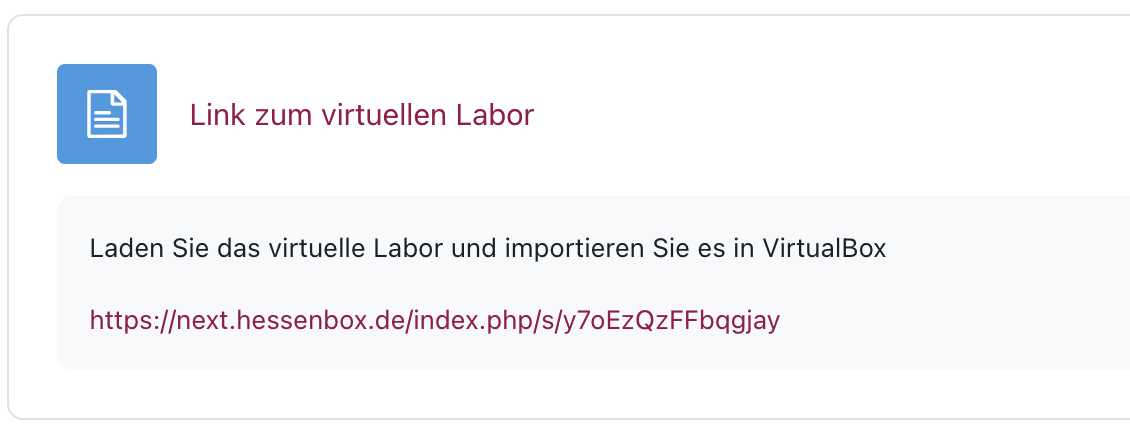
\includegraphics[width=0.7\textwidth]{images/img_Download-Link-IES-Labor-auf-moodle.png}

\subsection{Datei konvertieren}

\subsubsection{Installieren der benötigten Programme}

Für die Konvertierung benötigen Sie folgende Programme:

\begin{tcolorbox}[title=Terminal-Befehl,colback=gray!10,colframe=gray!50!black,fontupper=\small]
\begin{lstlisting}
brew install utm qemu
\end{lstlisting}
\end{tcolorbox}

\subsubsection{In .tgz umwandeln}

Folgen Sie diesen Schritten, um die heruntergeladene Datei umzuwandeln:

\begin{enumerate}[label=\arabic*.,leftmargin=1.5em,itemsep=0.3em]
  \item Öffnen Sie das Terminal
  \item Wechseln Sie zum Download-Verzeichnis:
    \begin{tcolorbox}[colback=gray!5,colframe=gray!40,boxrule=0.5pt,arc=0pt,left=2pt,right=2pt,top=1pt,bottom=1pt]
    \lstinline{cd Download}
    \end{tcolorbox}
  \item Benennen Sie die Datei um:
    \begin{tcolorbox}[colback=gray!5,colframe=gray!40,boxrule=0.5pt,arc=0pt,left=2pt,right=2pt,top=1pt,bottom=1pt]
    \lstinline{mv IES-Labor\ V0425.ova IES-Labor.tgz}
    \end{tcolorbox}
\end{enumerate}

\begin{figure}[H]
    \centering
    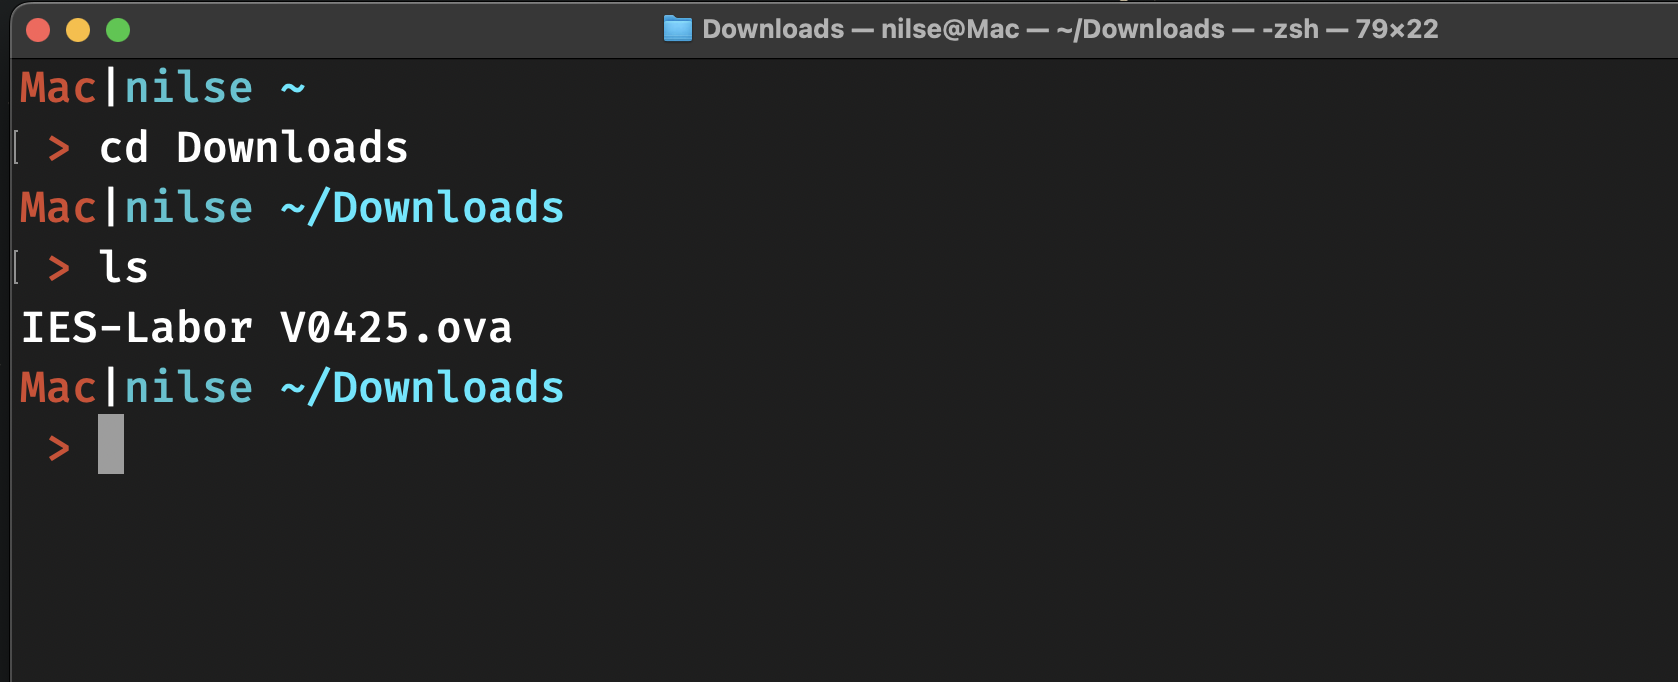
\includegraphics[width=0.48\textwidth]{images/img_cd-nach-download-und-ls.png}
    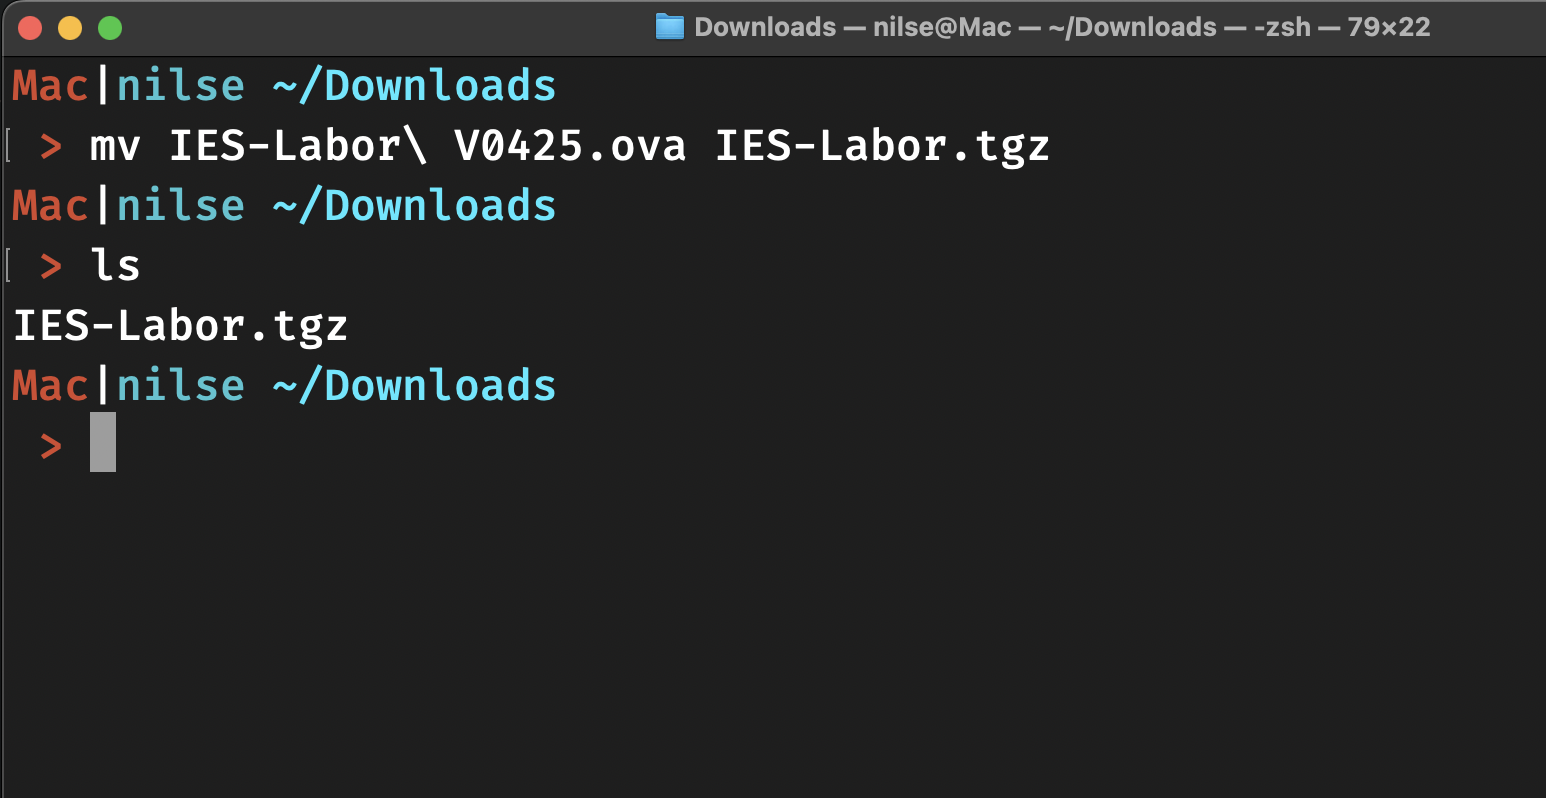
\includegraphics[width=0.48\textwidth]{images/img_rename-downloaded-file.png}
    \caption{Terminal-Befehle zum Wechseln des Verzeichnisses und Umbenennen der Datei}
    \label{fig:terminal-befehle}
\end{figure}

Die Durchführung der Schritte 1-3 ist in Abbildung \ref{fig:terminal-befehle} visualisiert.

\begin{tcolorbox}[title=Wichtig,colback=yellow!10,colframe=yellow!50!black]
Bitte beachten Sie, dass die Dateinamen (wie \datei{IES-Labor V0425.ova}) exakt mit den tatsächlichen Dateinamen übereinstimmen müssen. 
Automatische Vervollständigung der Namen ist mit der [TAB]-Taste möglich.
\end{tcolorbox}

\begin{tcolorbox}[title=Tipp,colback=blue!10,colframe=blue!50!black]
Der Befehl \lstinline{ls} listet alle Dateien im aktuellen Verzeichnis auf.

Mit Zusätzen kann der Befehl modifiziert werden:
\begin{itemize}[leftmargin=1.5em,itemsep=0.1em]
    \item \lstinline{ls -l} \hfill \# Listenformat mit Details
    \item \lstinline{ls -a} \hfill \# Alle Dateien (auch versteckte)
\end{itemize}
\end{tcolorbox}

\subsubsection{Entpacken und Konvertieren}

\begin{enumerate}[label=\arabic*.,leftmargin=1.5em,itemsep=0.3em]
  \item Entpacken Sie die Datei mit:
    \begin{tcolorbox}[colback=gray!5,colframe=gray!40,boxrule=0.5pt,arc=0pt,left=2pt,right=2pt,top=1pt,bottom=1pt]
    \lstinline{tar xvf IES-Labor.tgz}
    \end{tcolorbox}
    
  \item Konvertieren Sie die entpackte Datei für den QEMU-Hypervisor:
    \begin{tcolorbox}[colback=gray!5,colframe=gray!40,boxrule=0.5pt,arc=0pt,left=2pt,right=2pt,top=1pt,bottom=1pt]
    \lstinline{qemu-img convert -O qcow2 IES-Labor\ V0425-disk001.vmdk IES-Labor.qcow2}
    \end{tcolorbox}
\end{enumerate}

\begin{figure}[H]
    \centering
    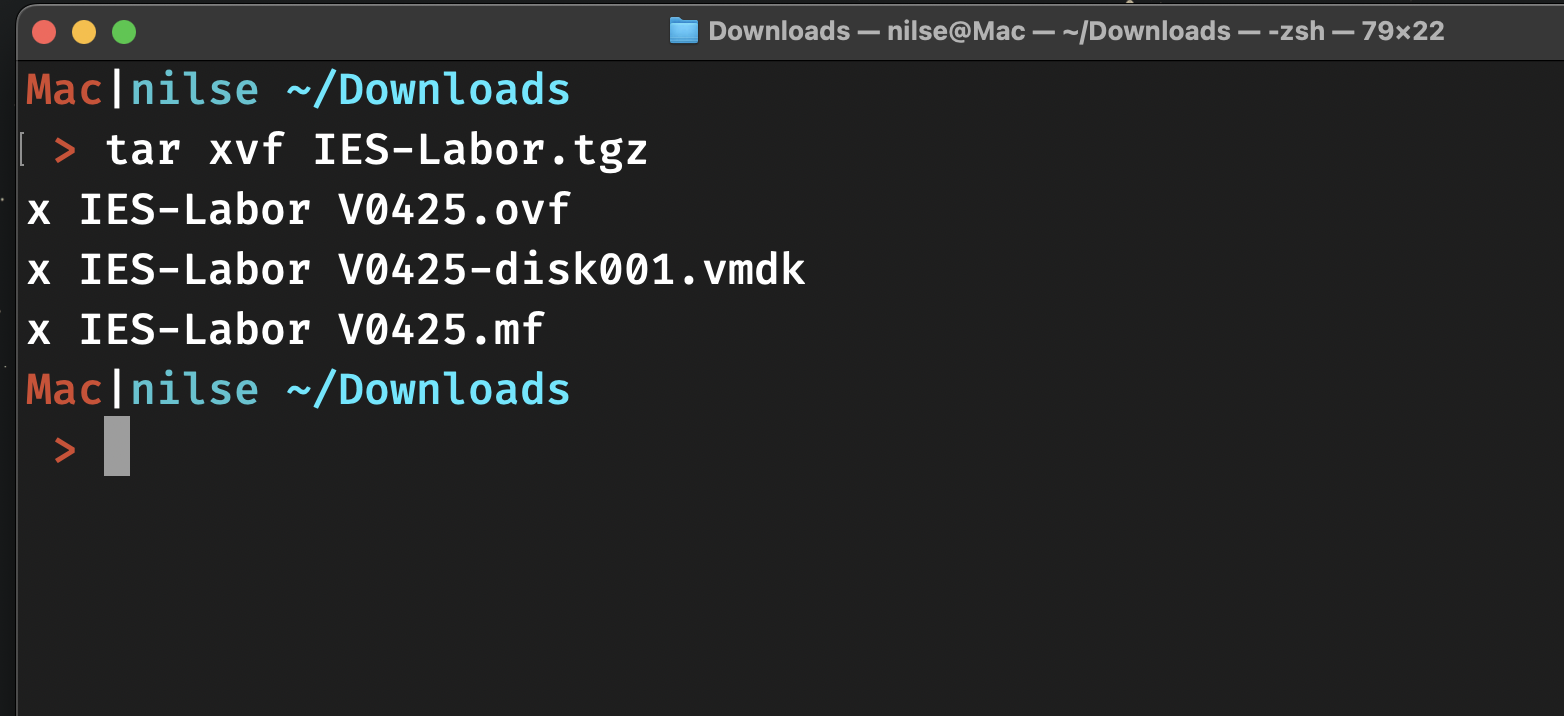
\includegraphics[width=0.48\textwidth]{images/img_tgz-entpacken.png}
    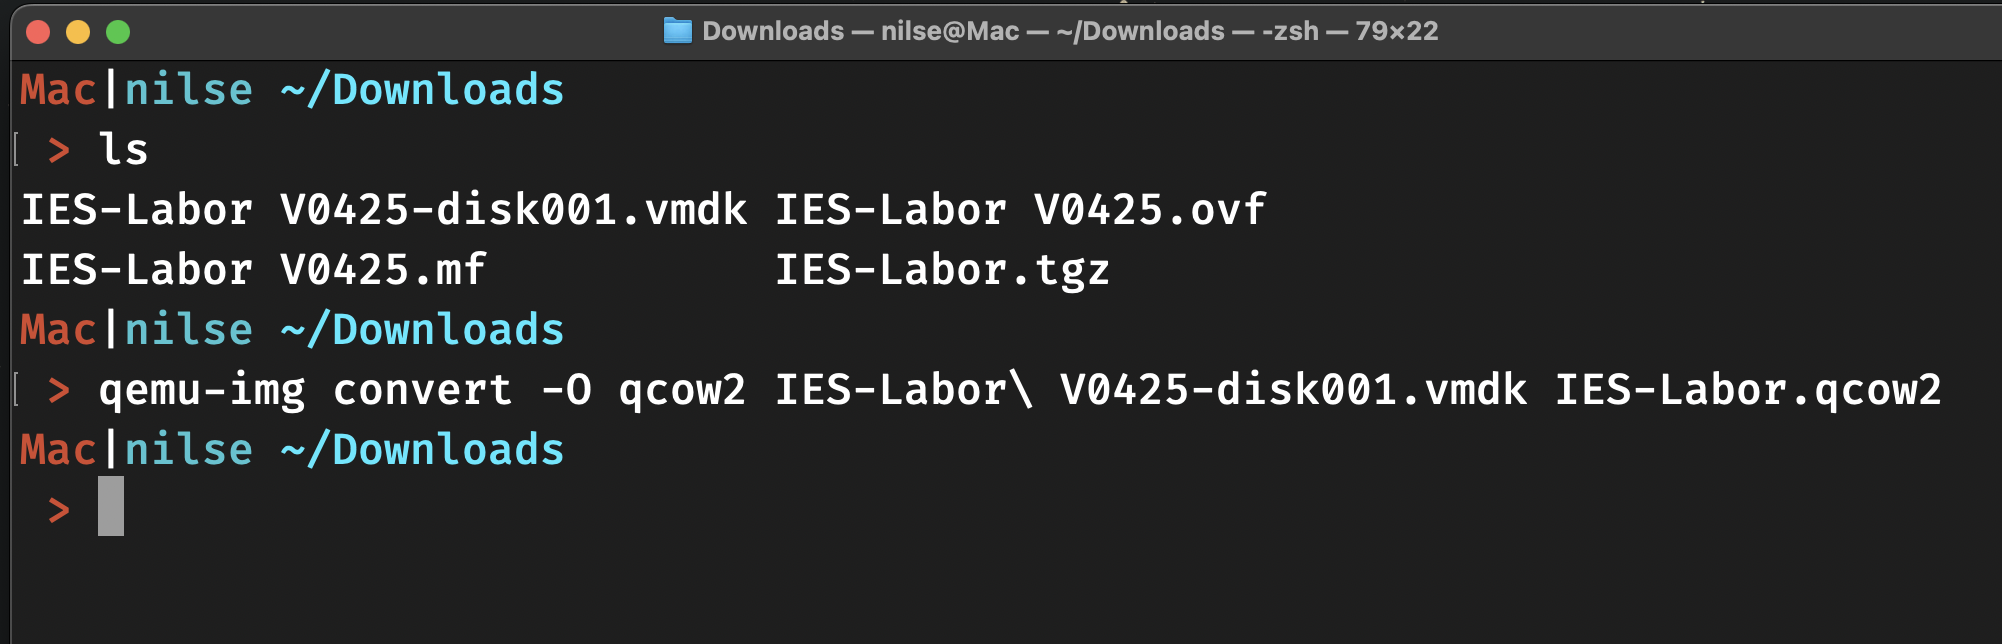
\includegraphics[width=0.48\textwidth]{images/img_ls-und-datei-convertieren-mit-qemu.png}
    \caption{Entpacken der TGZ-Datei und Konvertierung in das QCOW2-Format}
    \label{fig:entpacken-konvertieren}
\end{figure}

Die Durchführung der Schritte 1-2 ist in Abbildung \ref{fig:entpacken-konvertieren} dargestellt.

\subsection{VM erstellen}

\subsubsection{Öffnen von UTM}\label{sec:Öffnen von UTM} % (fold)

UTM hat bei mir nicht funktioniert nach dem Installieren, das Programm ist immer gecrashed und hat nur einen Crash-Report von Apple angezeigt. Auch der Neustart des Rechners hat nicht geholfen.

Meine einzige gefundene Lösung ist das Updaten auf die neuste Version von MacOS. Ich habe die beta-version Sequoia 15.5 Beta (24F5068ba) installiert, worauf UTM funktioniert.

% subsubsection Öffnen von UTM (end)

\subsubsection{Neue VM in UTM erstellen}

\begin{enumerate}[label=\arabic*.,leftmargin=1.5em,itemsep=0.3em]
  \item Erstellen Sie eine neue virtuelle Maschine
  \item Wählen Sie als Typ: \textbf{Emulate}
\end{enumerate}

\begin{figure}[H]
    \centering
    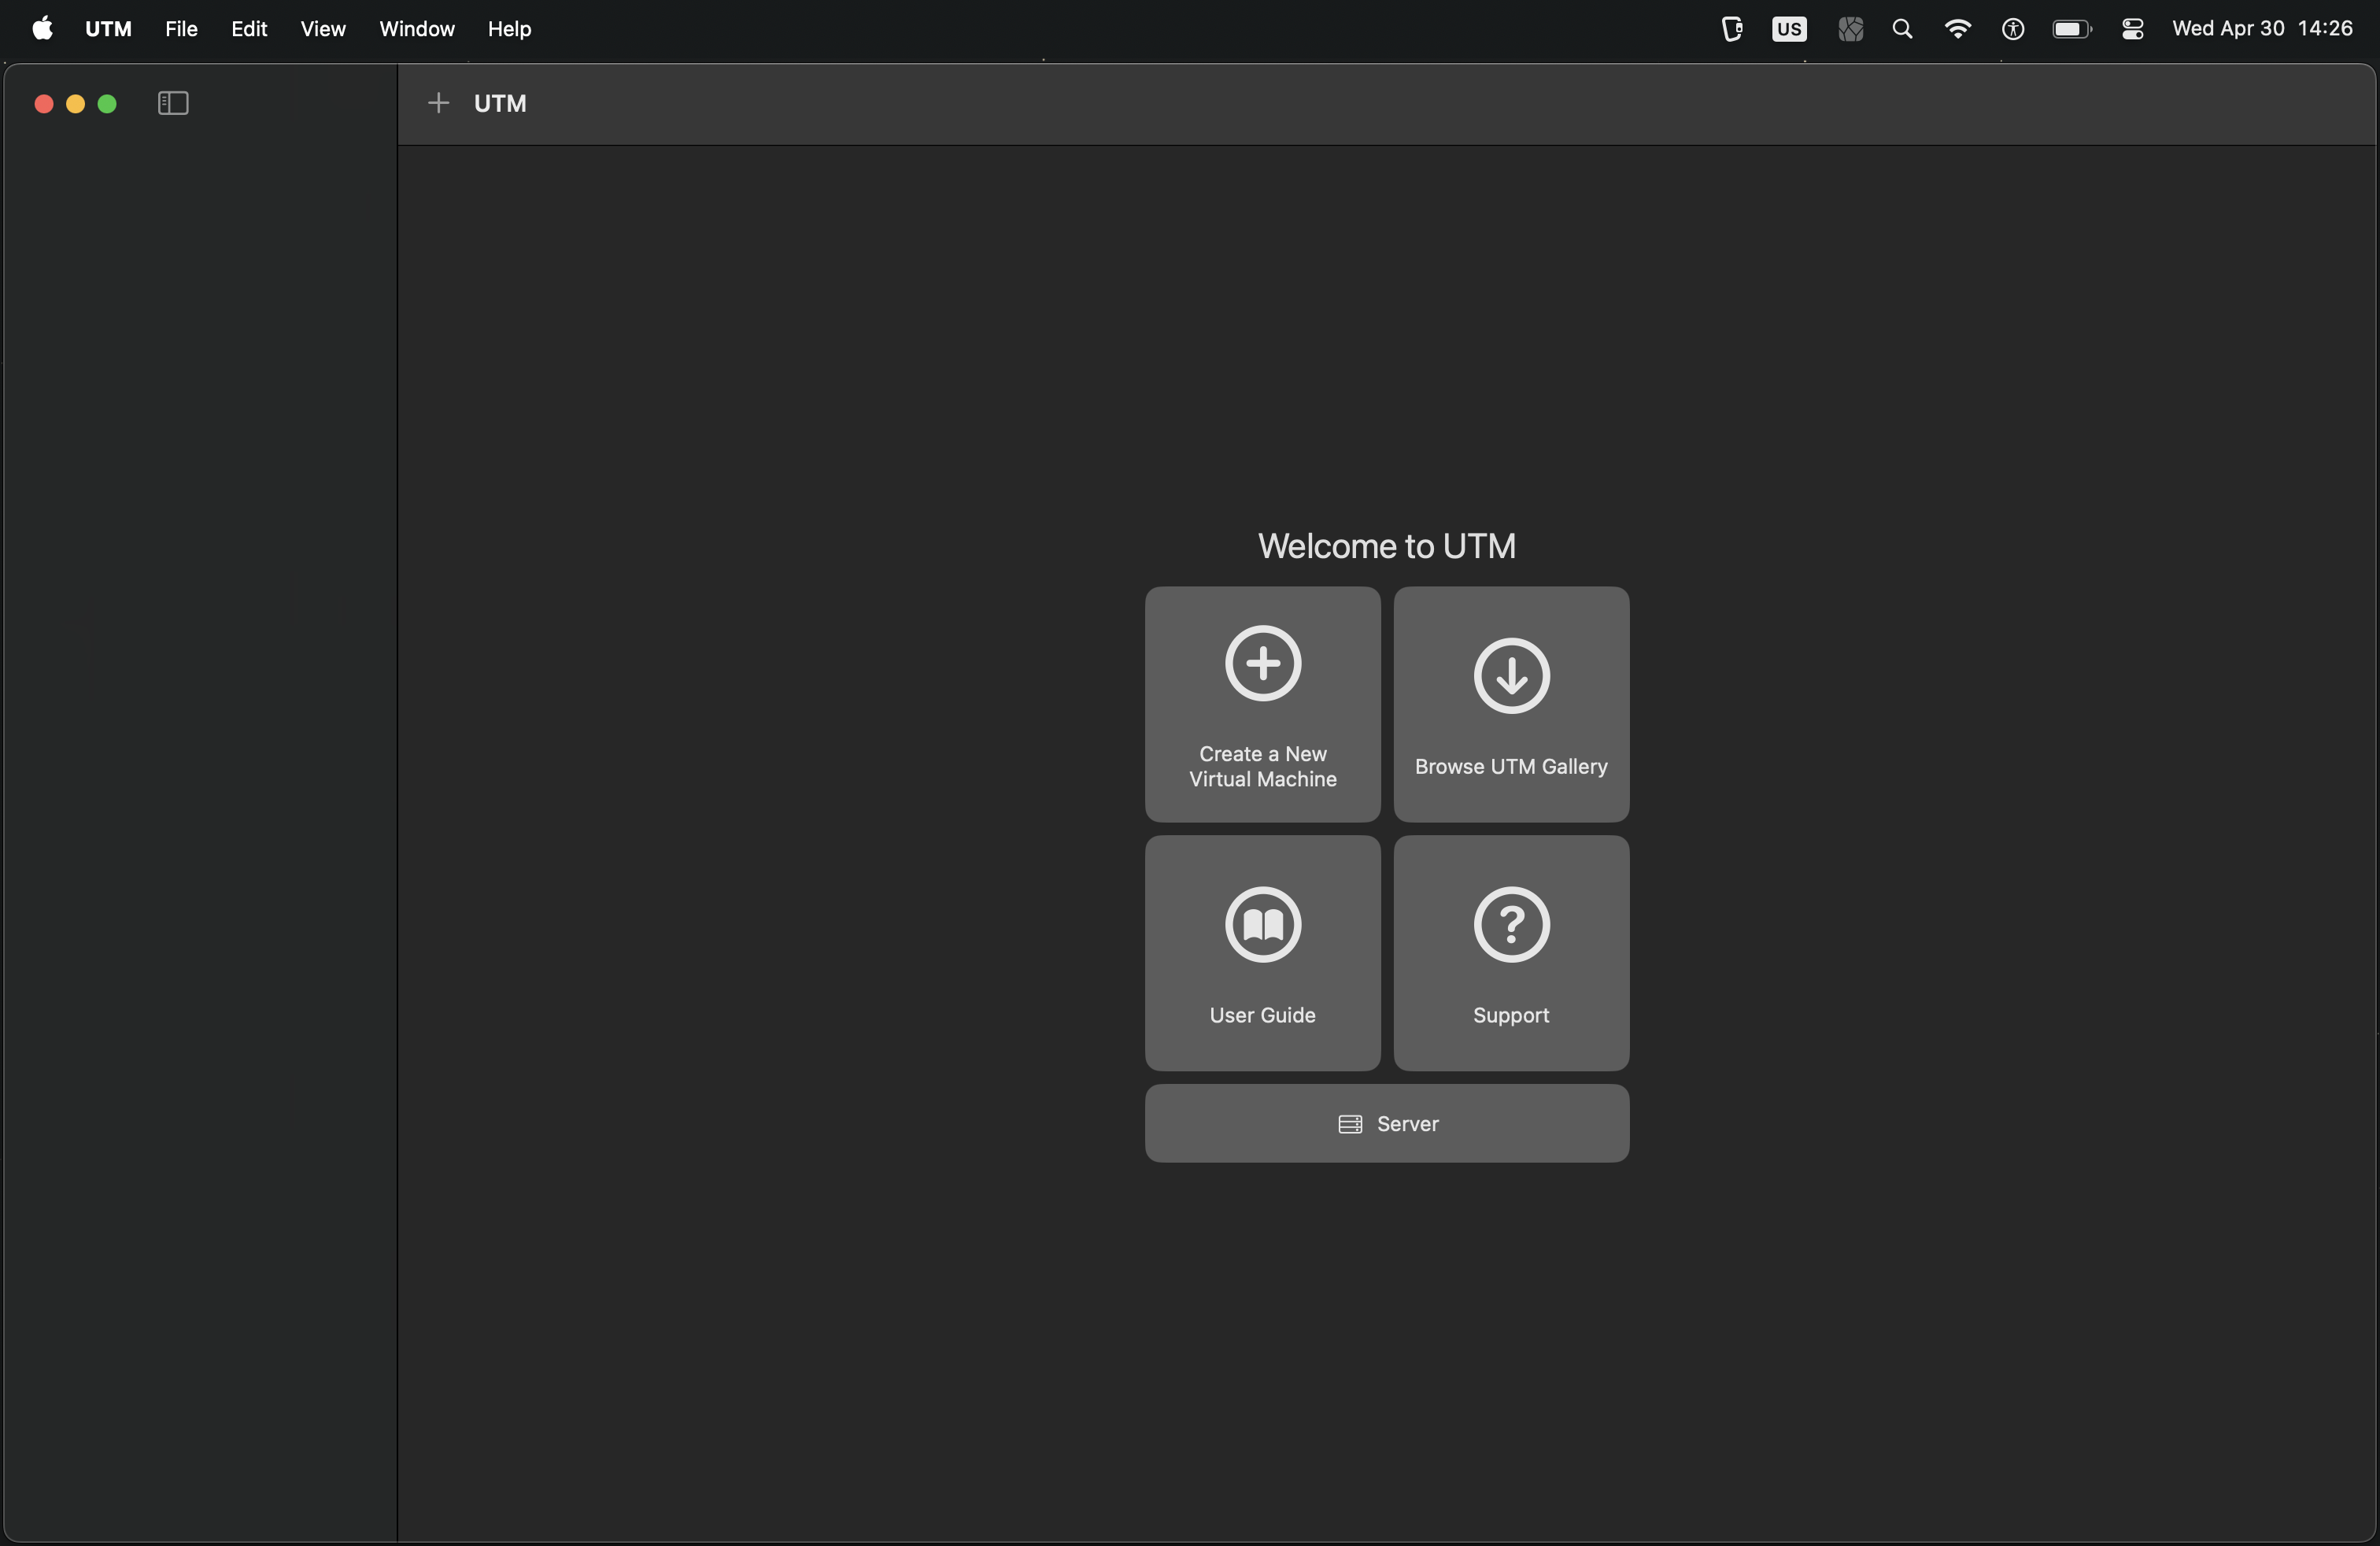
\includegraphics[width=0.48\textwidth]{images/img_utm_create-new-vm.png}
    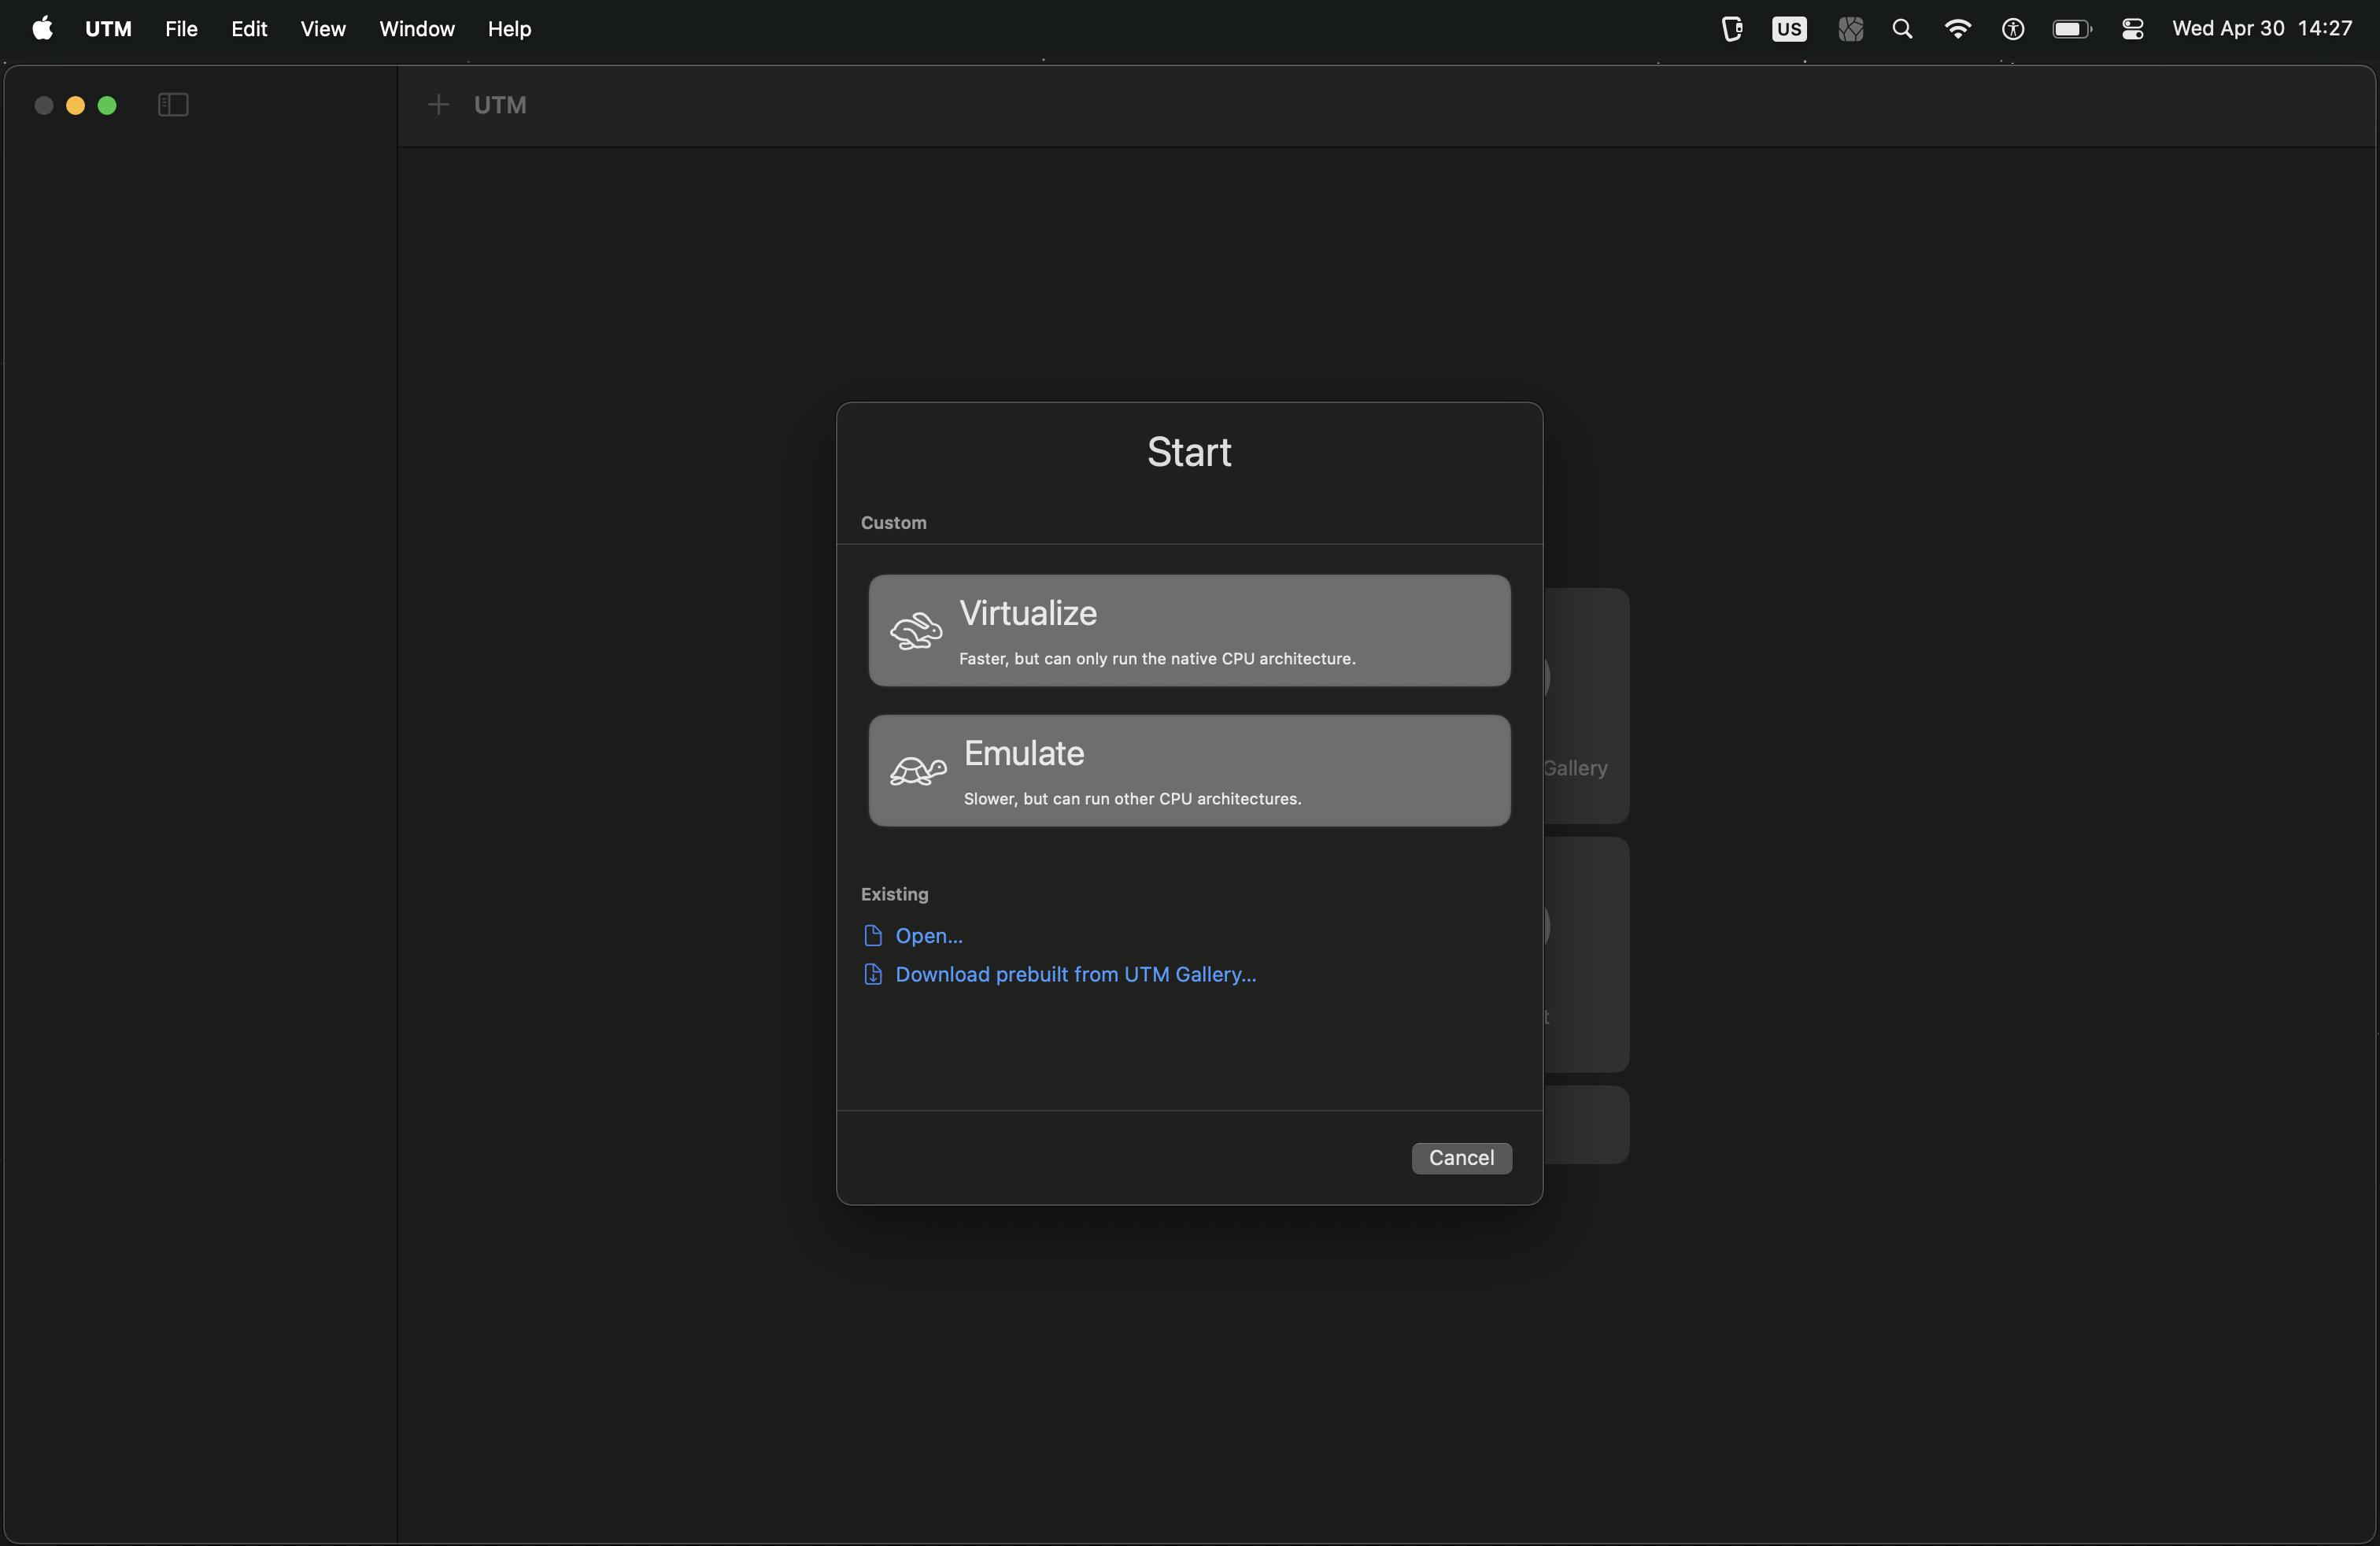
\includegraphics[width=0.48\textwidth]{images/img_utm_emulation.png}
    \caption{Neue VM erstellen und Emulation auswählen}
    \label{fig:vm-erstellen-emulation}
\end{figure}

Die Umsetzung der Schritte 1-2 ist in Abbildung \ref{fig:vm-erstellen-emulation} zu sehen.

\begin{enumerate}[label=\arabic*.,leftmargin=1.5em,itemsep=0.3em,start=3]
  \item Wählen Sie als Betriebssystem: \textbf{Other}
  \item Wählen Sie als Boot Device: \textbf{None}
\end{enumerate}

\begin{figure}[H]
    \centering
    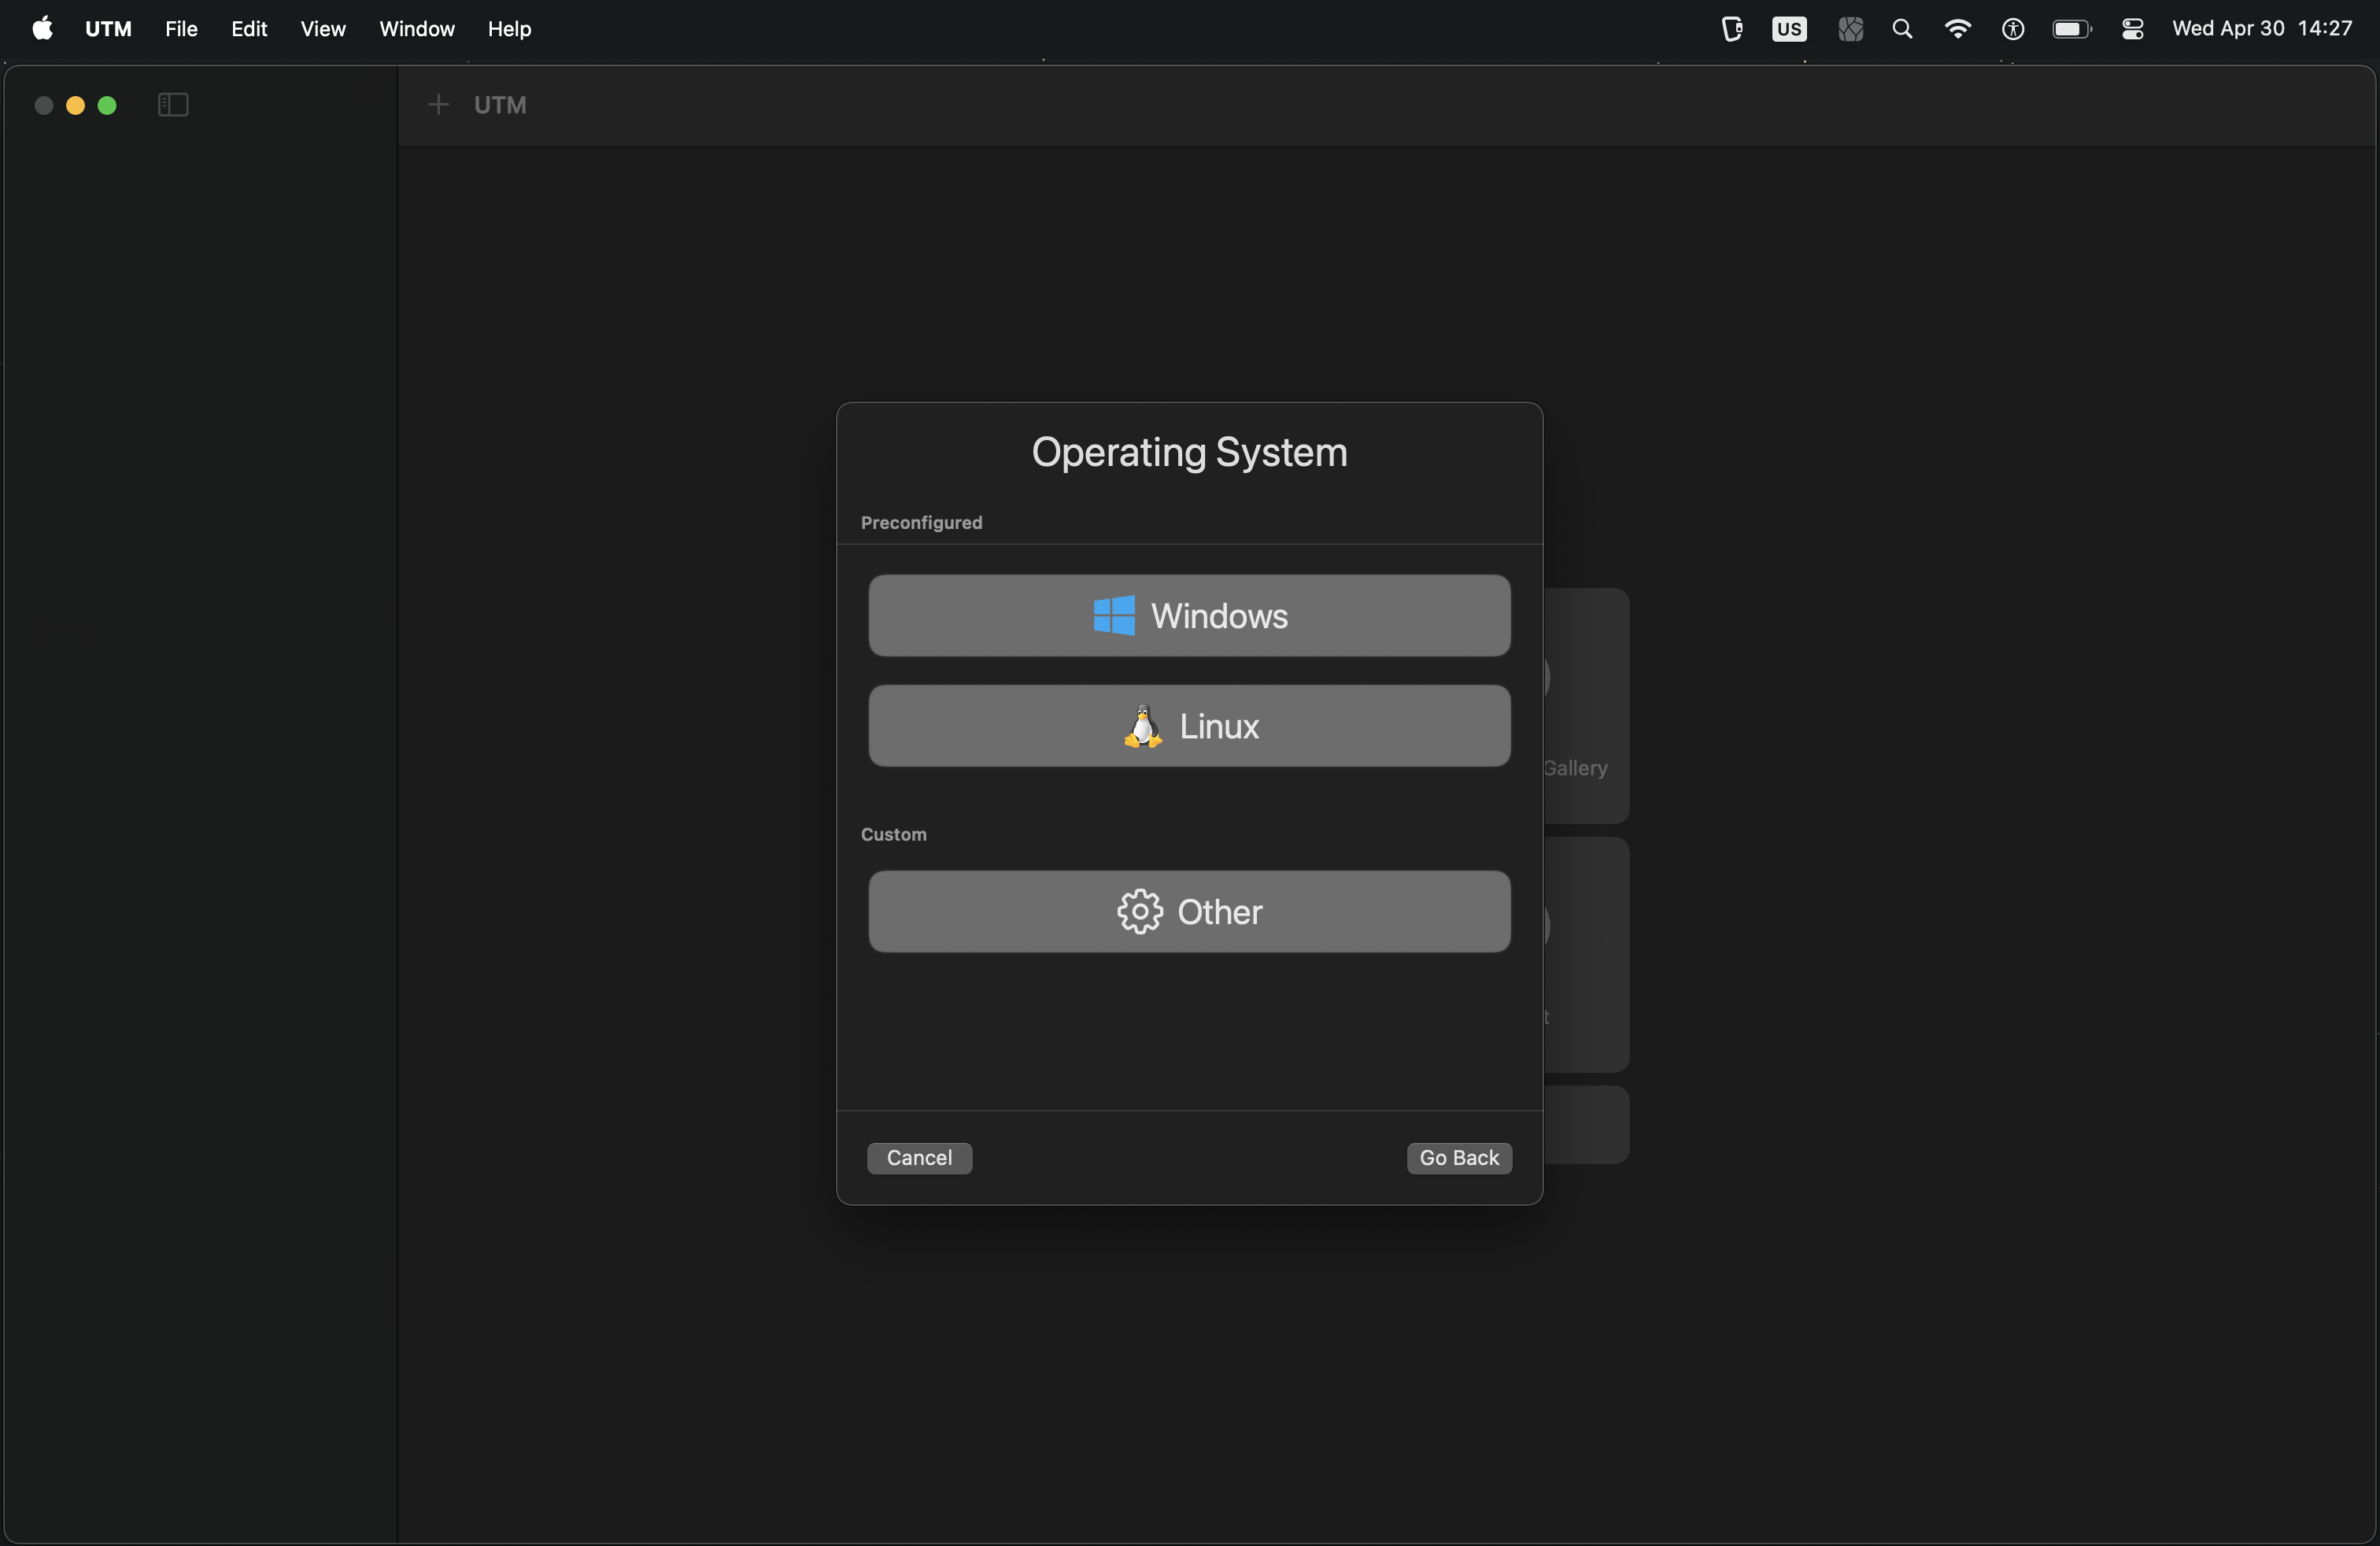
\includegraphics[width=0.48\textwidth]{images/img_utm_other.png}
    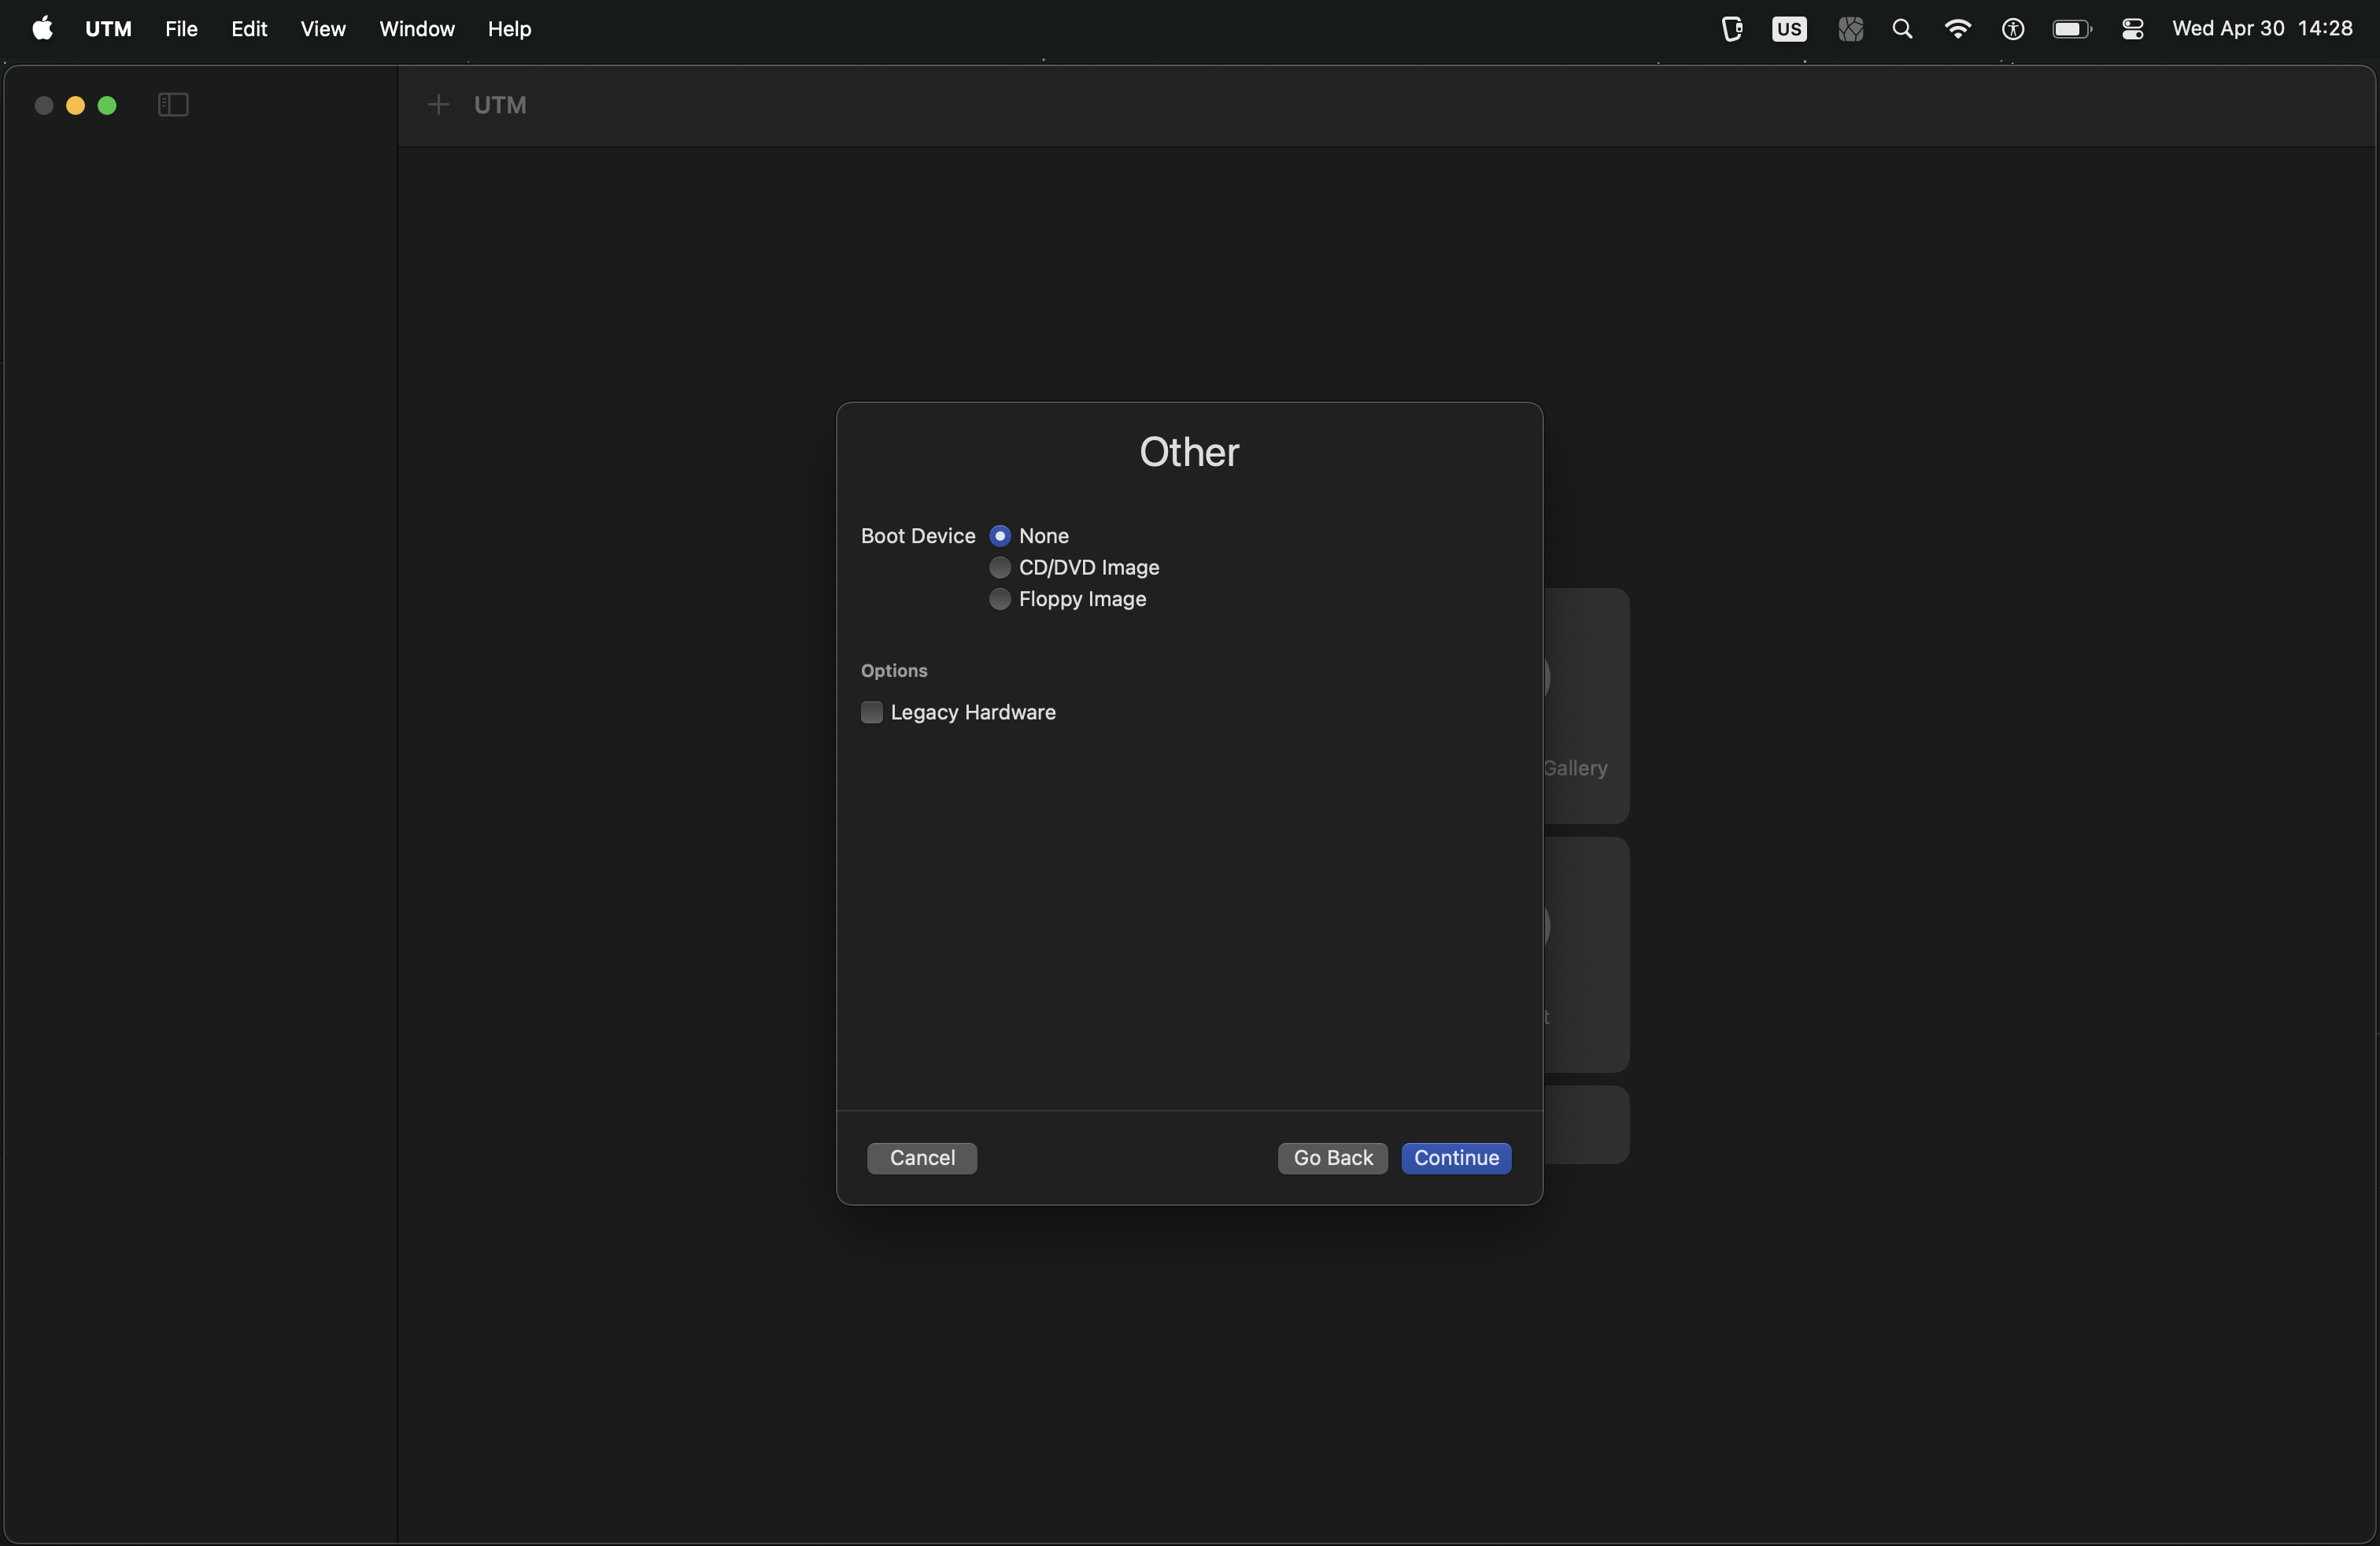
\includegraphics[width=0.48\textwidth]{images/img_utm_no-boot-device.png}
    \caption{Betriebssystem und Boot-Gerät auswählen}
    \label{fig:os-boot-device}
\end{figure}

Die Auswahl gemäß Schritt 3-4 ist in Abbildung \ref{fig:os-boot-device} dargestellt.

\begin{enumerate}[label=\arabic*.,leftmargin=1.5em,itemsep=0.3em,start=5]
  \item Konfigurieren Sie die Hardware-Einstellungen:
  \begin{itemize}[leftmargin=1.5em]
    \item Mindestens 1024 MB Arbeitsspeicher
    \item Mindestens 2 CPU-Kerne (Standardeinstellungen sind ausreichend)
  \end{itemize}
\end{enumerate}

\begin{figure}[H]
    \centering
    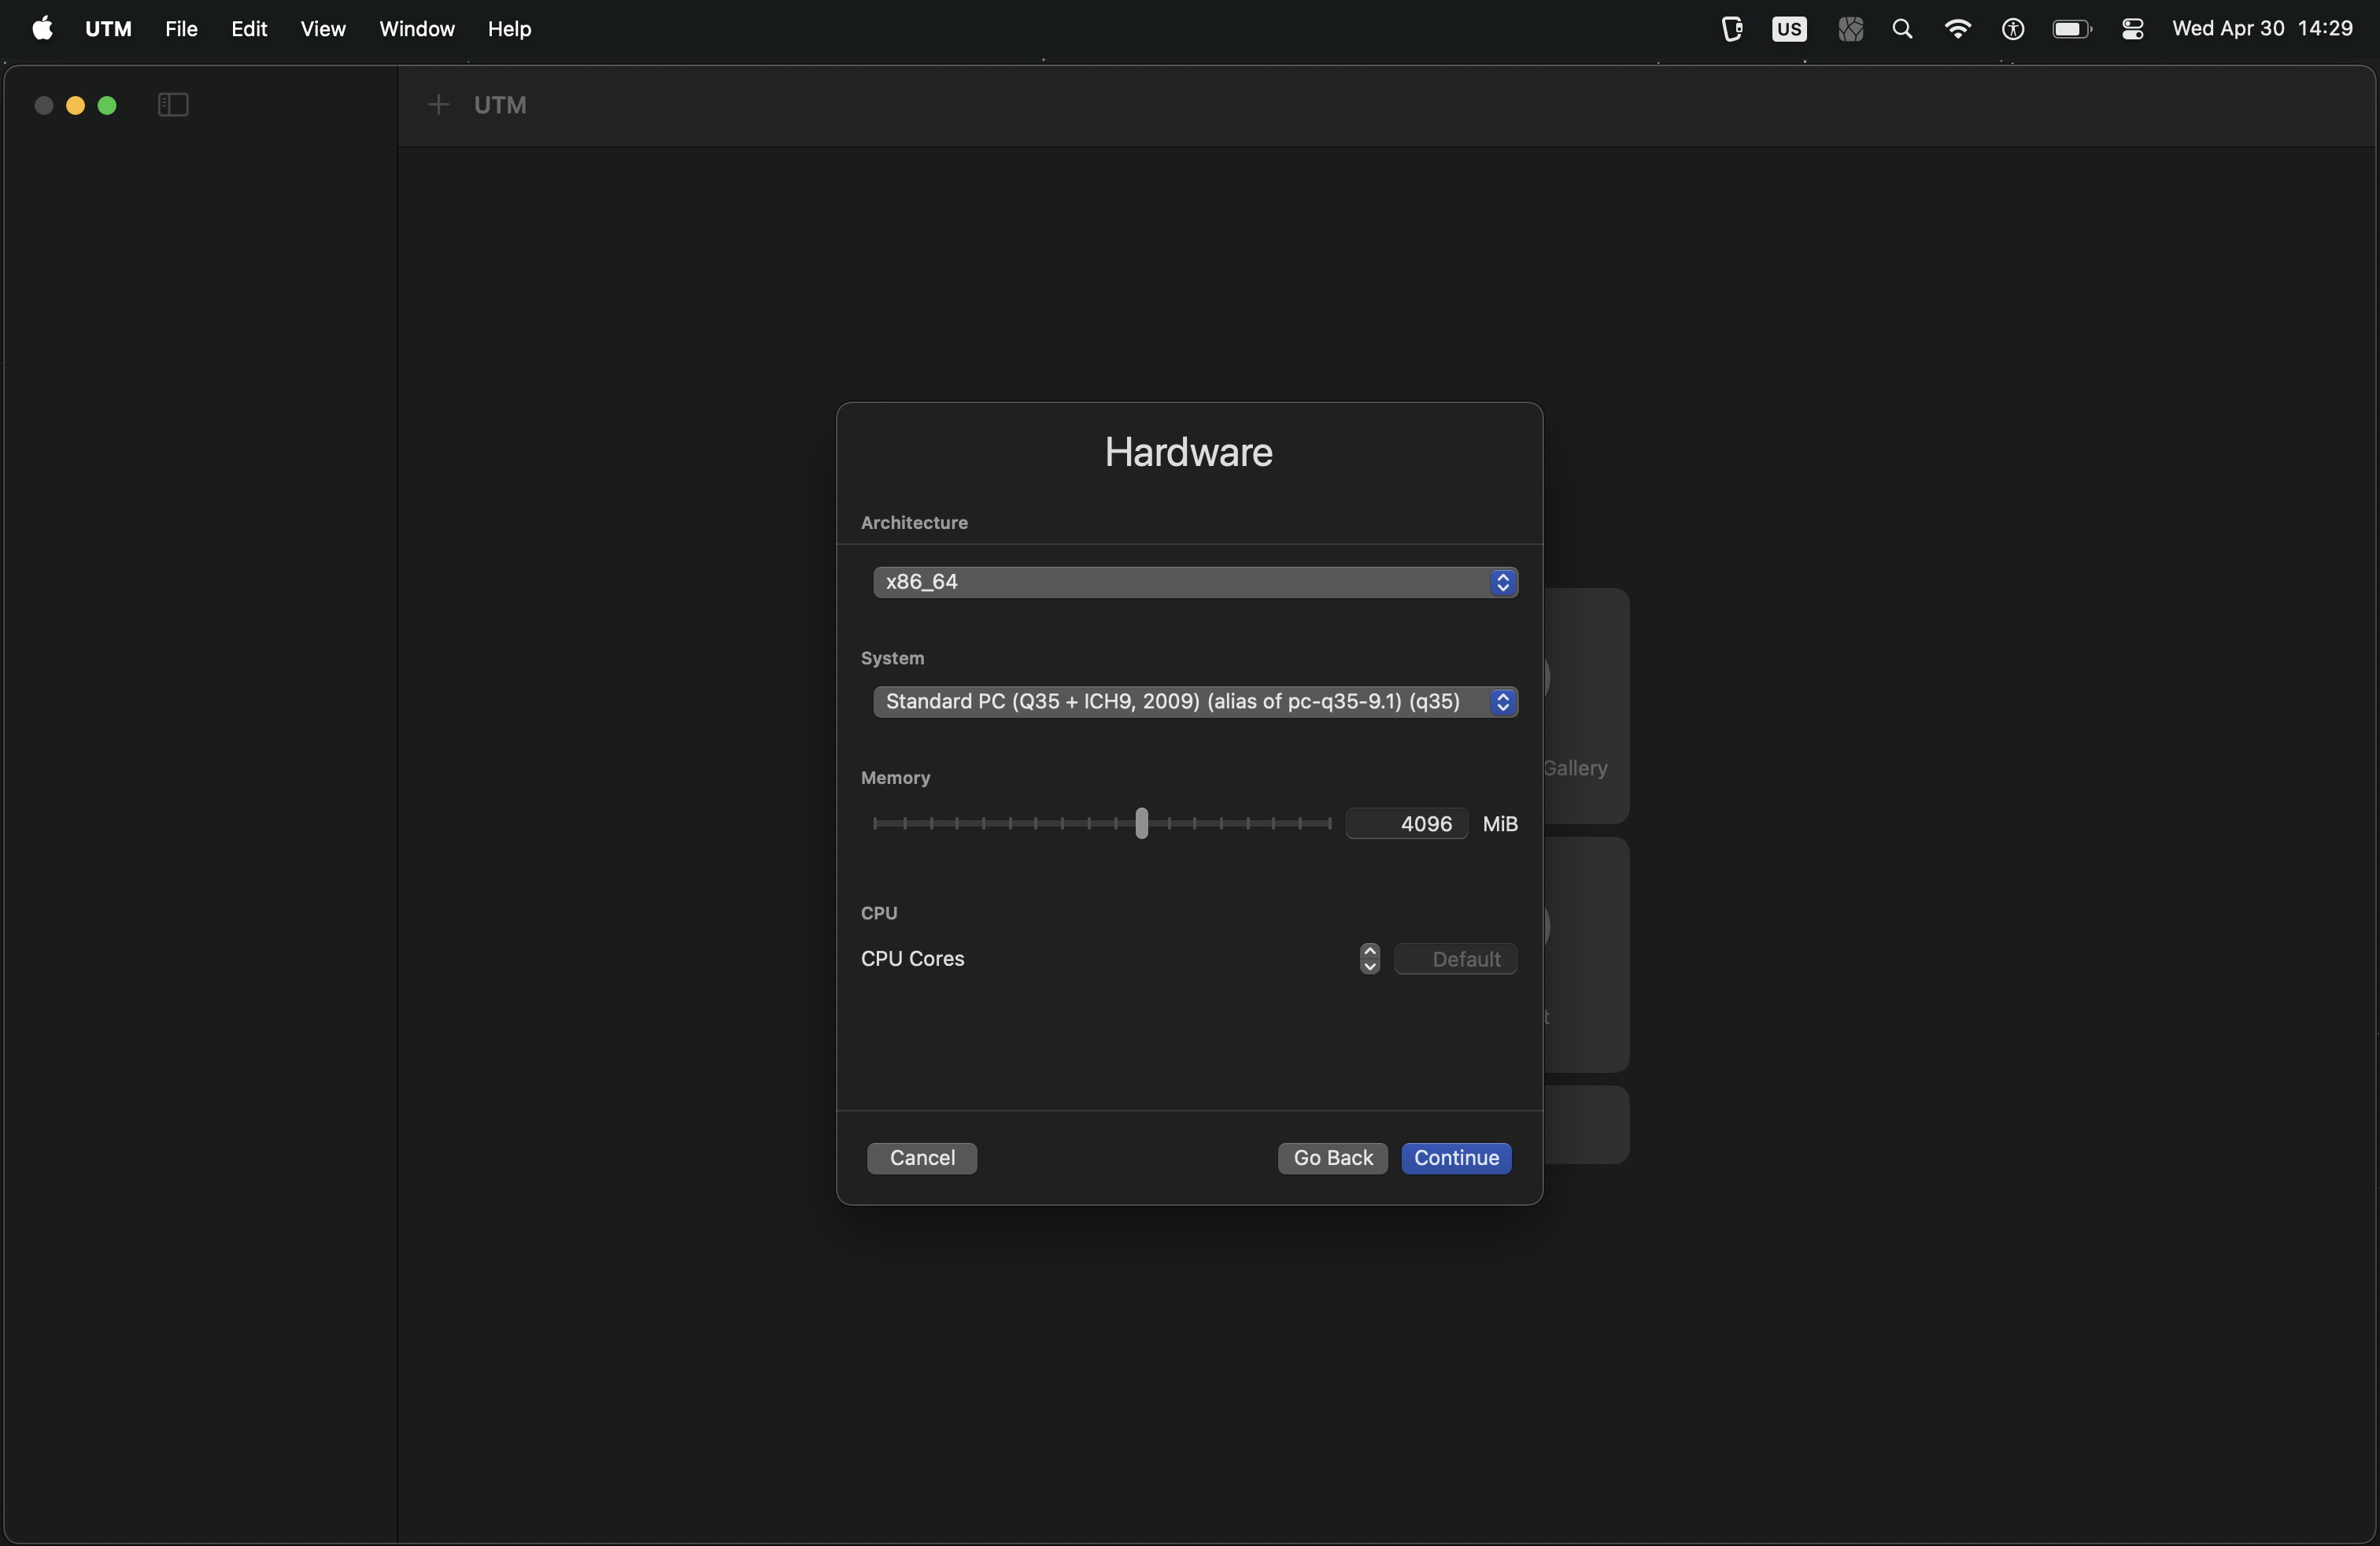
\includegraphics[width=0.7\textwidth]{images/img_utm_hardware-settings.png}
    \caption{Hardware-Einstellungen der VM}
    \label{fig:hardware-settings}
\end{figure}

Die Hardware-Konfiguration gemäß Schritt 5 ist in Abbildung \ref{fig:hardware-settings} zu sehen.

\begin{enumerate}[label=\arabic*.,leftmargin=1.5em,itemsep=0.3em,start=6]
  \item Legen Sie die Speichergröße fest
  \item Lassen Sie Shared Storage frei
  \item Beenden Sie das Setup
\end{enumerate}

\begin{figure}[H]
    \centering
    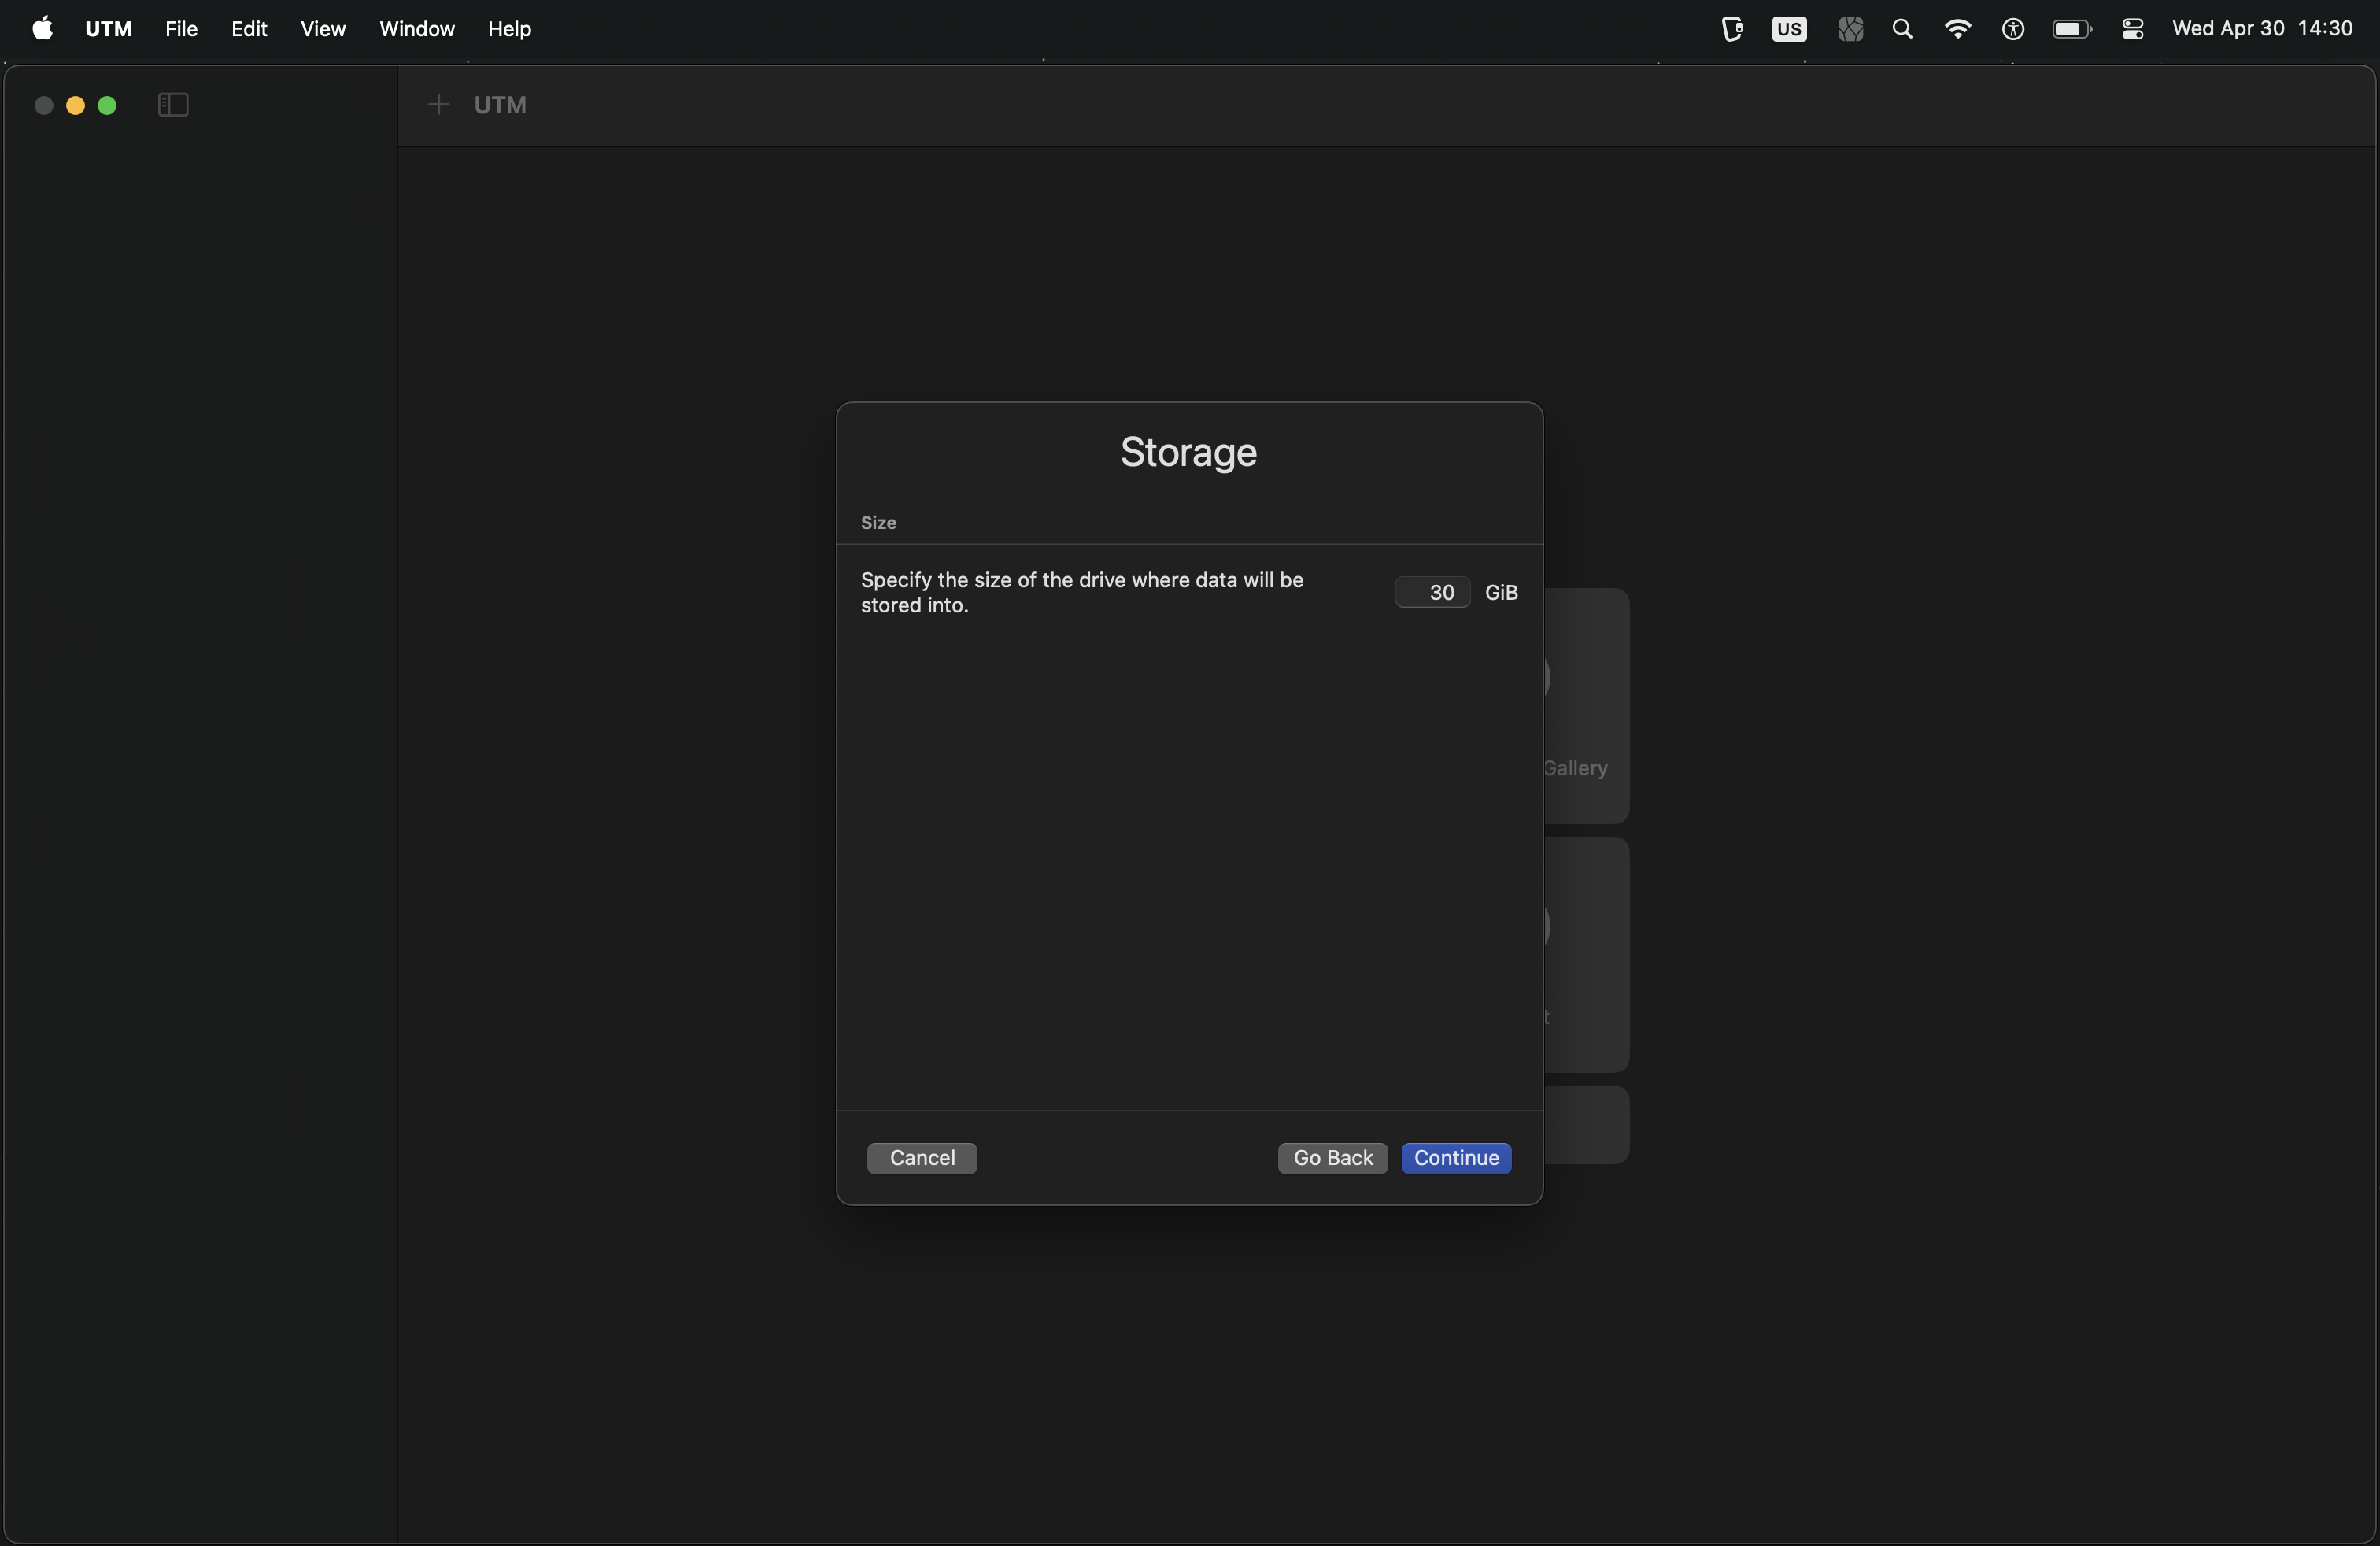
\includegraphics[width=0.48\textwidth]{images/img_utm_storage.png}
    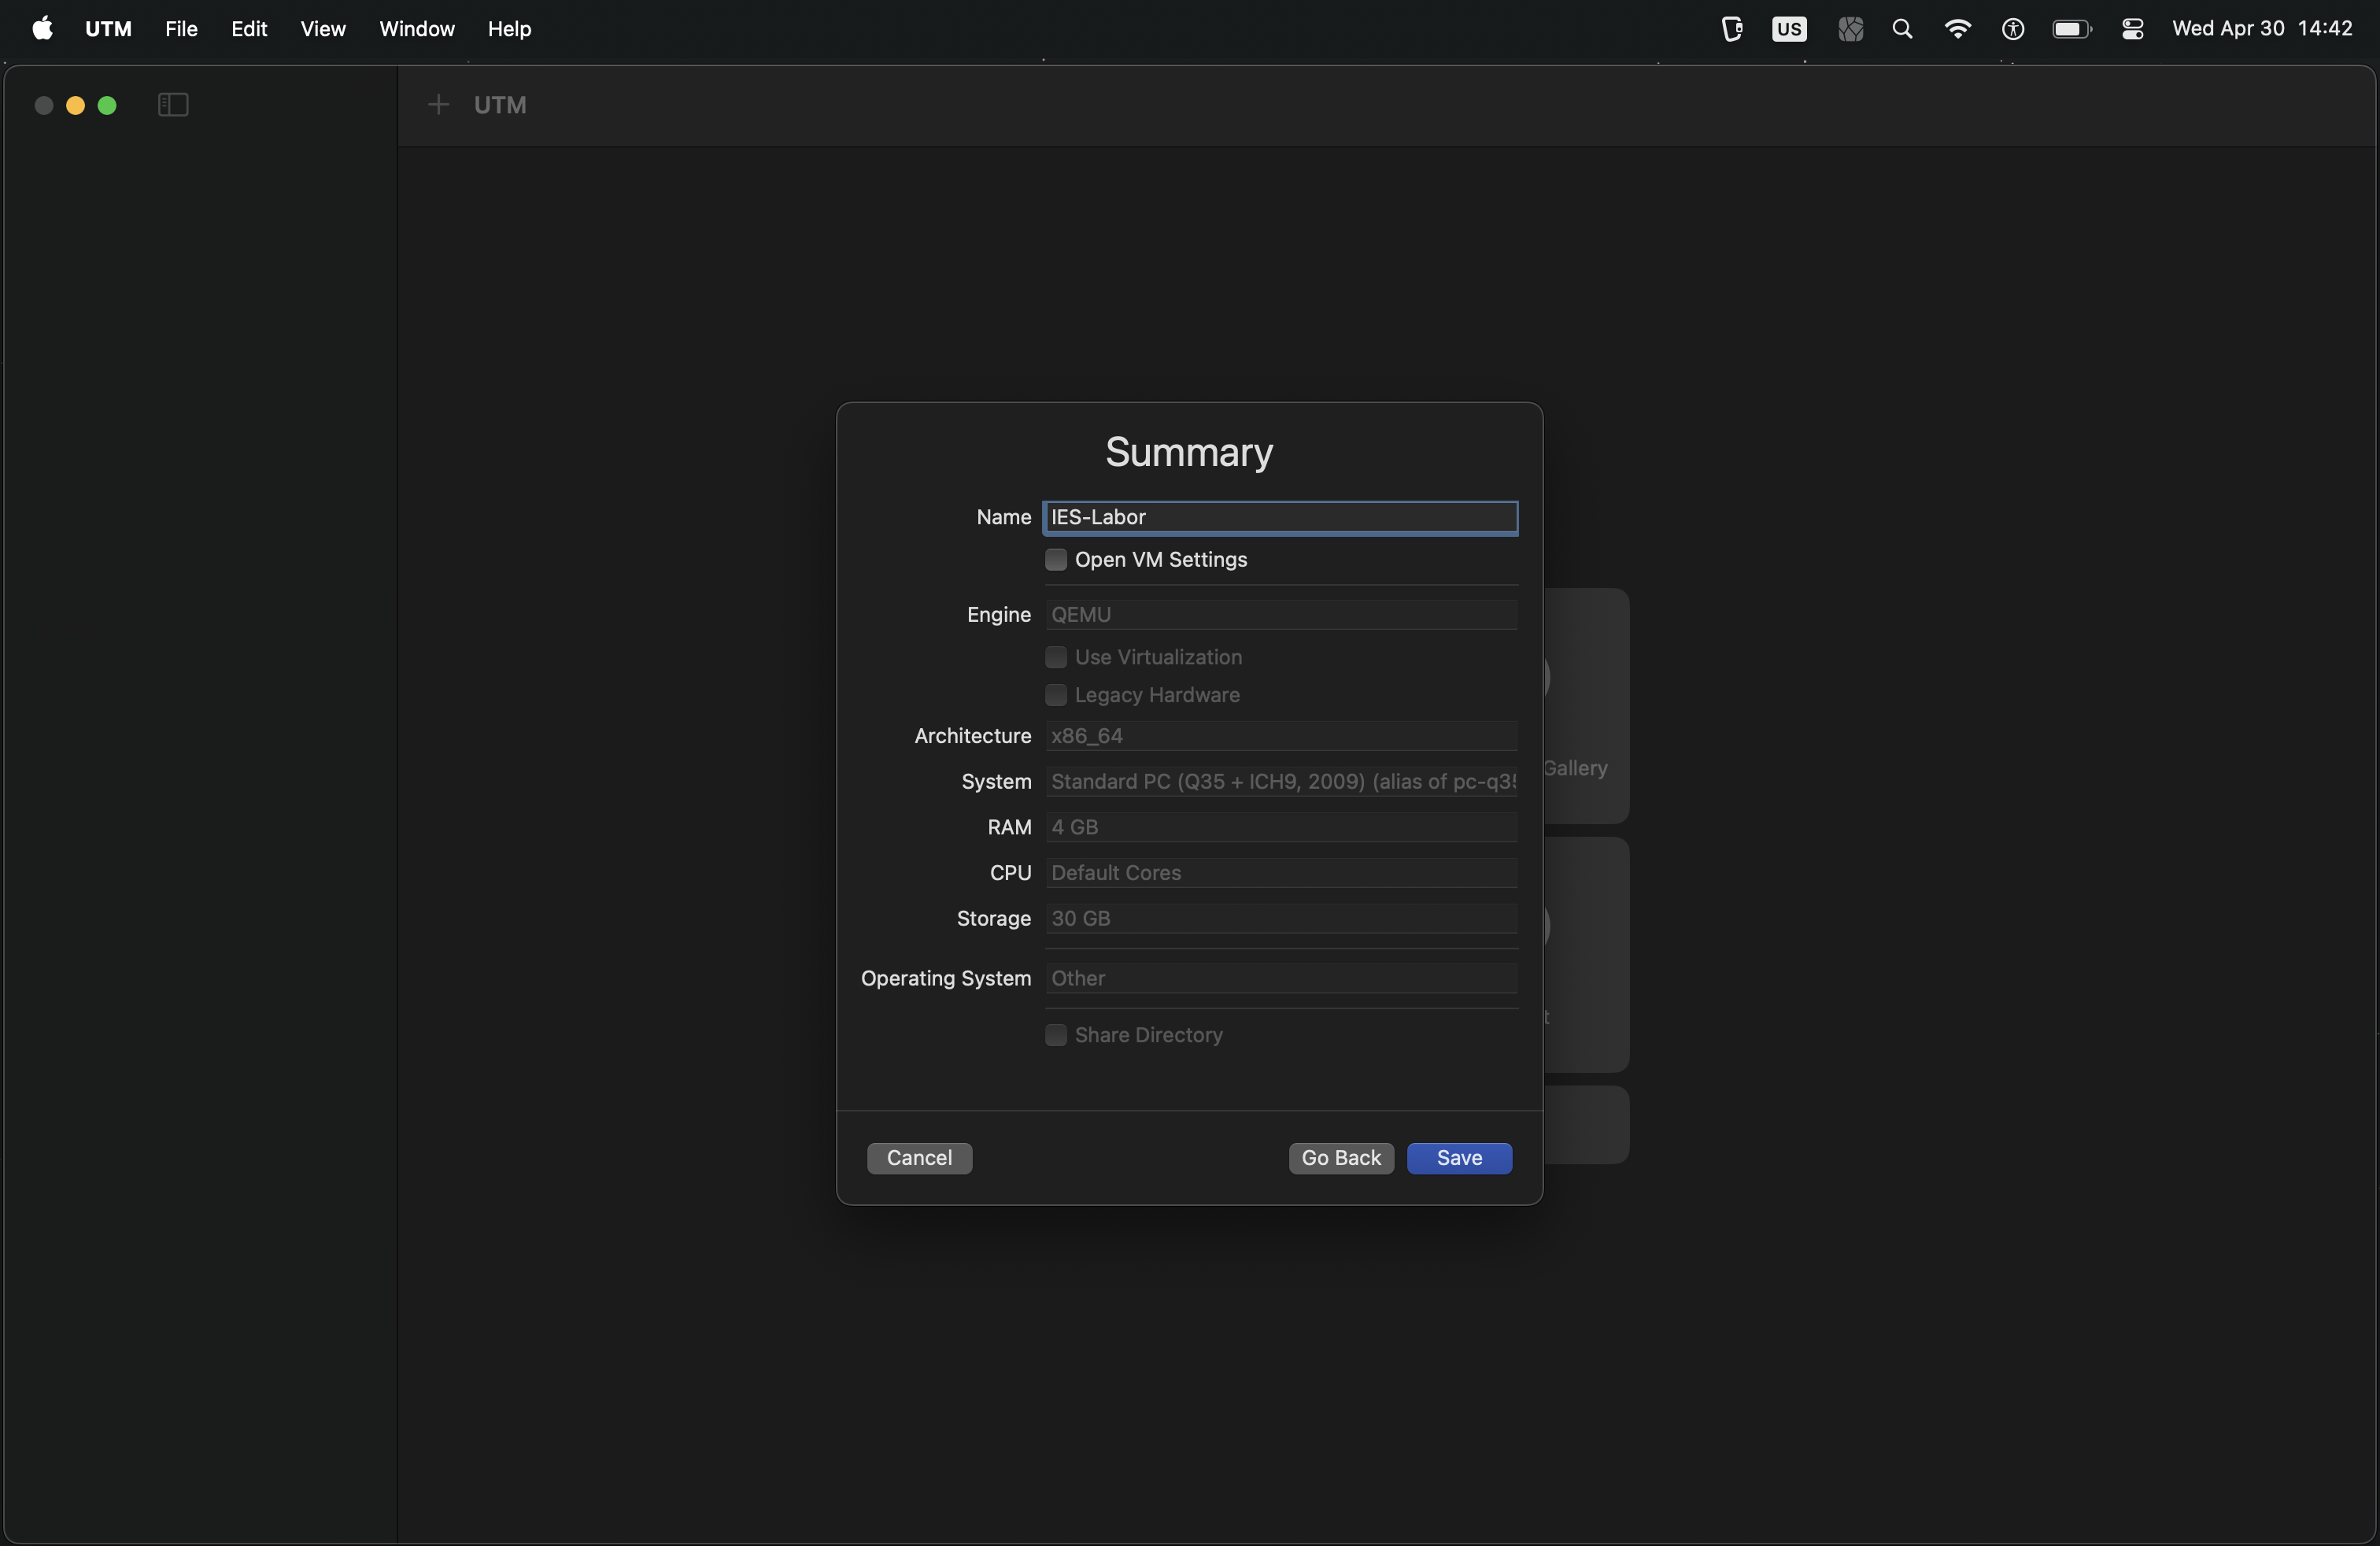
\includegraphics[width=0.48\textwidth]{images/img_utm_summary-benennung.png}
    \caption{Speichereinstellungen und Zusammenfassung}
    \label{fig:storage-summary}
\end{figure}

Die Einstellungen aus den Schritten 6-8 sind in Abbildung \ref{fig:storage-summary} dargestellt.

\subsection{VM-Einstellungen anpassen}

\begin{enumerate}[label=\arabic*.,leftmargin=1.5em,itemsep=0.3em]
  \item Bearbeiten Sie die VM über den \emph{Edit}-Button
\end{enumerate}

\begin{figure}[H]
    \centering
    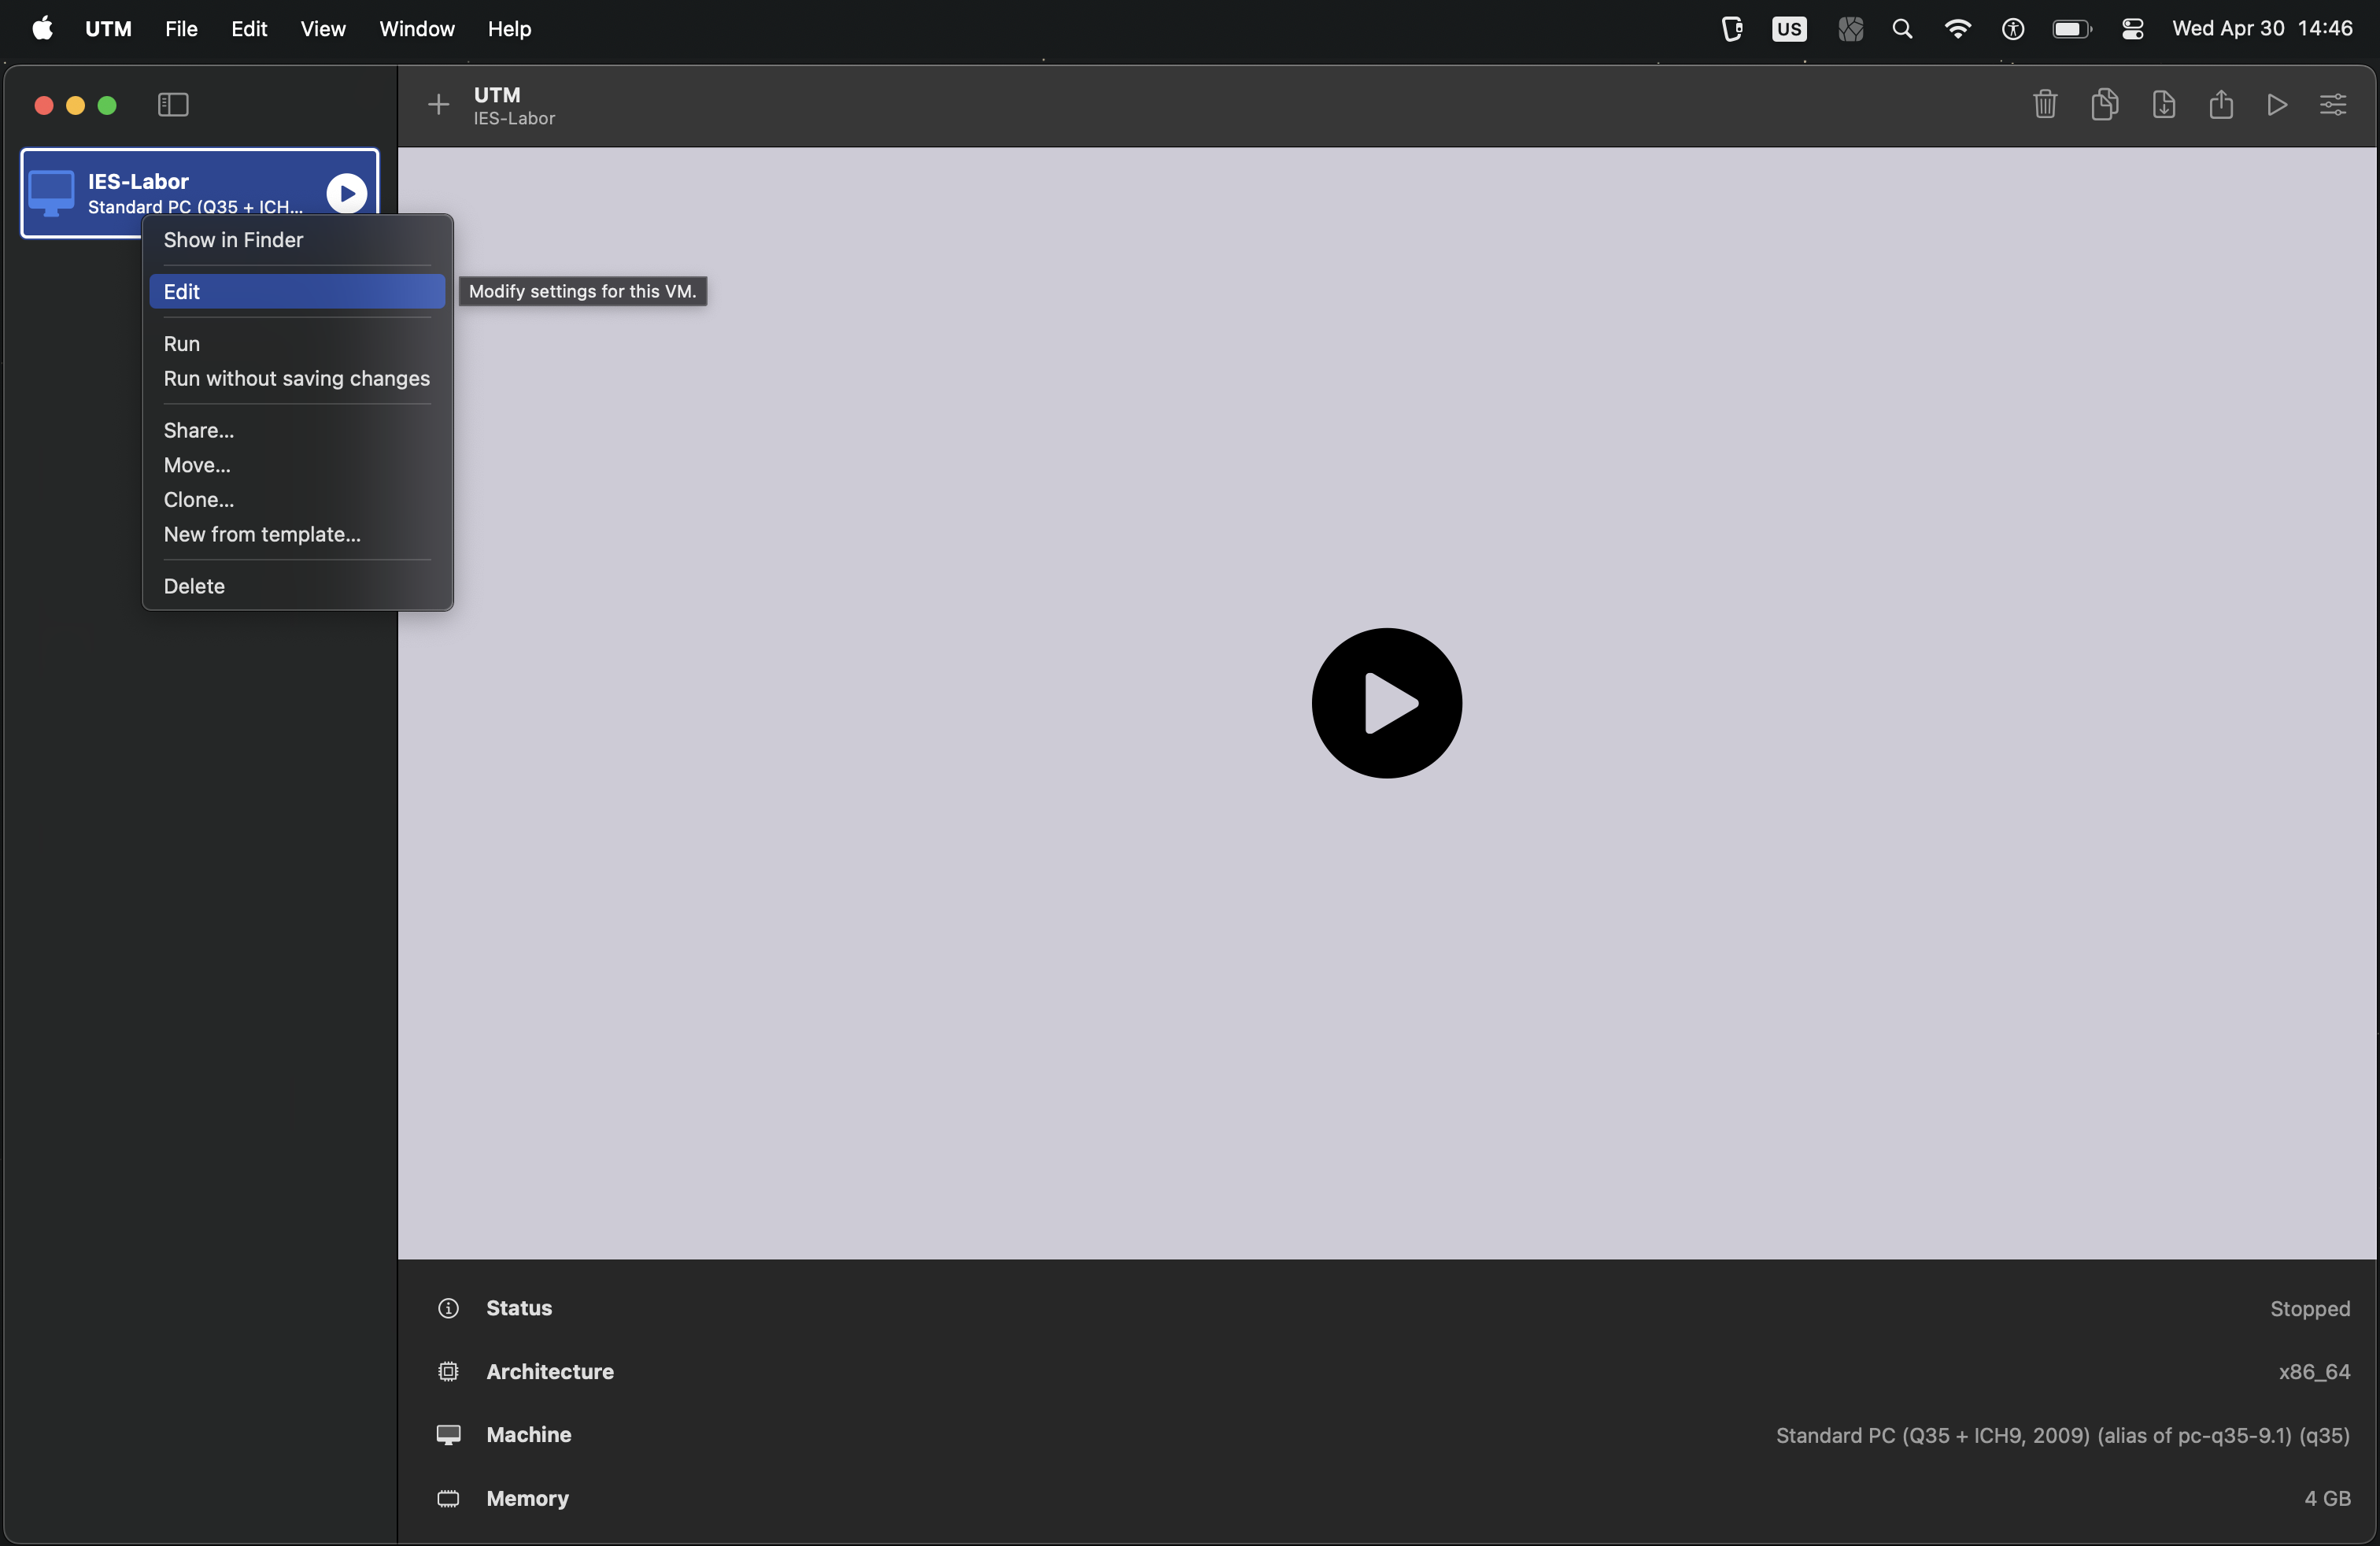
\includegraphics[width=0.7\textwidth]{images/img_utm_edit-vm.png}
    \caption{VM bearbeiten}
    \label{fig:edit-vm}
\end{figure}

Wie in Abbildung \ref{fig:edit-vm} zu sehen, können Sie die VM über den Edit-Button bearbeiten.

\begin{enumerate}[label=\arabic*.,leftmargin=1.5em,itemsep=0.3em,start=2]
	\item Aktivieren Sie unter System die Option \emph{Force Multicore}
  \item Deaktivieren Sie unter QEMU die Option \emph{UEFI-Boot}
\end{enumerate}

\begin{figure}[H]
    \centering
    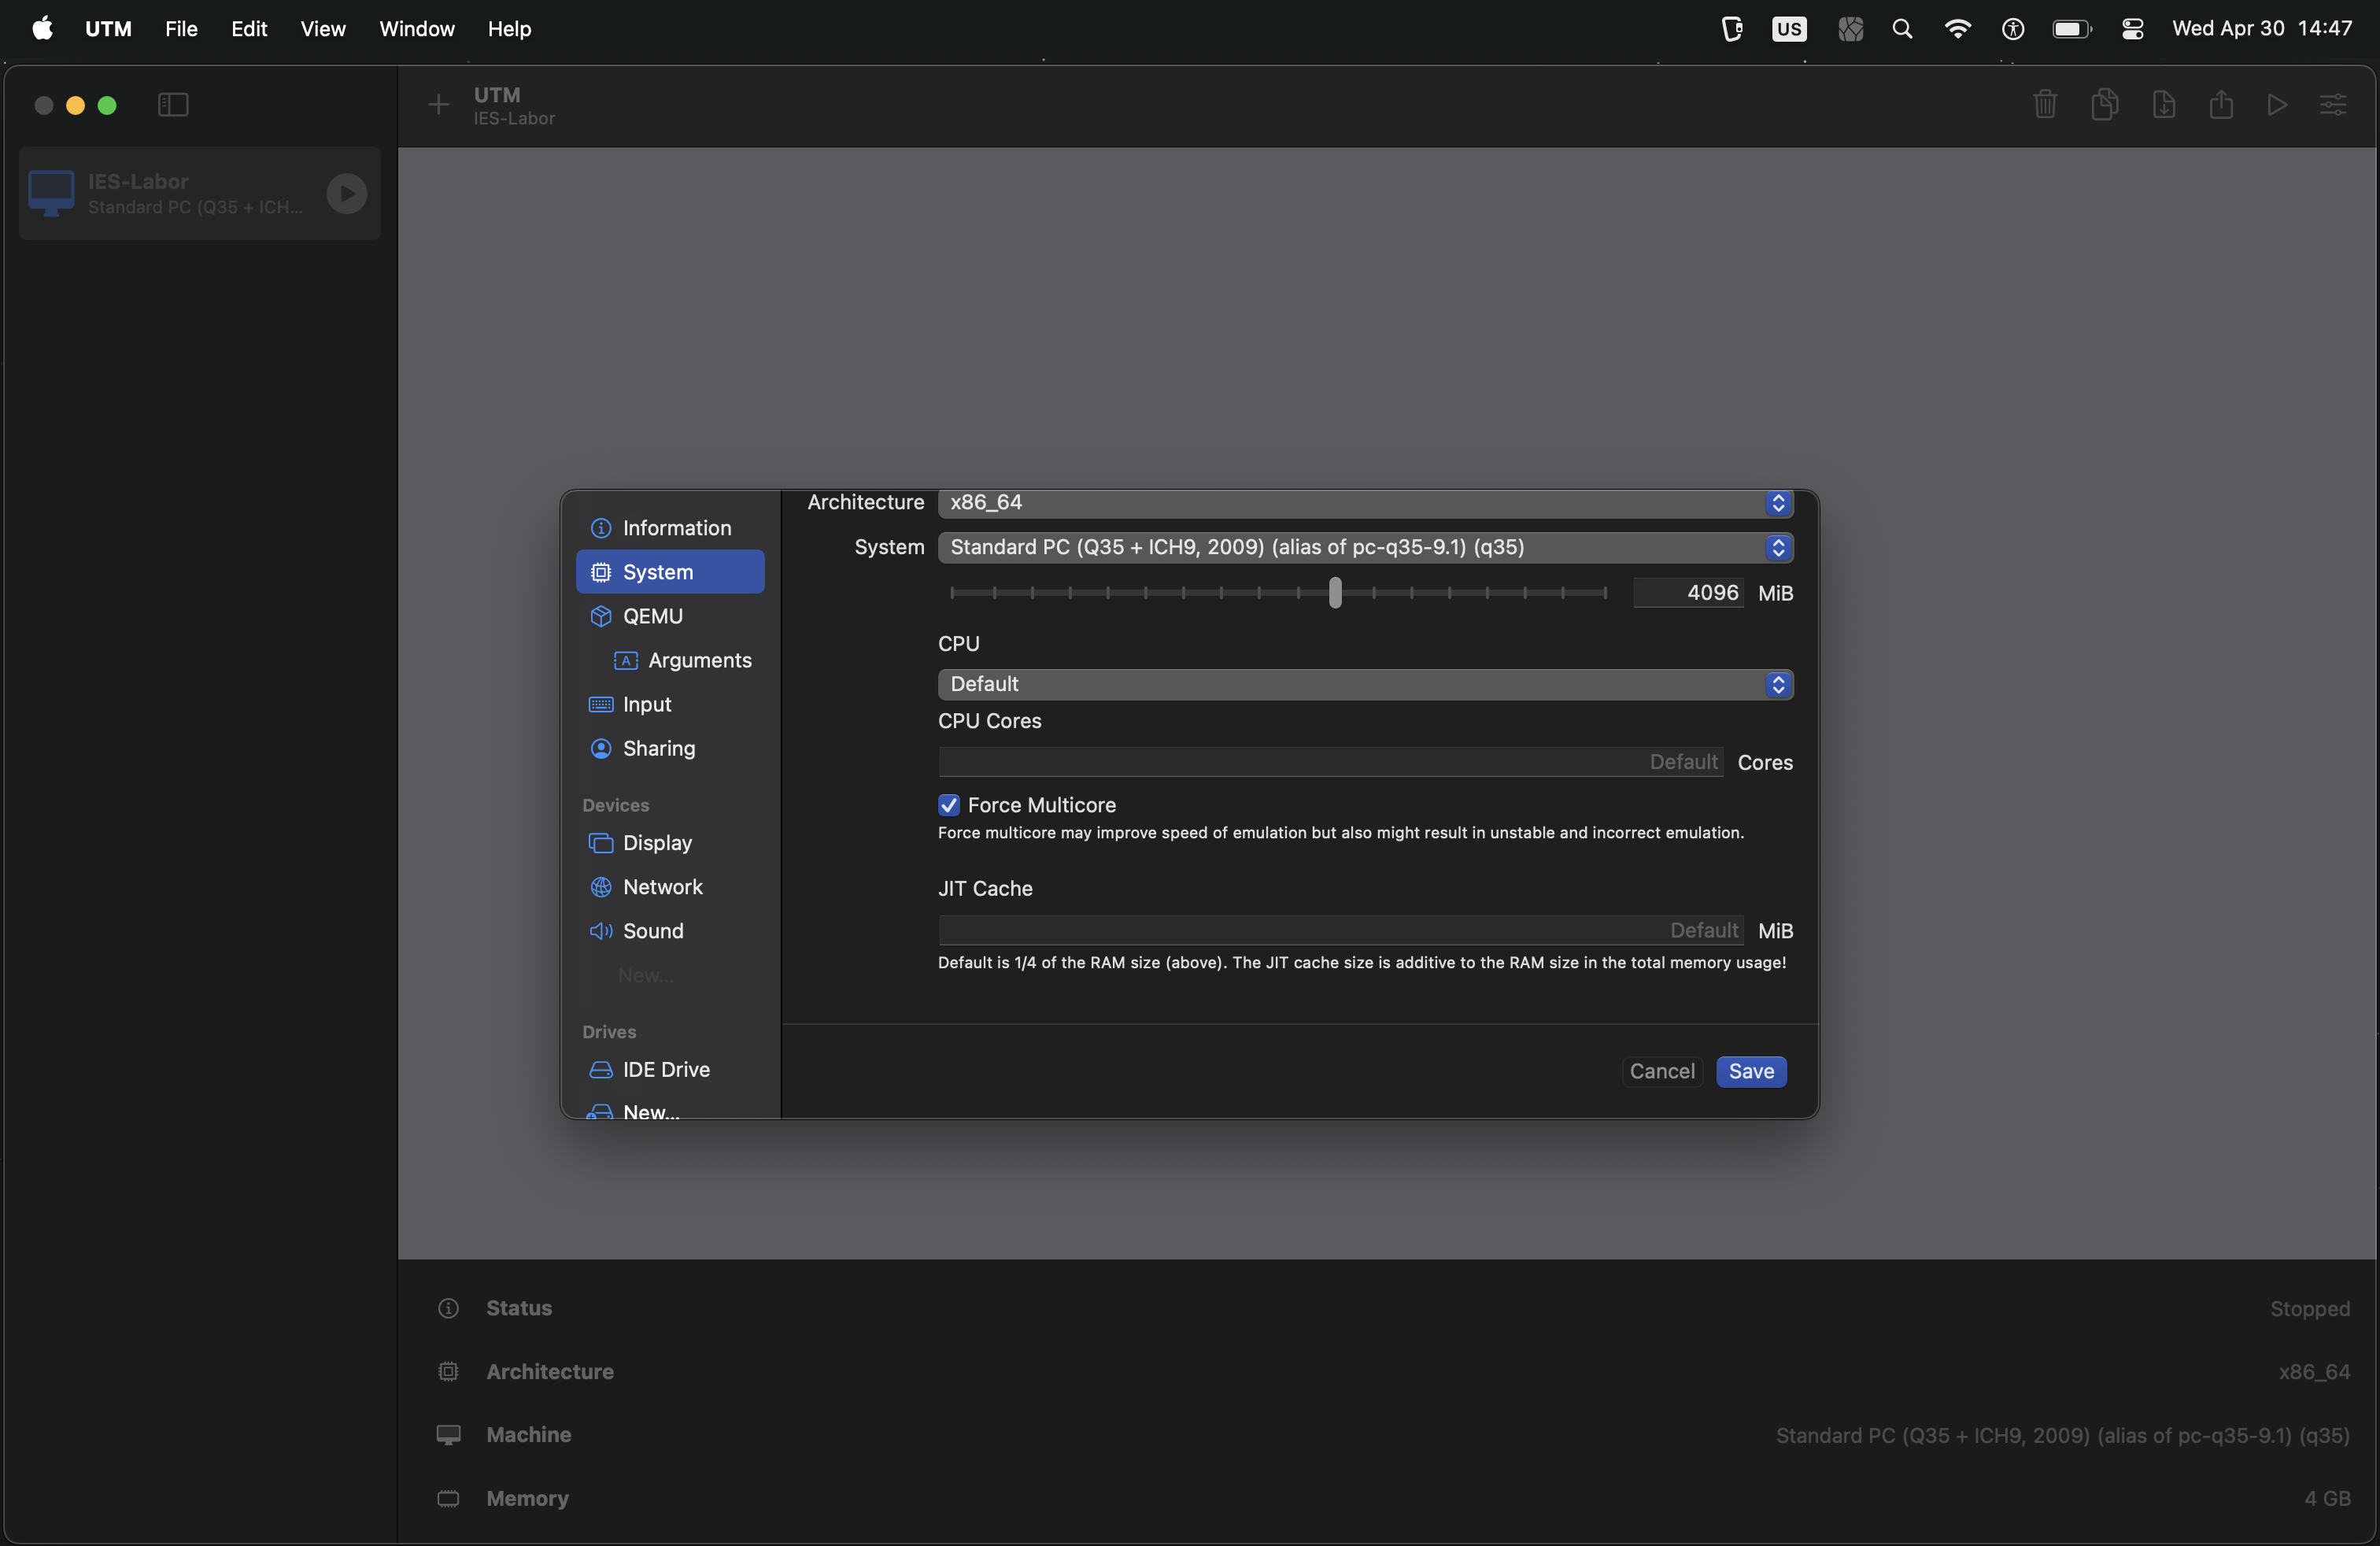
\includegraphics[width=0.48\textwidth]{images/img_utm_system-force-multicore.png}
    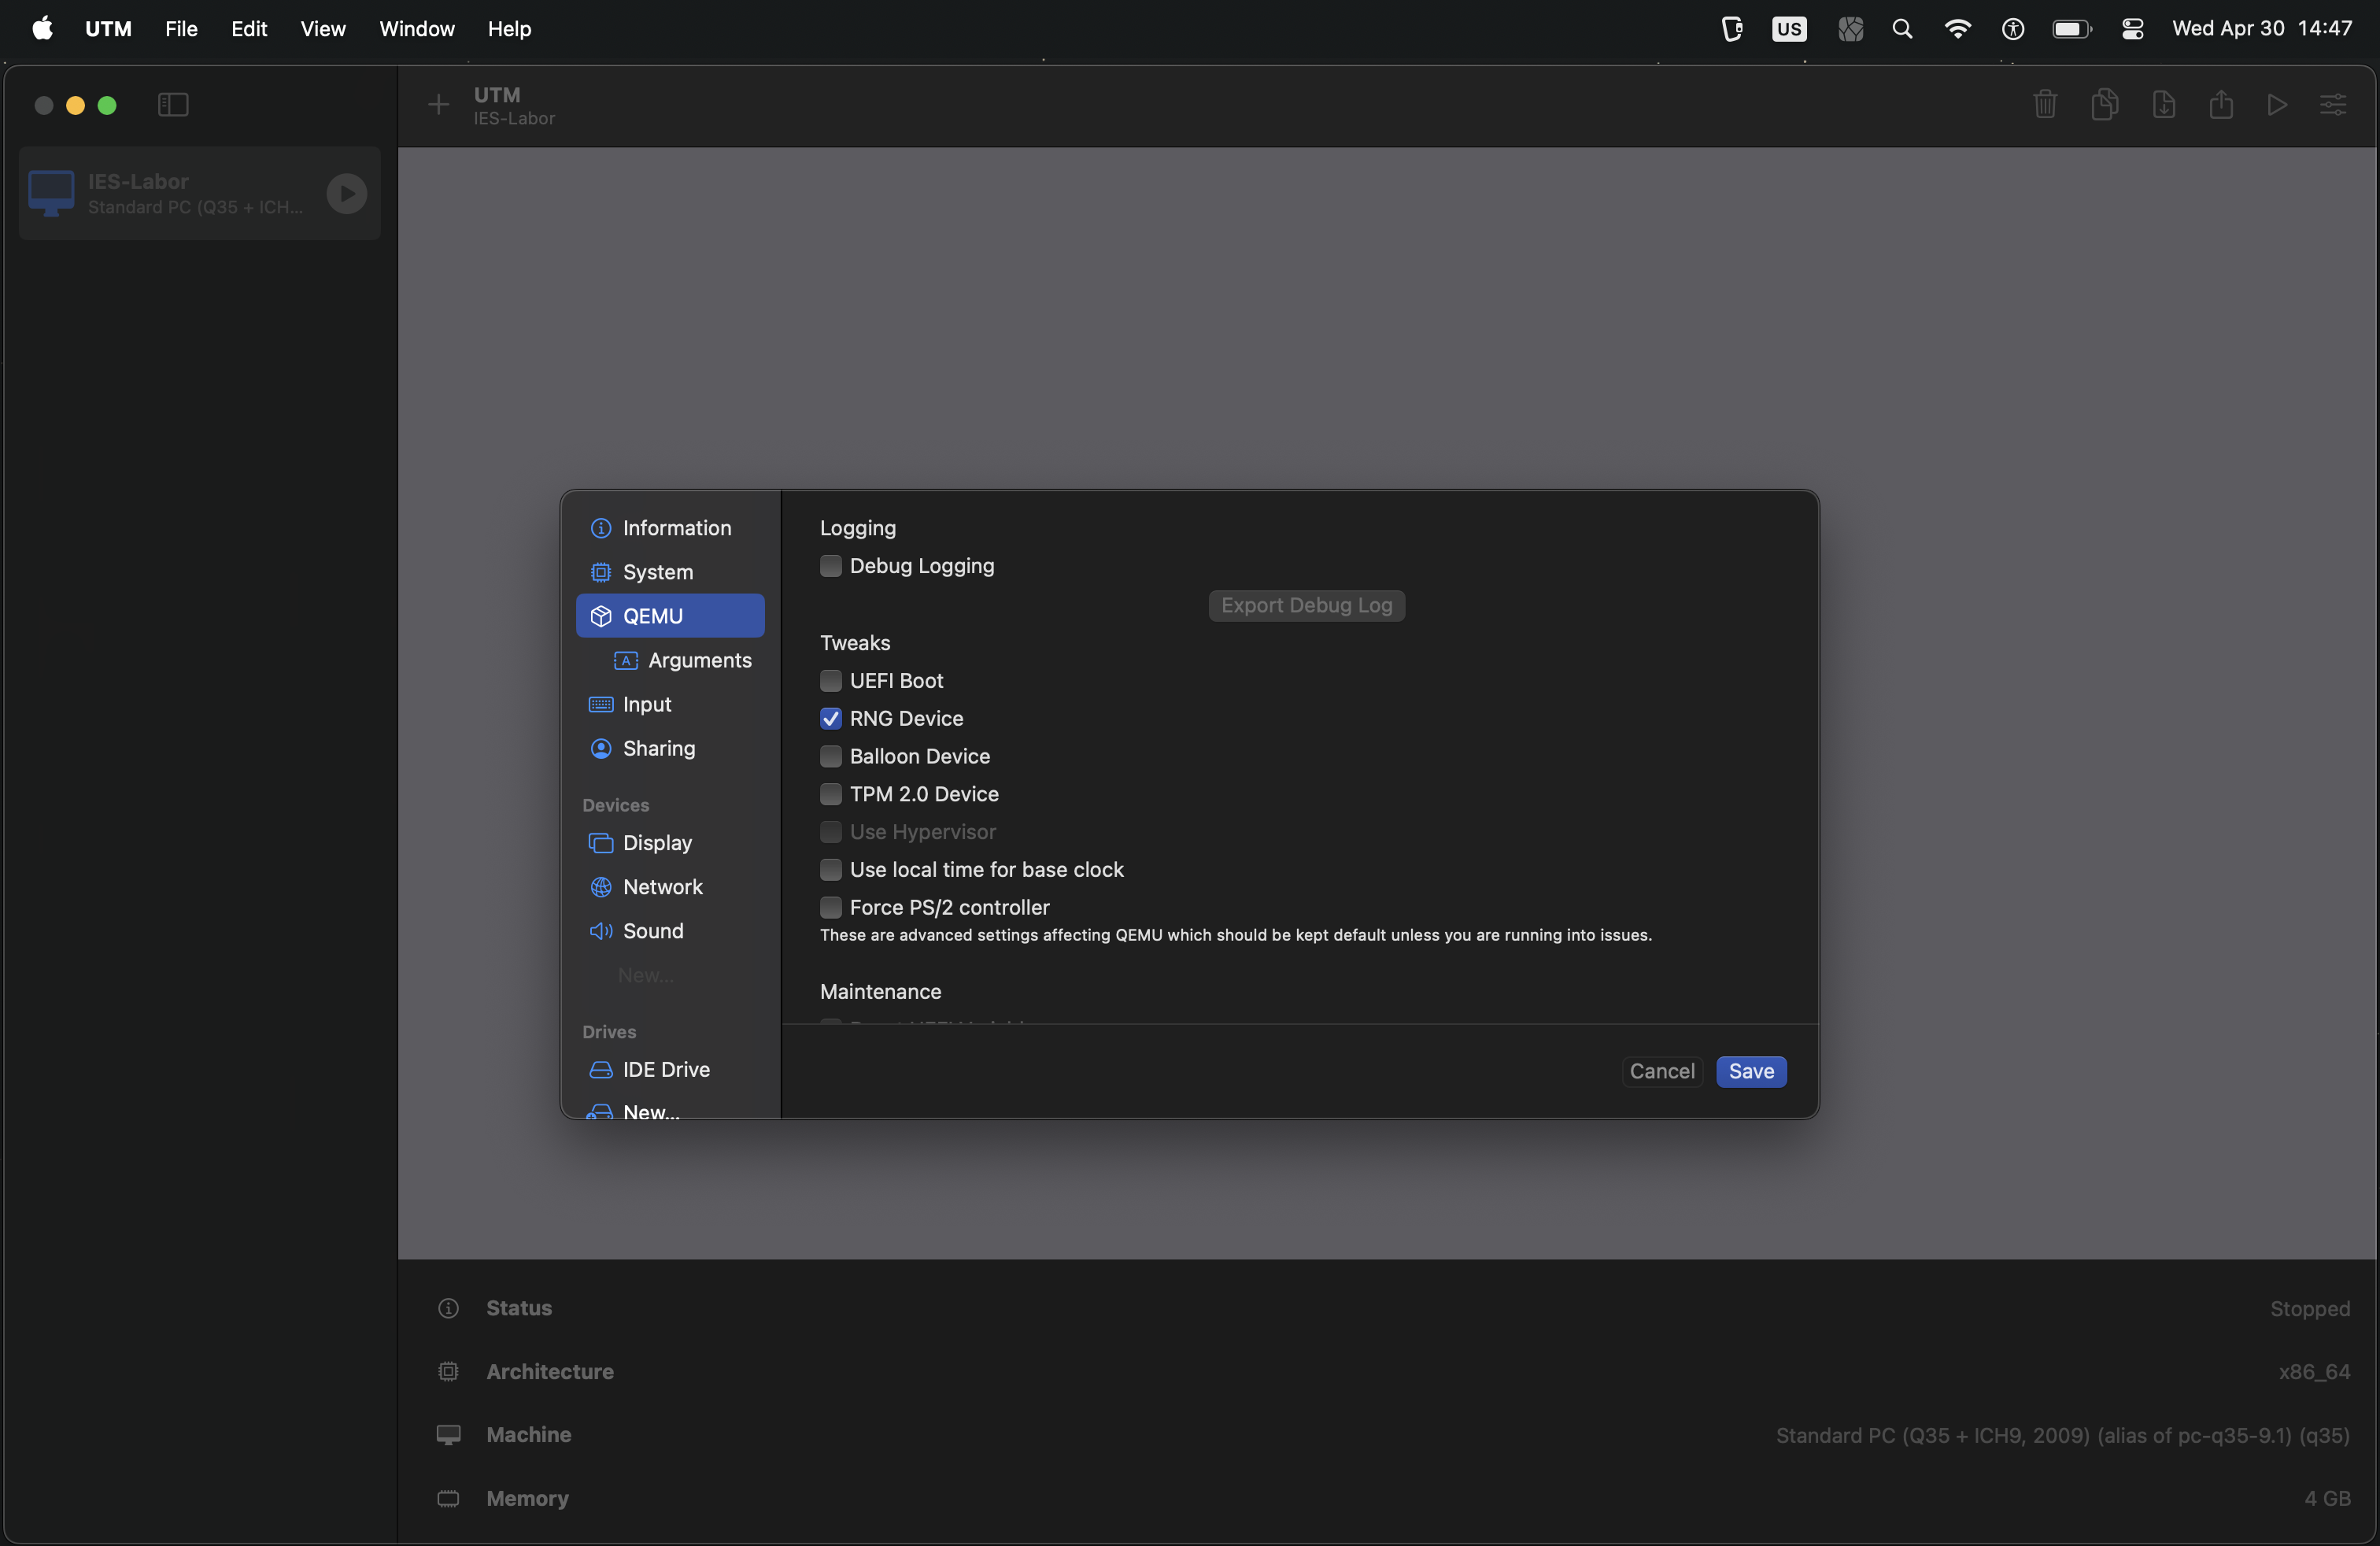
\includegraphics[width=0.48\textwidth]{images/img_utm_qemu-disable-uefi.png}
    \caption{System- und QEMU-Einstellungen}
    \label{fig:system-qemu}
\end{figure}

Die Änderungen gemäß Schritt 2-3 sind in Abbildung \ref{fig:system-qemu} dargestellt.

\begin{enumerate}[label=\arabic*.,leftmargin=1.5em,itemsep=0.3em,start=4]
  \item Setzen Sie unter Sharing den \emph{Directory share mode} auf \textbf{SPICE WebDAV}
\end{enumerate}

\begin{figure}[H]
    \centering
    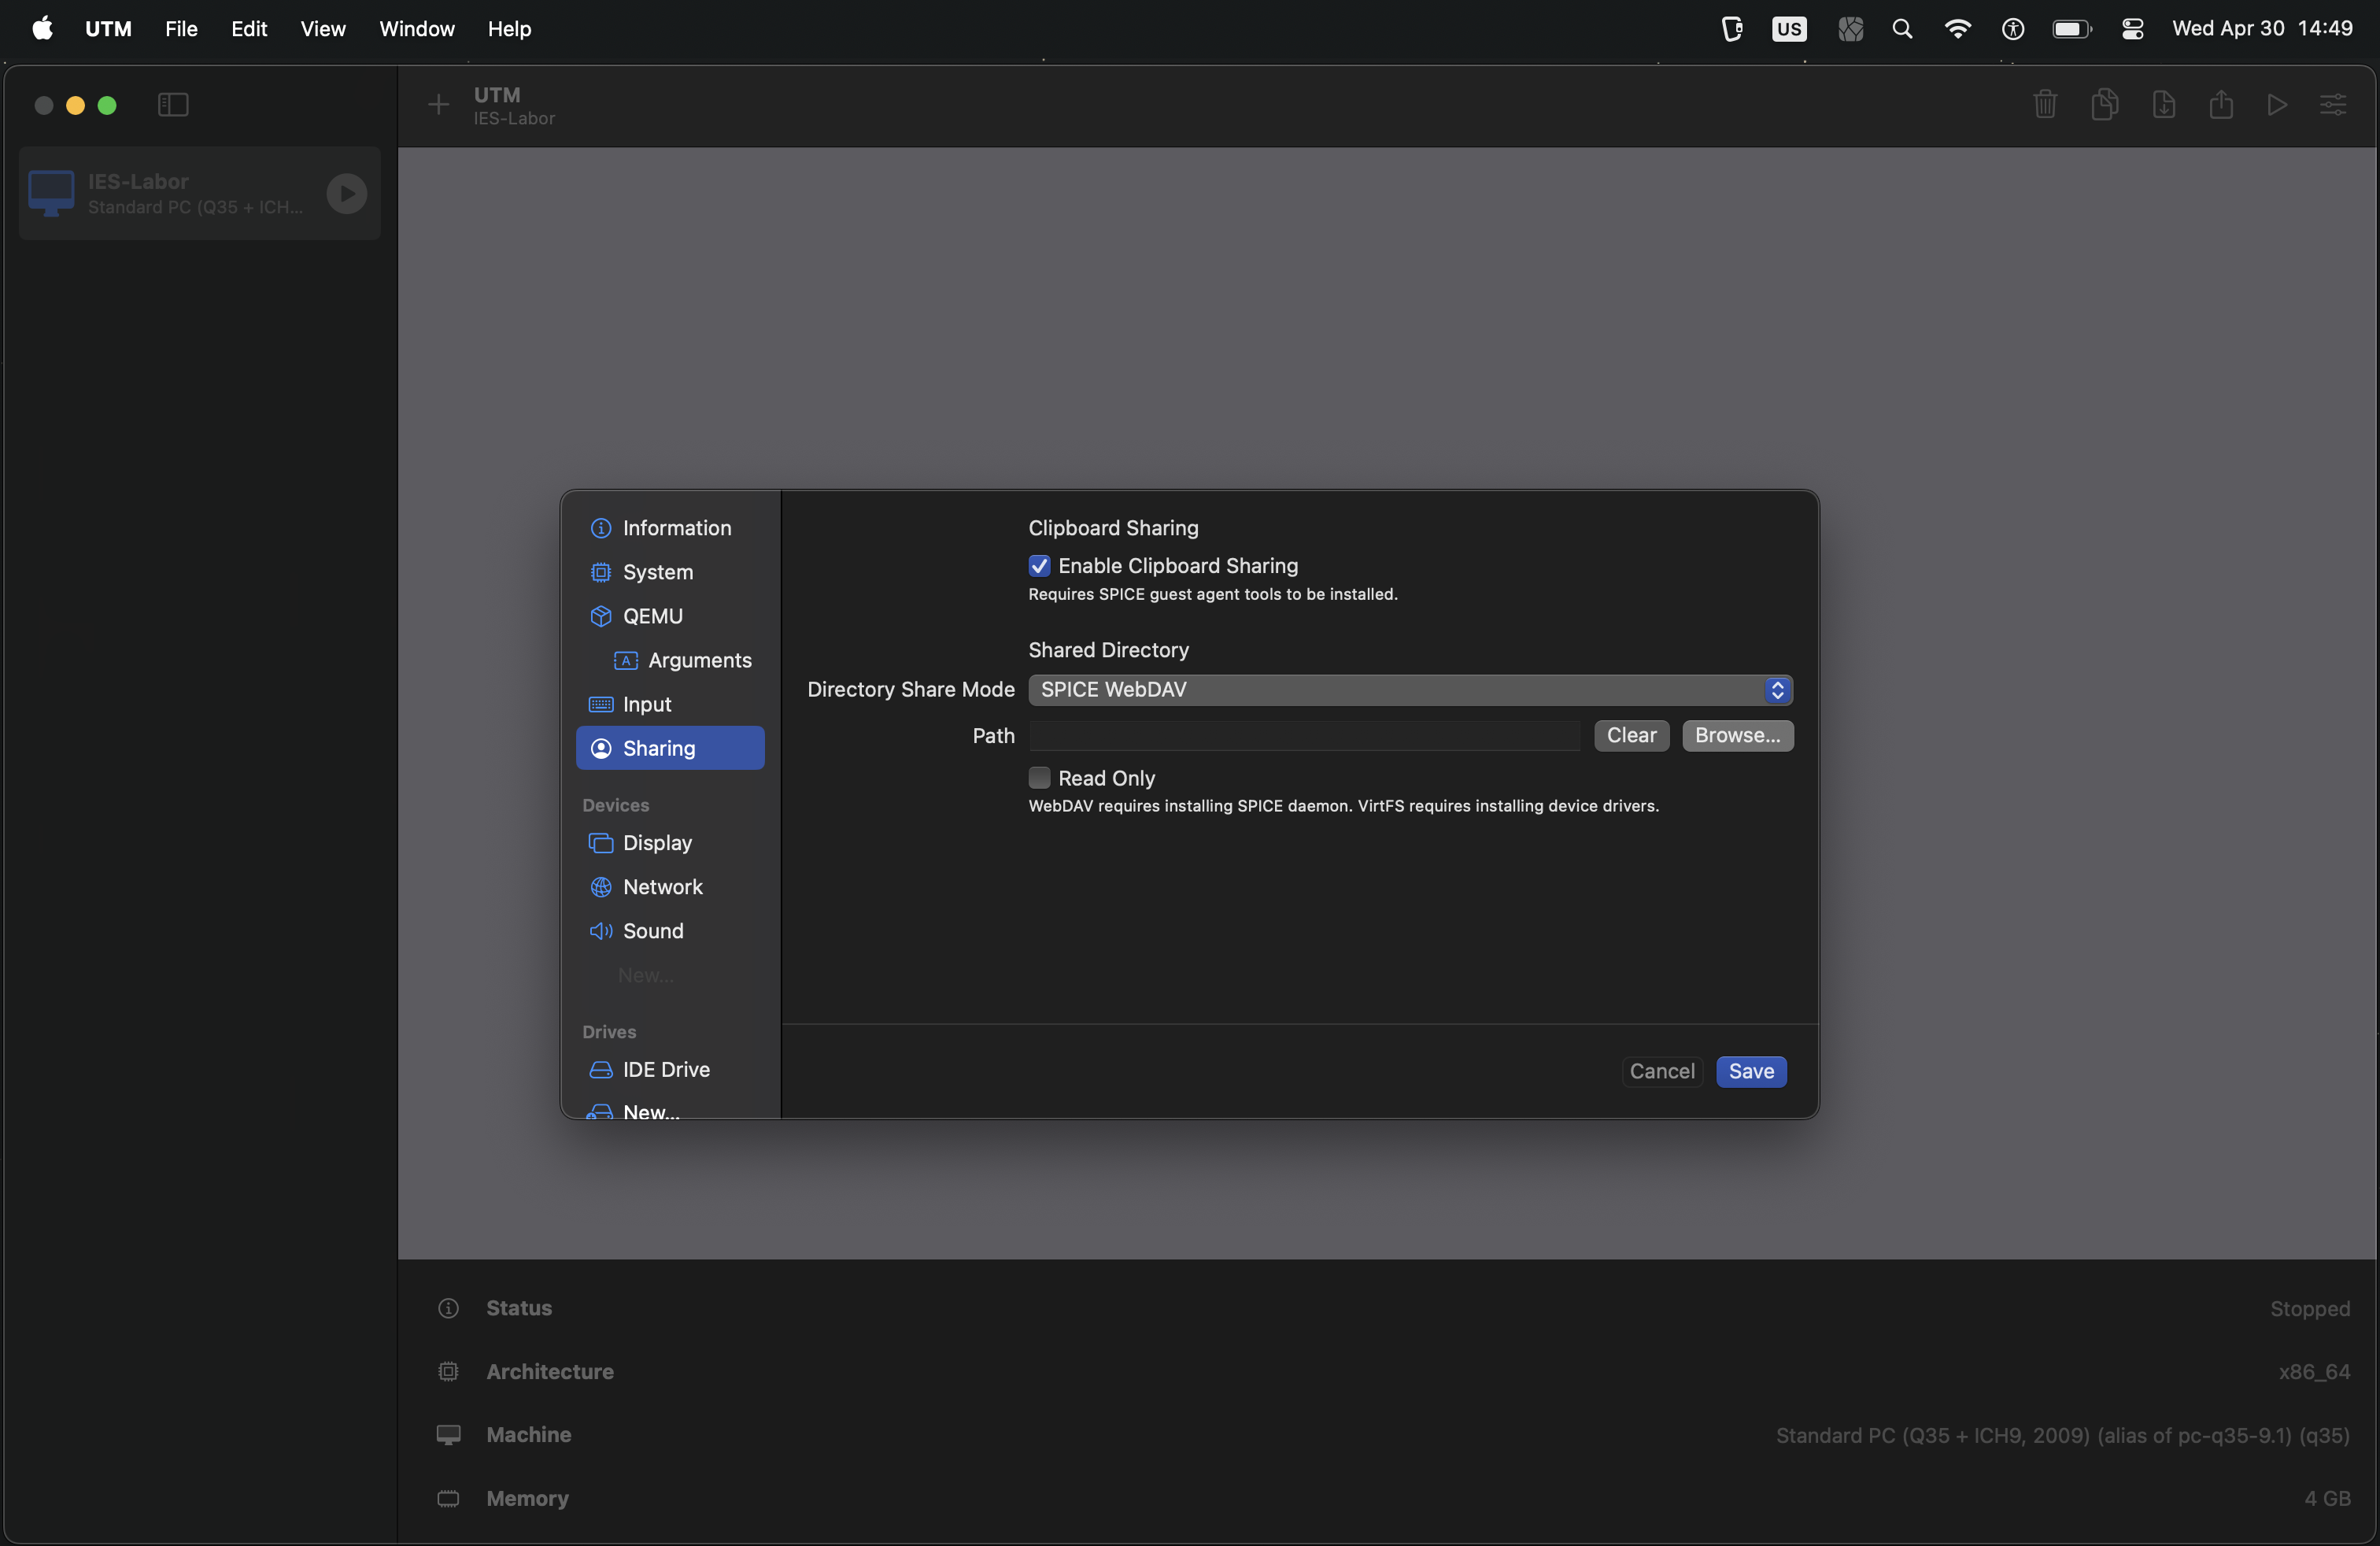
\includegraphics[width=0.7\textwidth]{images/img_utm_sharing.png}
    \caption{Sharing-Einstellungen}
    \label{fig:sharing}
\end{figure}

Die Einstellung aus Schritt 4 ist in Abbildung \ref{fig:sharing} zu sehen.

\begin{enumerate}[label=\arabic*.,leftmargin=1.5em,itemsep=0.3em,start=5]
	\item Klicken Sie bei Path auf \emph{Browse...} und wählen Sie einen neuen Ordner aus (dieser muss vorher erstellt werden)
\end{enumerate}

\begin{figure}[H]
    \centering
    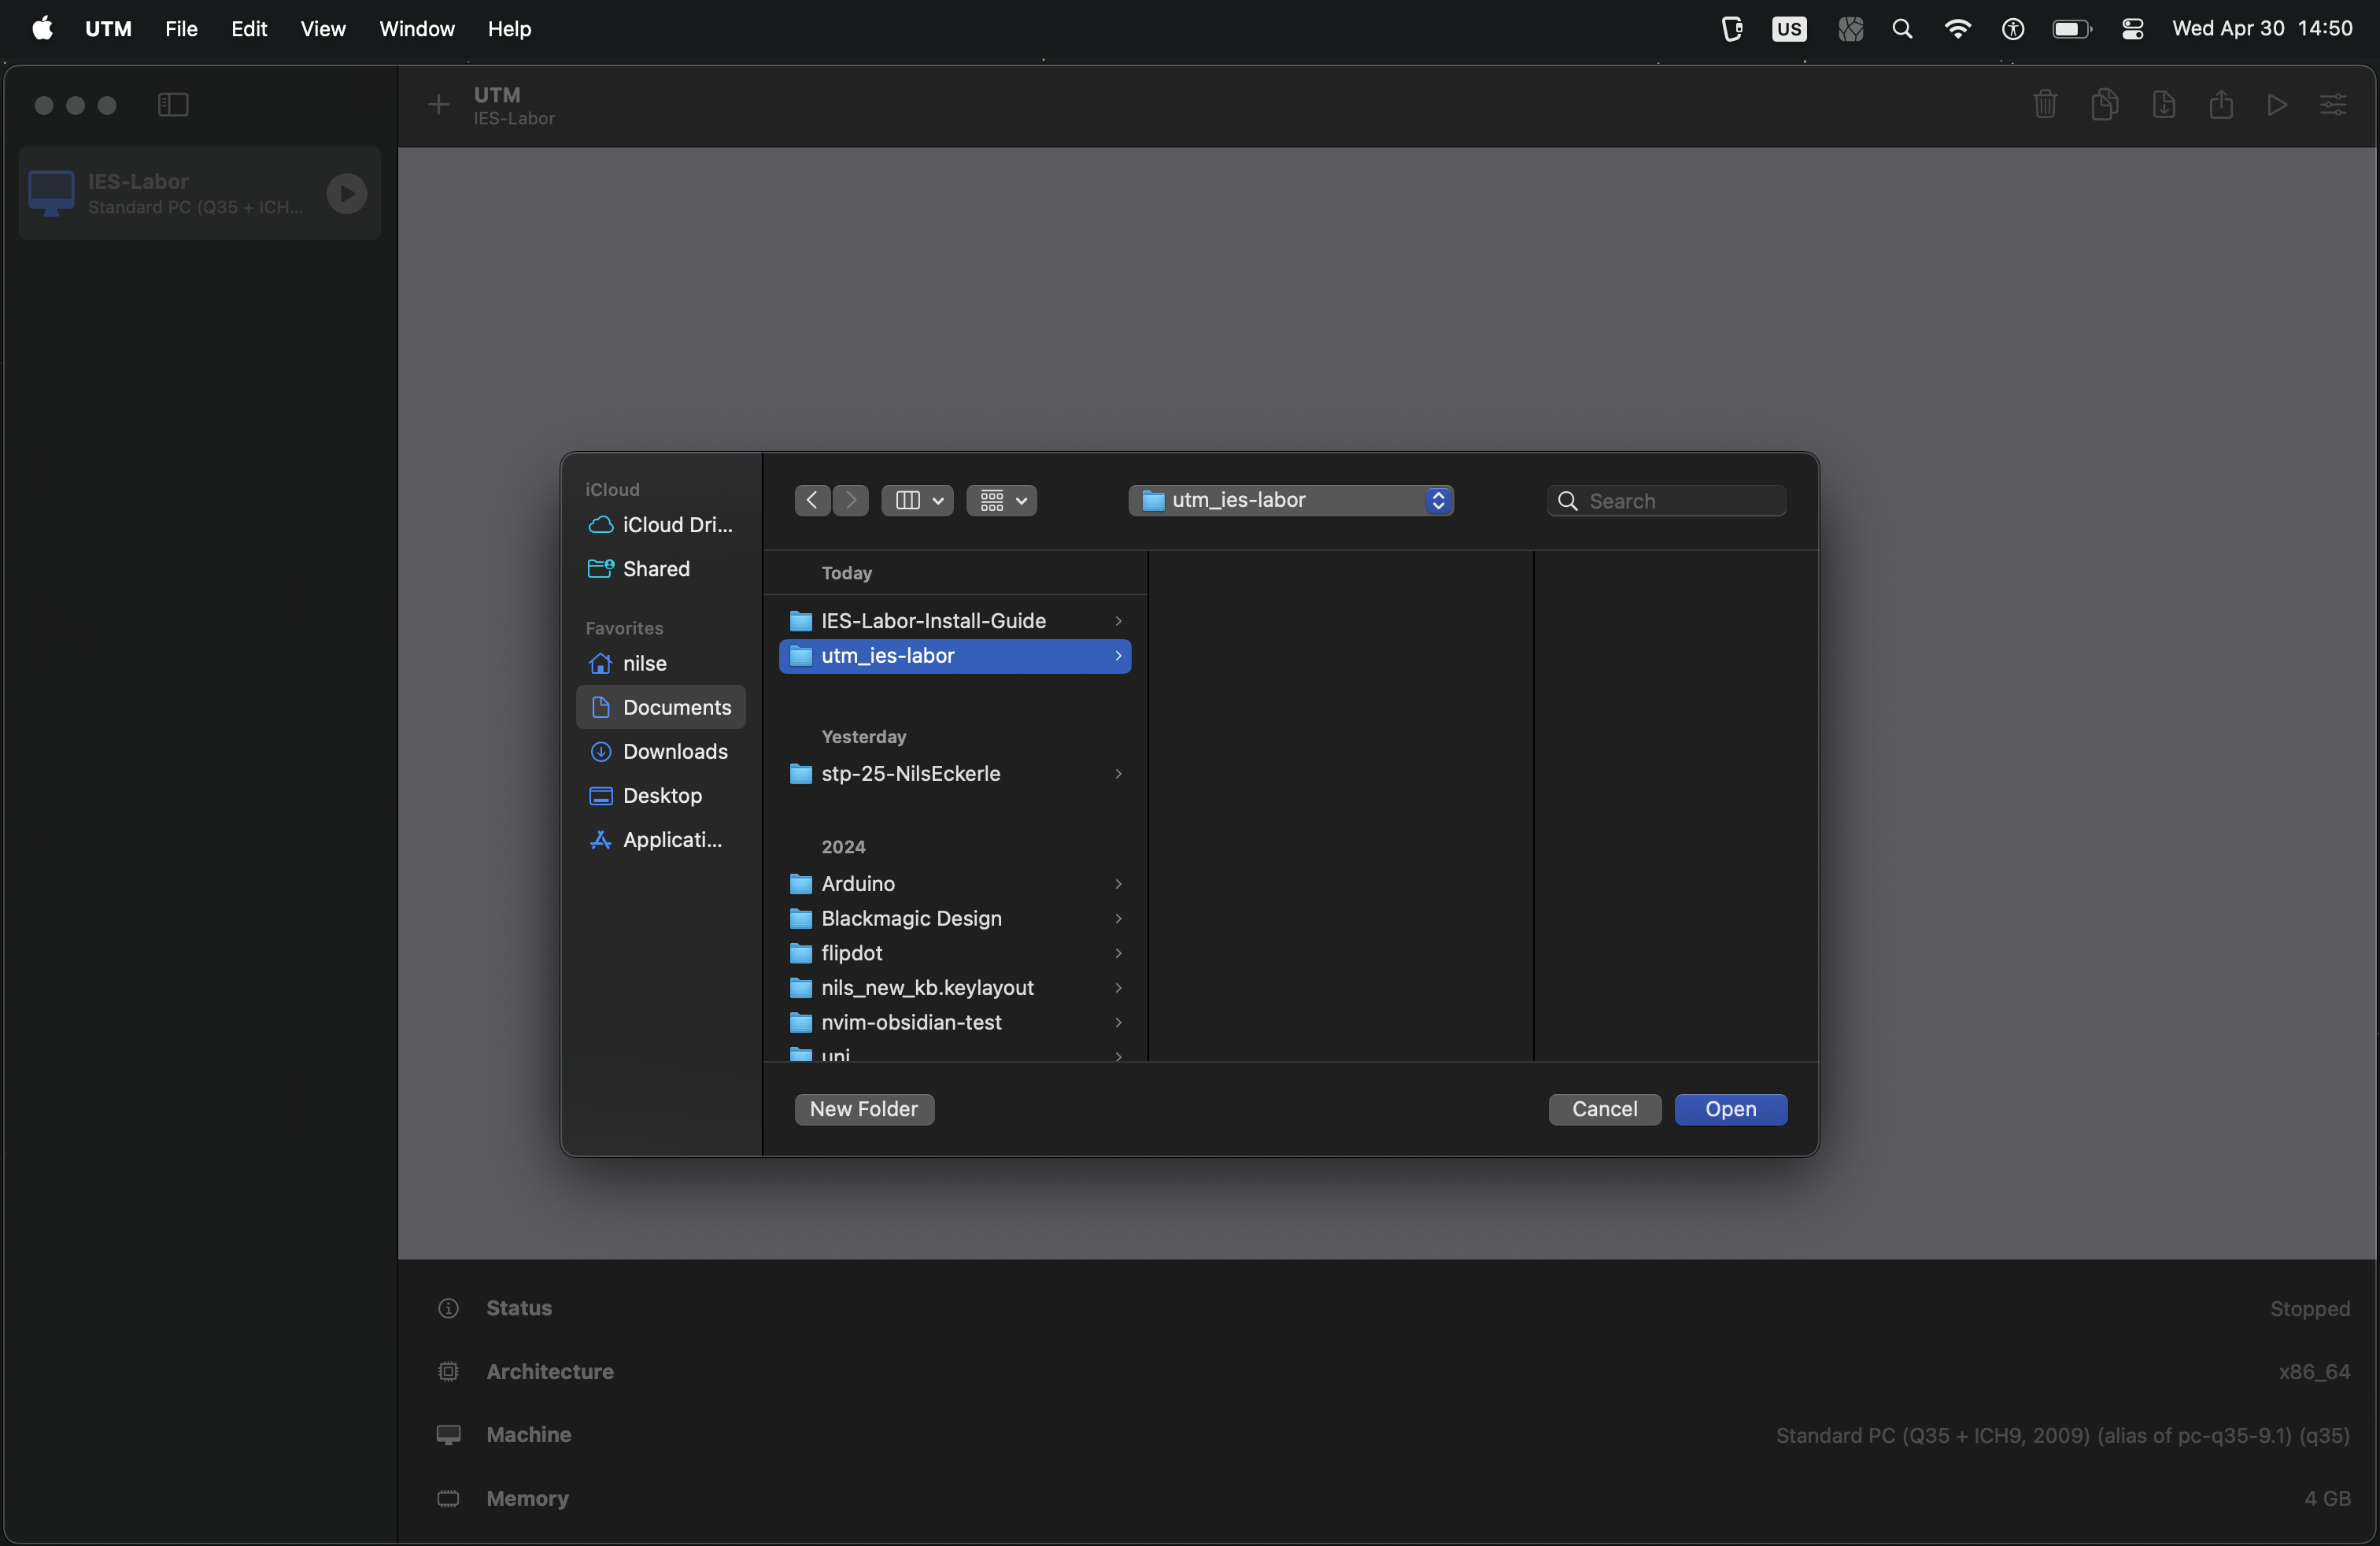
\includegraphics[width=0.7\textwidth]{images/img_utm_sharing-new-shared-directory.png}
    \caption{Auswahl eines Shared Directory}
    \label{fig:shared-directory}
\end{figure}

Die Auswahl eines Shared Directory gemäß Schritt 5 ist in Abbildung \ref{fig:shared-directory} dargestellt.

\begin{enumerate}[label=\arabic*.,leftmargin=1.5em,itemsep=0.3em,start=6]
  \item Wählen Sie unter Display:
  \begin{itemize}[leftmargin=1.5em]
    \item Emulated display card: \textbf{VGA}
    \item VGA device RAM (MB): mindestens \textbf{128 MB}
  \end{itemize}
\end{enumerate}

\begin{figure}[H]
    \centering
    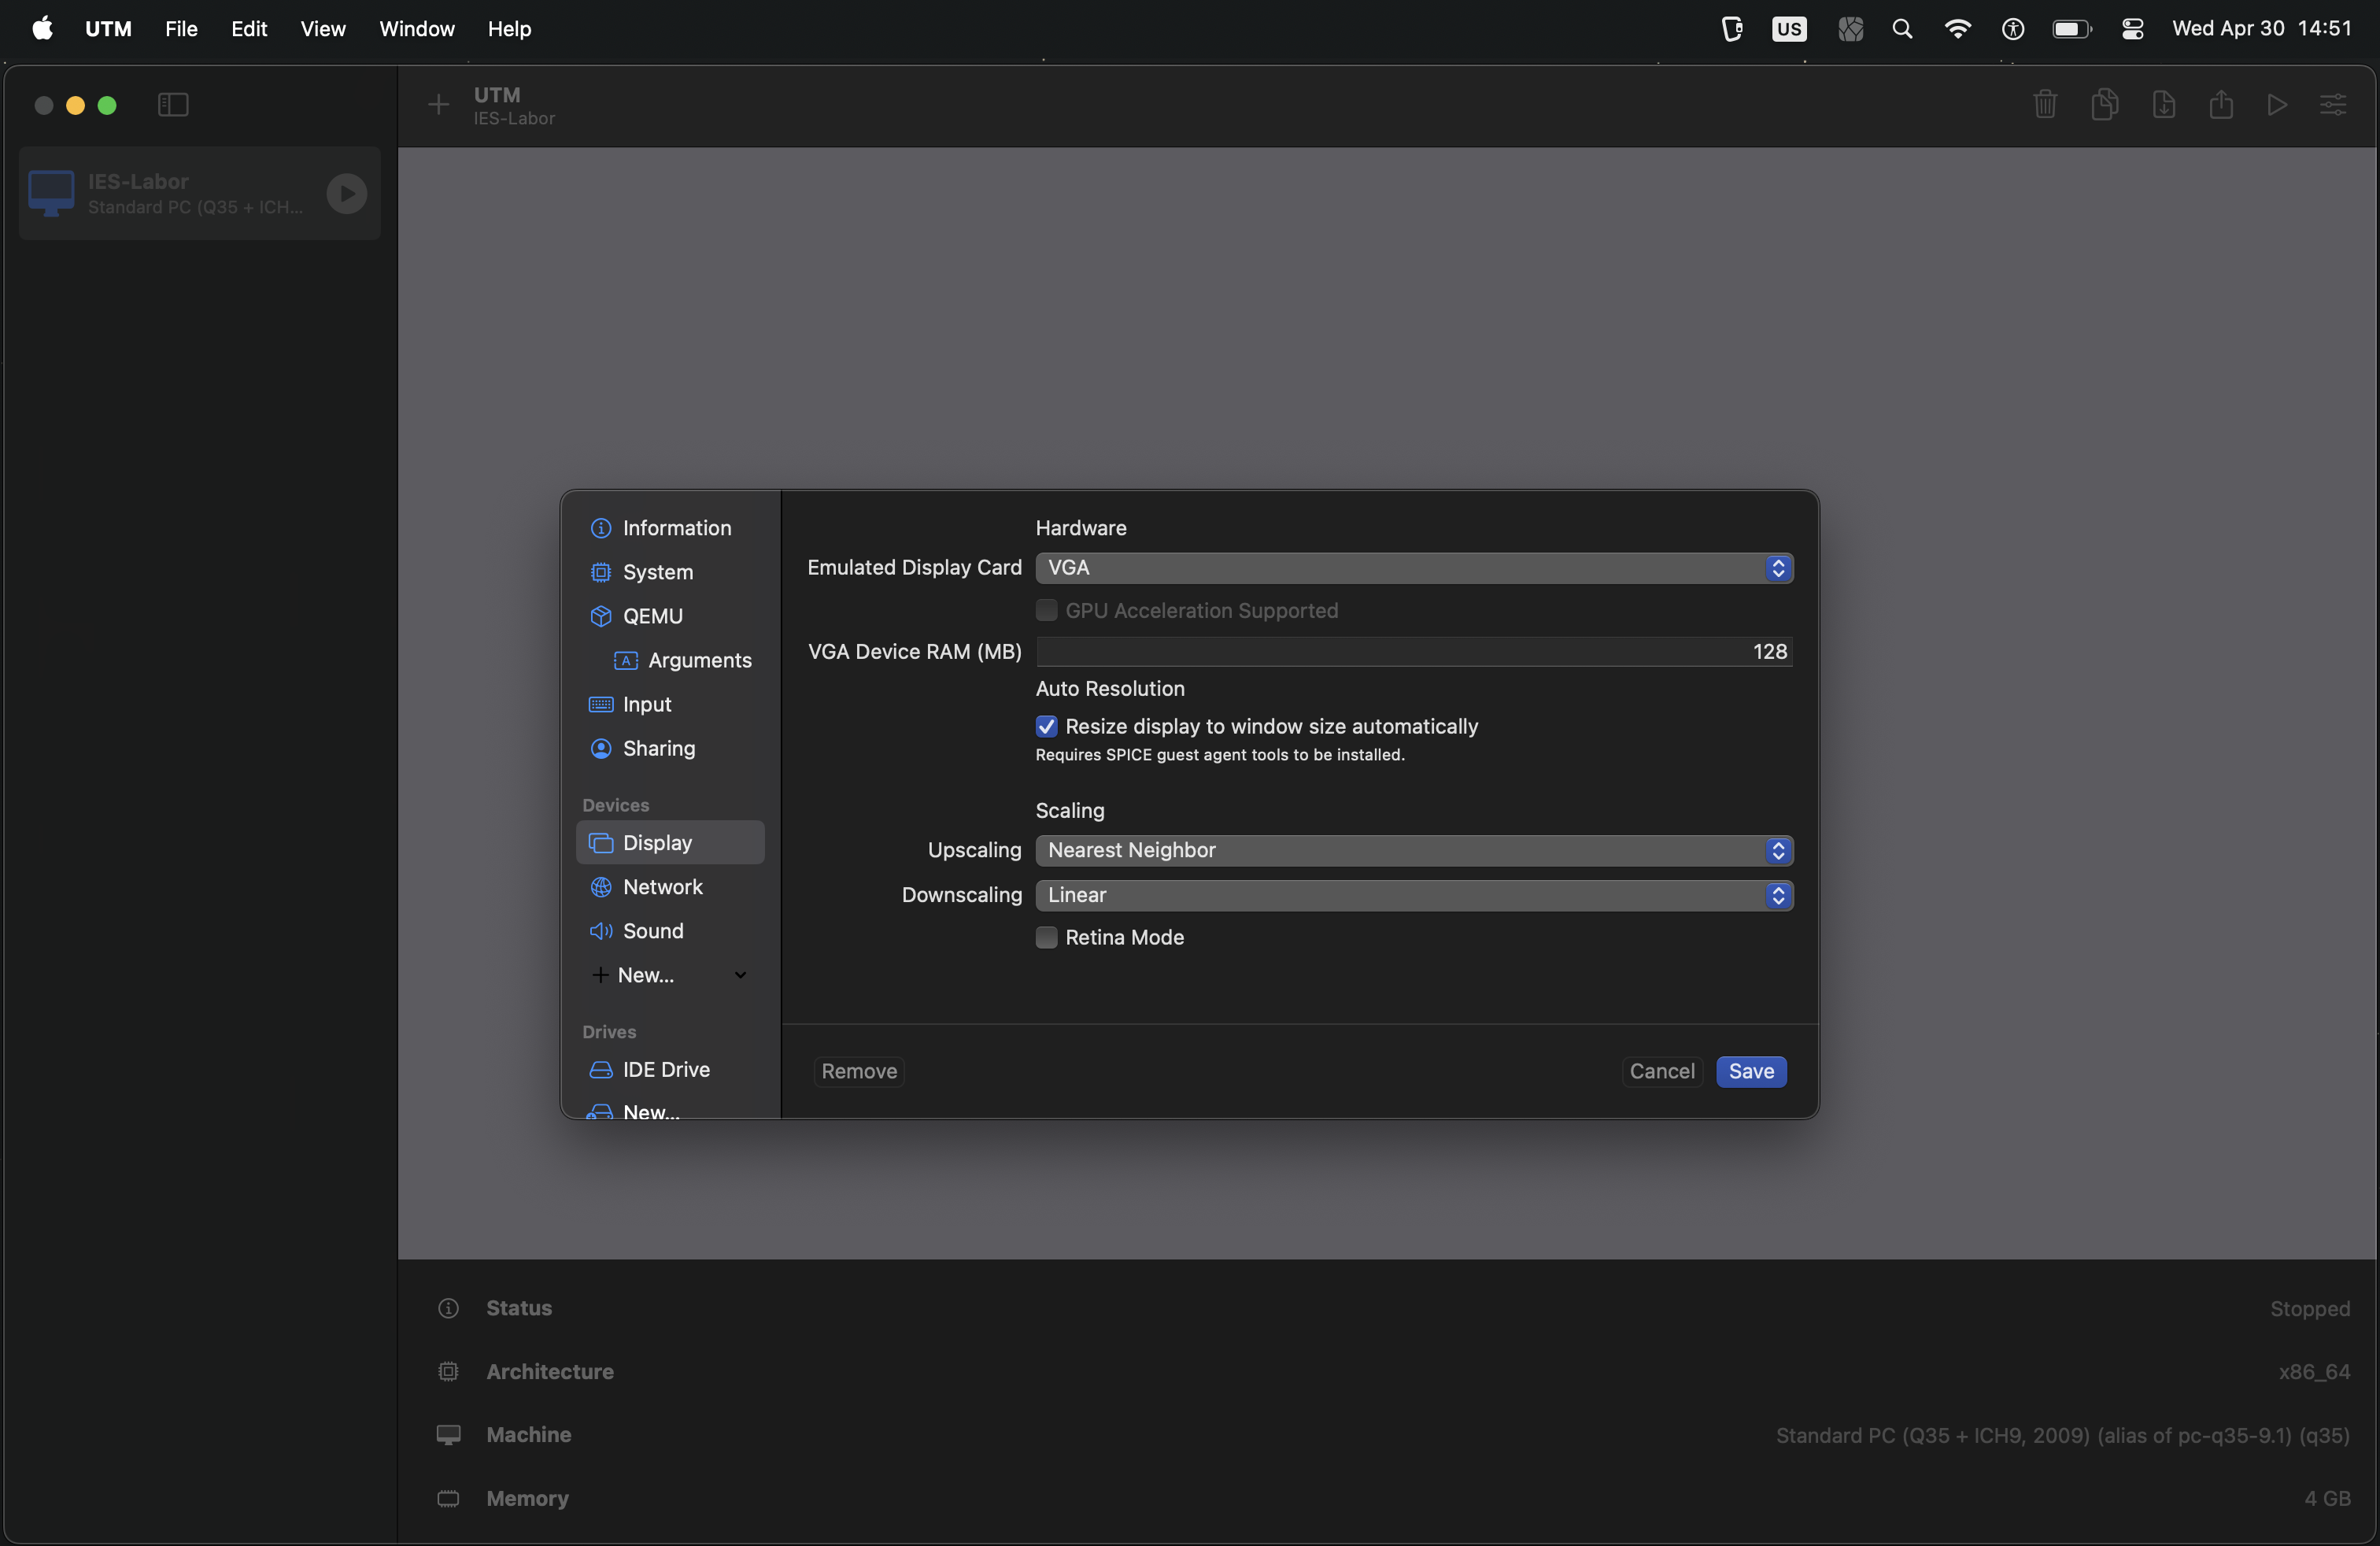
\includegraphics[width=0.7\textwidth]{images/img_utm_display.png}
    \caption{Display-Einstellungen}
    \label{fig:display}
\end{figure}

Die Display-Einstellungen aus Schritt 6 sind in Abbildung \ref{fig:display} zu sehen.

\begin{enumerate}[label=\arabic*.,leftmargin=1.5em,itemsep=0.3em,start=7]
  \item Konfigurieren Sie die Netzwerkeinstellungen exakt wie folgt:
  \begin{itemize}[leftmargin=1.5em]
    \item Network mode: \textbf{Emulate VLAN}
    \item Emulate Network Card: \textbf{Intel Gigabit Ethernet (e1000-82545em)}
    \item MAC Adresse: \textbf{08:00:27:4D:6E:A1}
  \end{itemize}
\end{enumerate}

\begin{figure}[H]
    \centering
    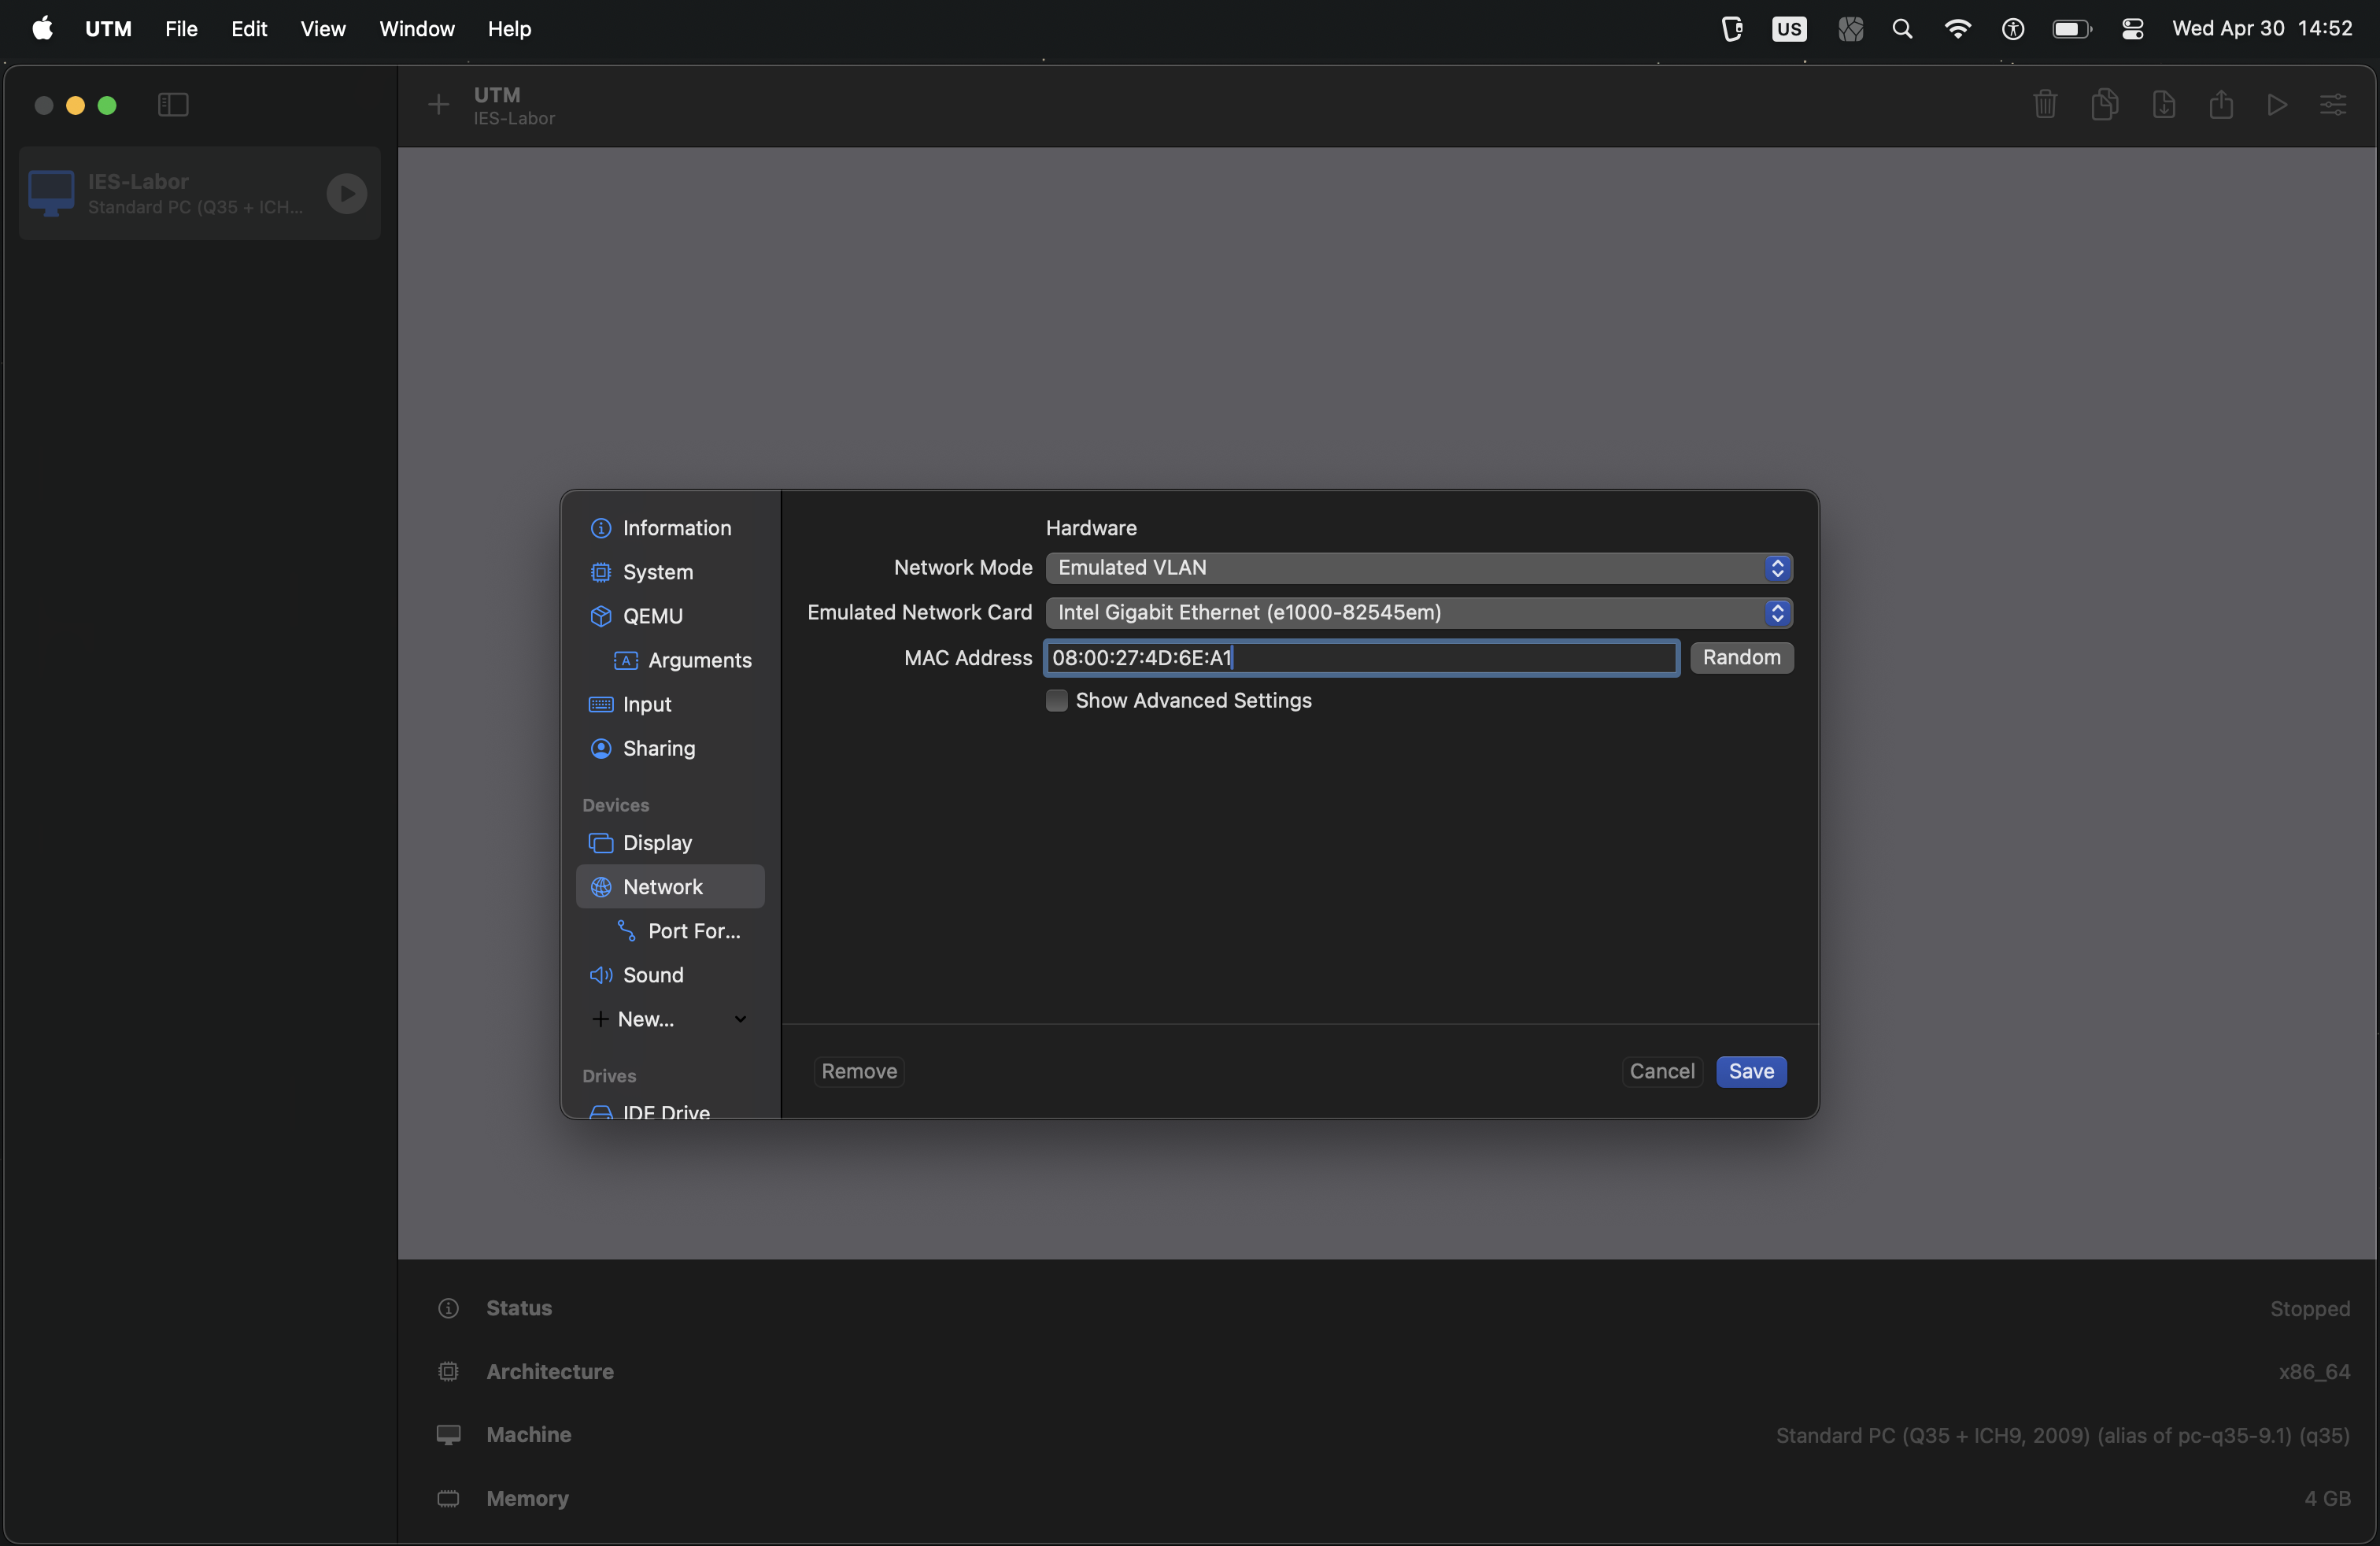
\includegraphics[width=0.7\textwidth]{images/img_utm_network.png}
    \caption{Netzwerkeinstellungen}
    \label{fig:network}
\end{figure}

Die Netzwerkkonfiguration gemäß Schritt 7 ist in Abbildung \ref{fig:network} dargestellt.

\begin{enumerate}[label=\arabic*.,leftmargin=1.5em,itemsep=0.3em,start=8]
  \item Löschen Sie die bestehende Disk
  \item Importieren Sie die neue Disk
\end{enumerate}

\begin{figure}[H]
    \centering
    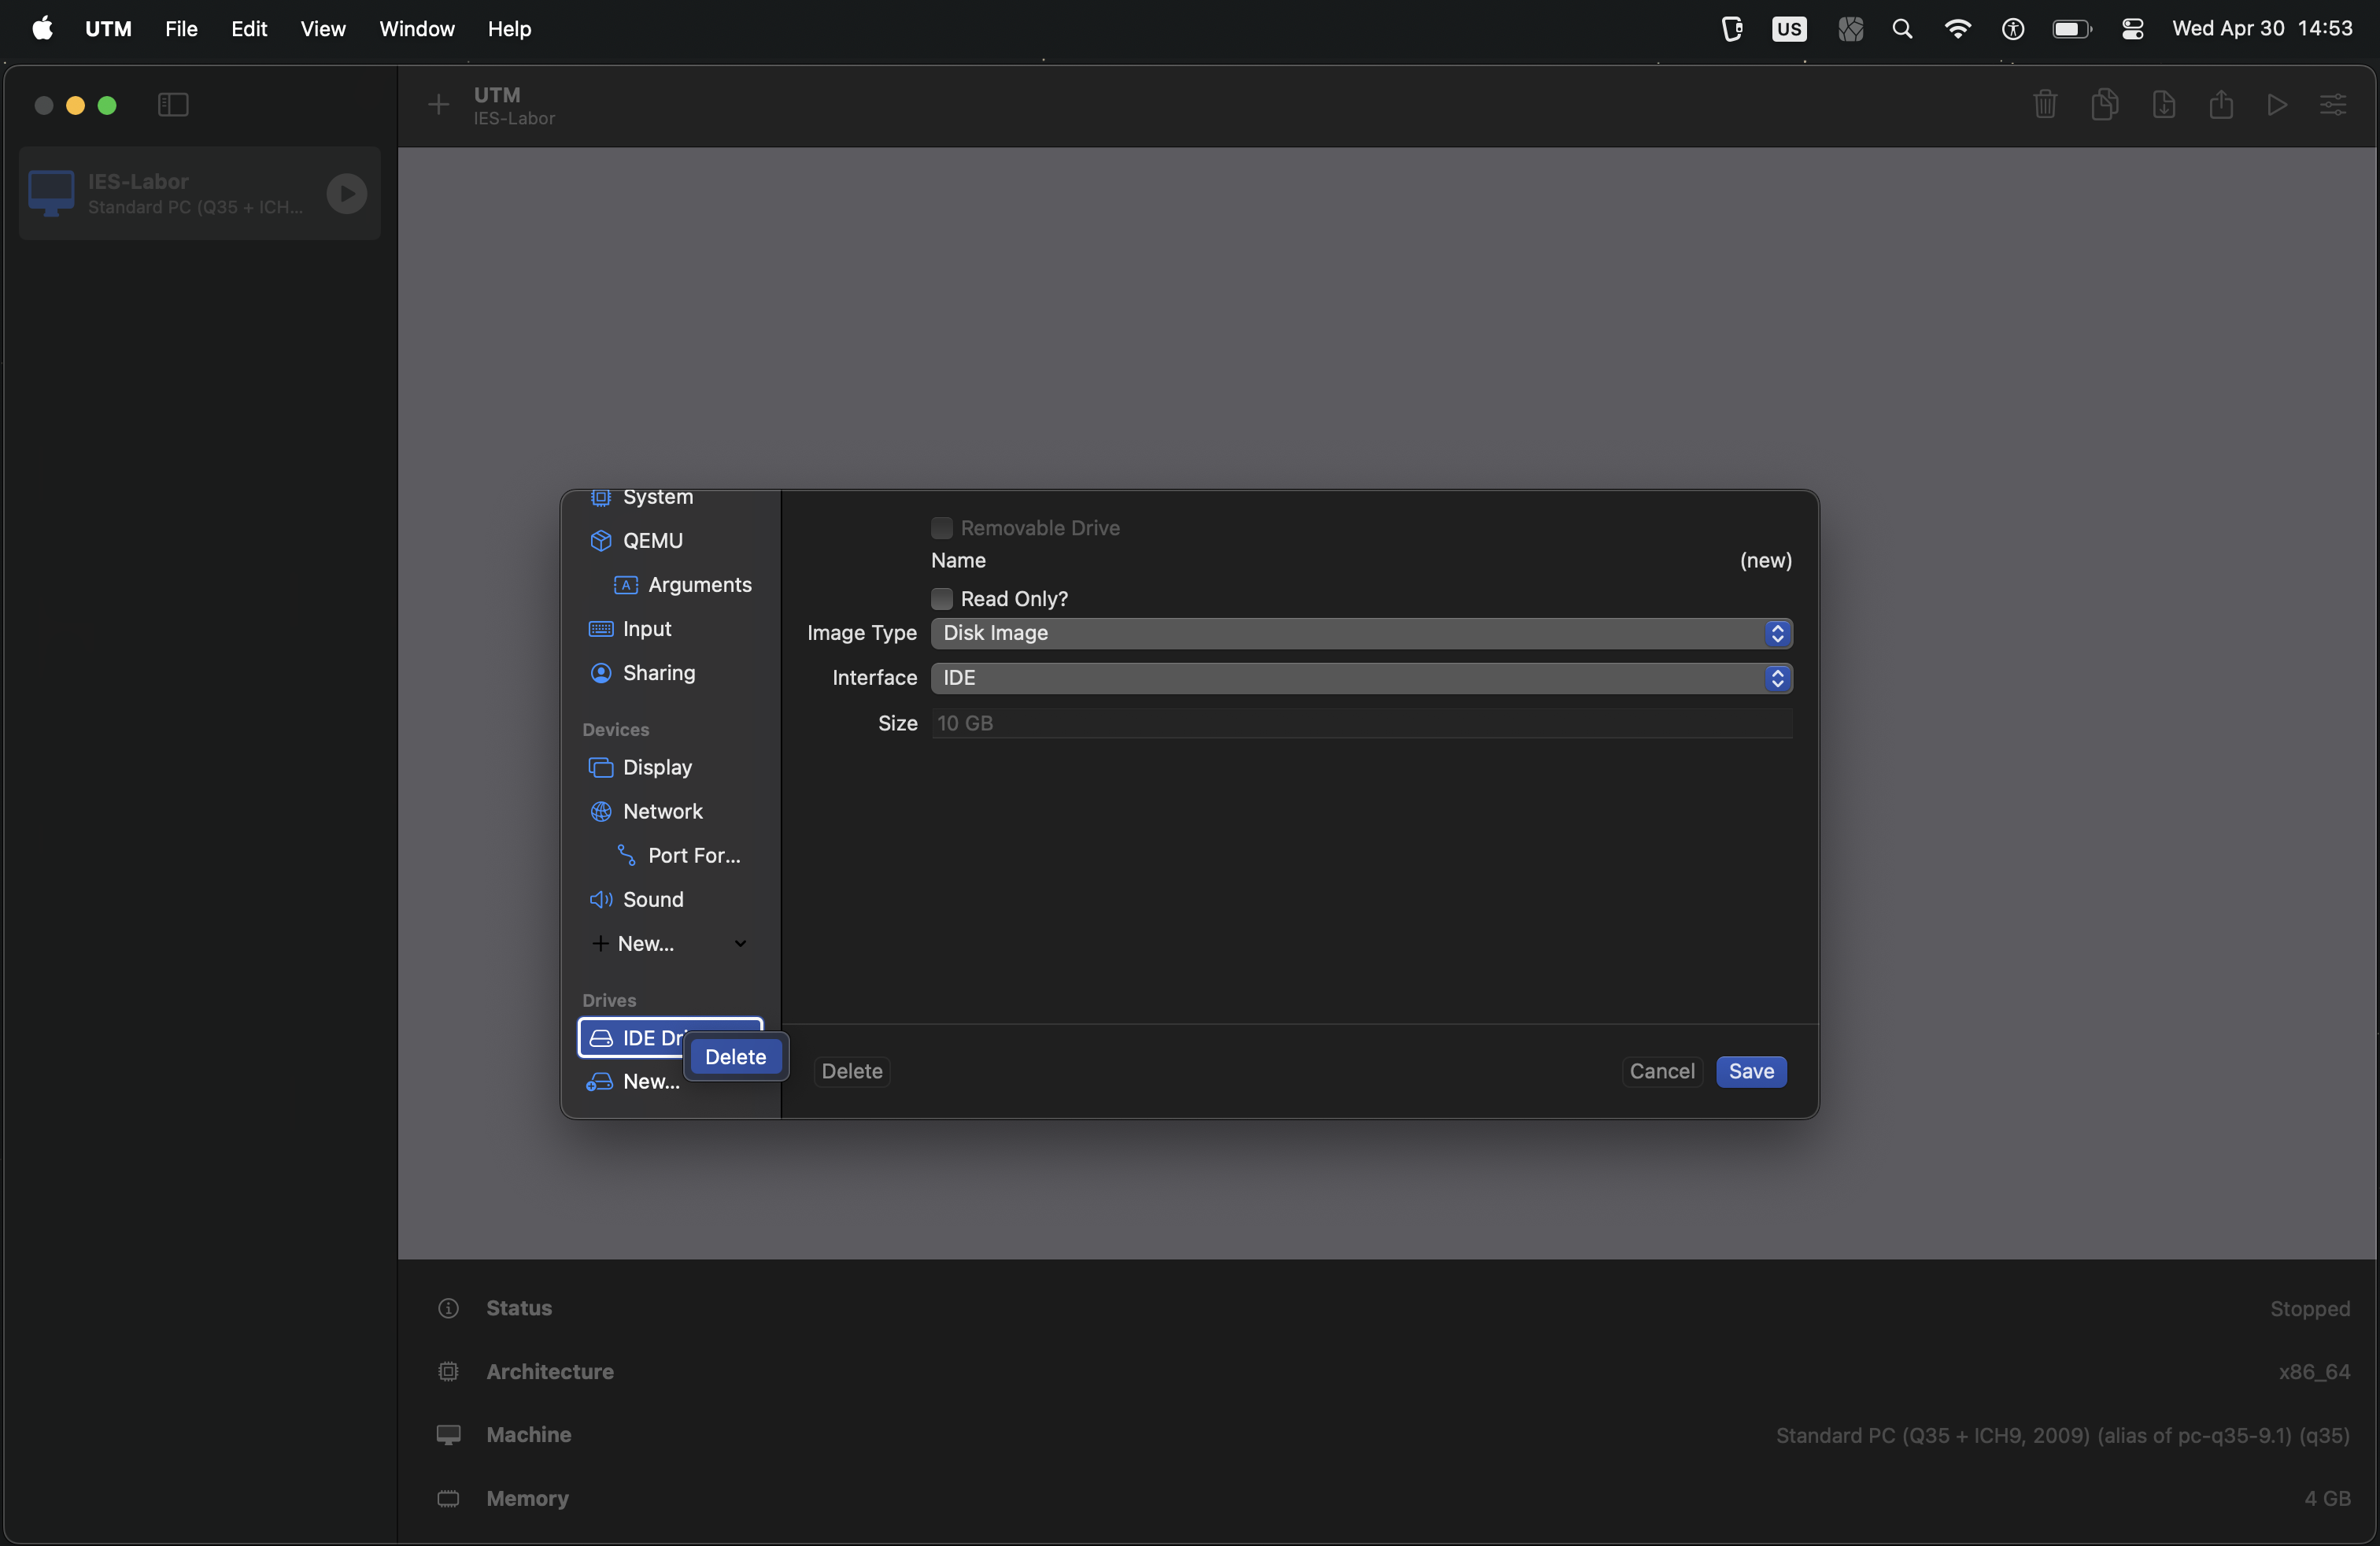
\includegraphics[width=0.48\textwidth]{images/img_utm_disk-delete.png}
    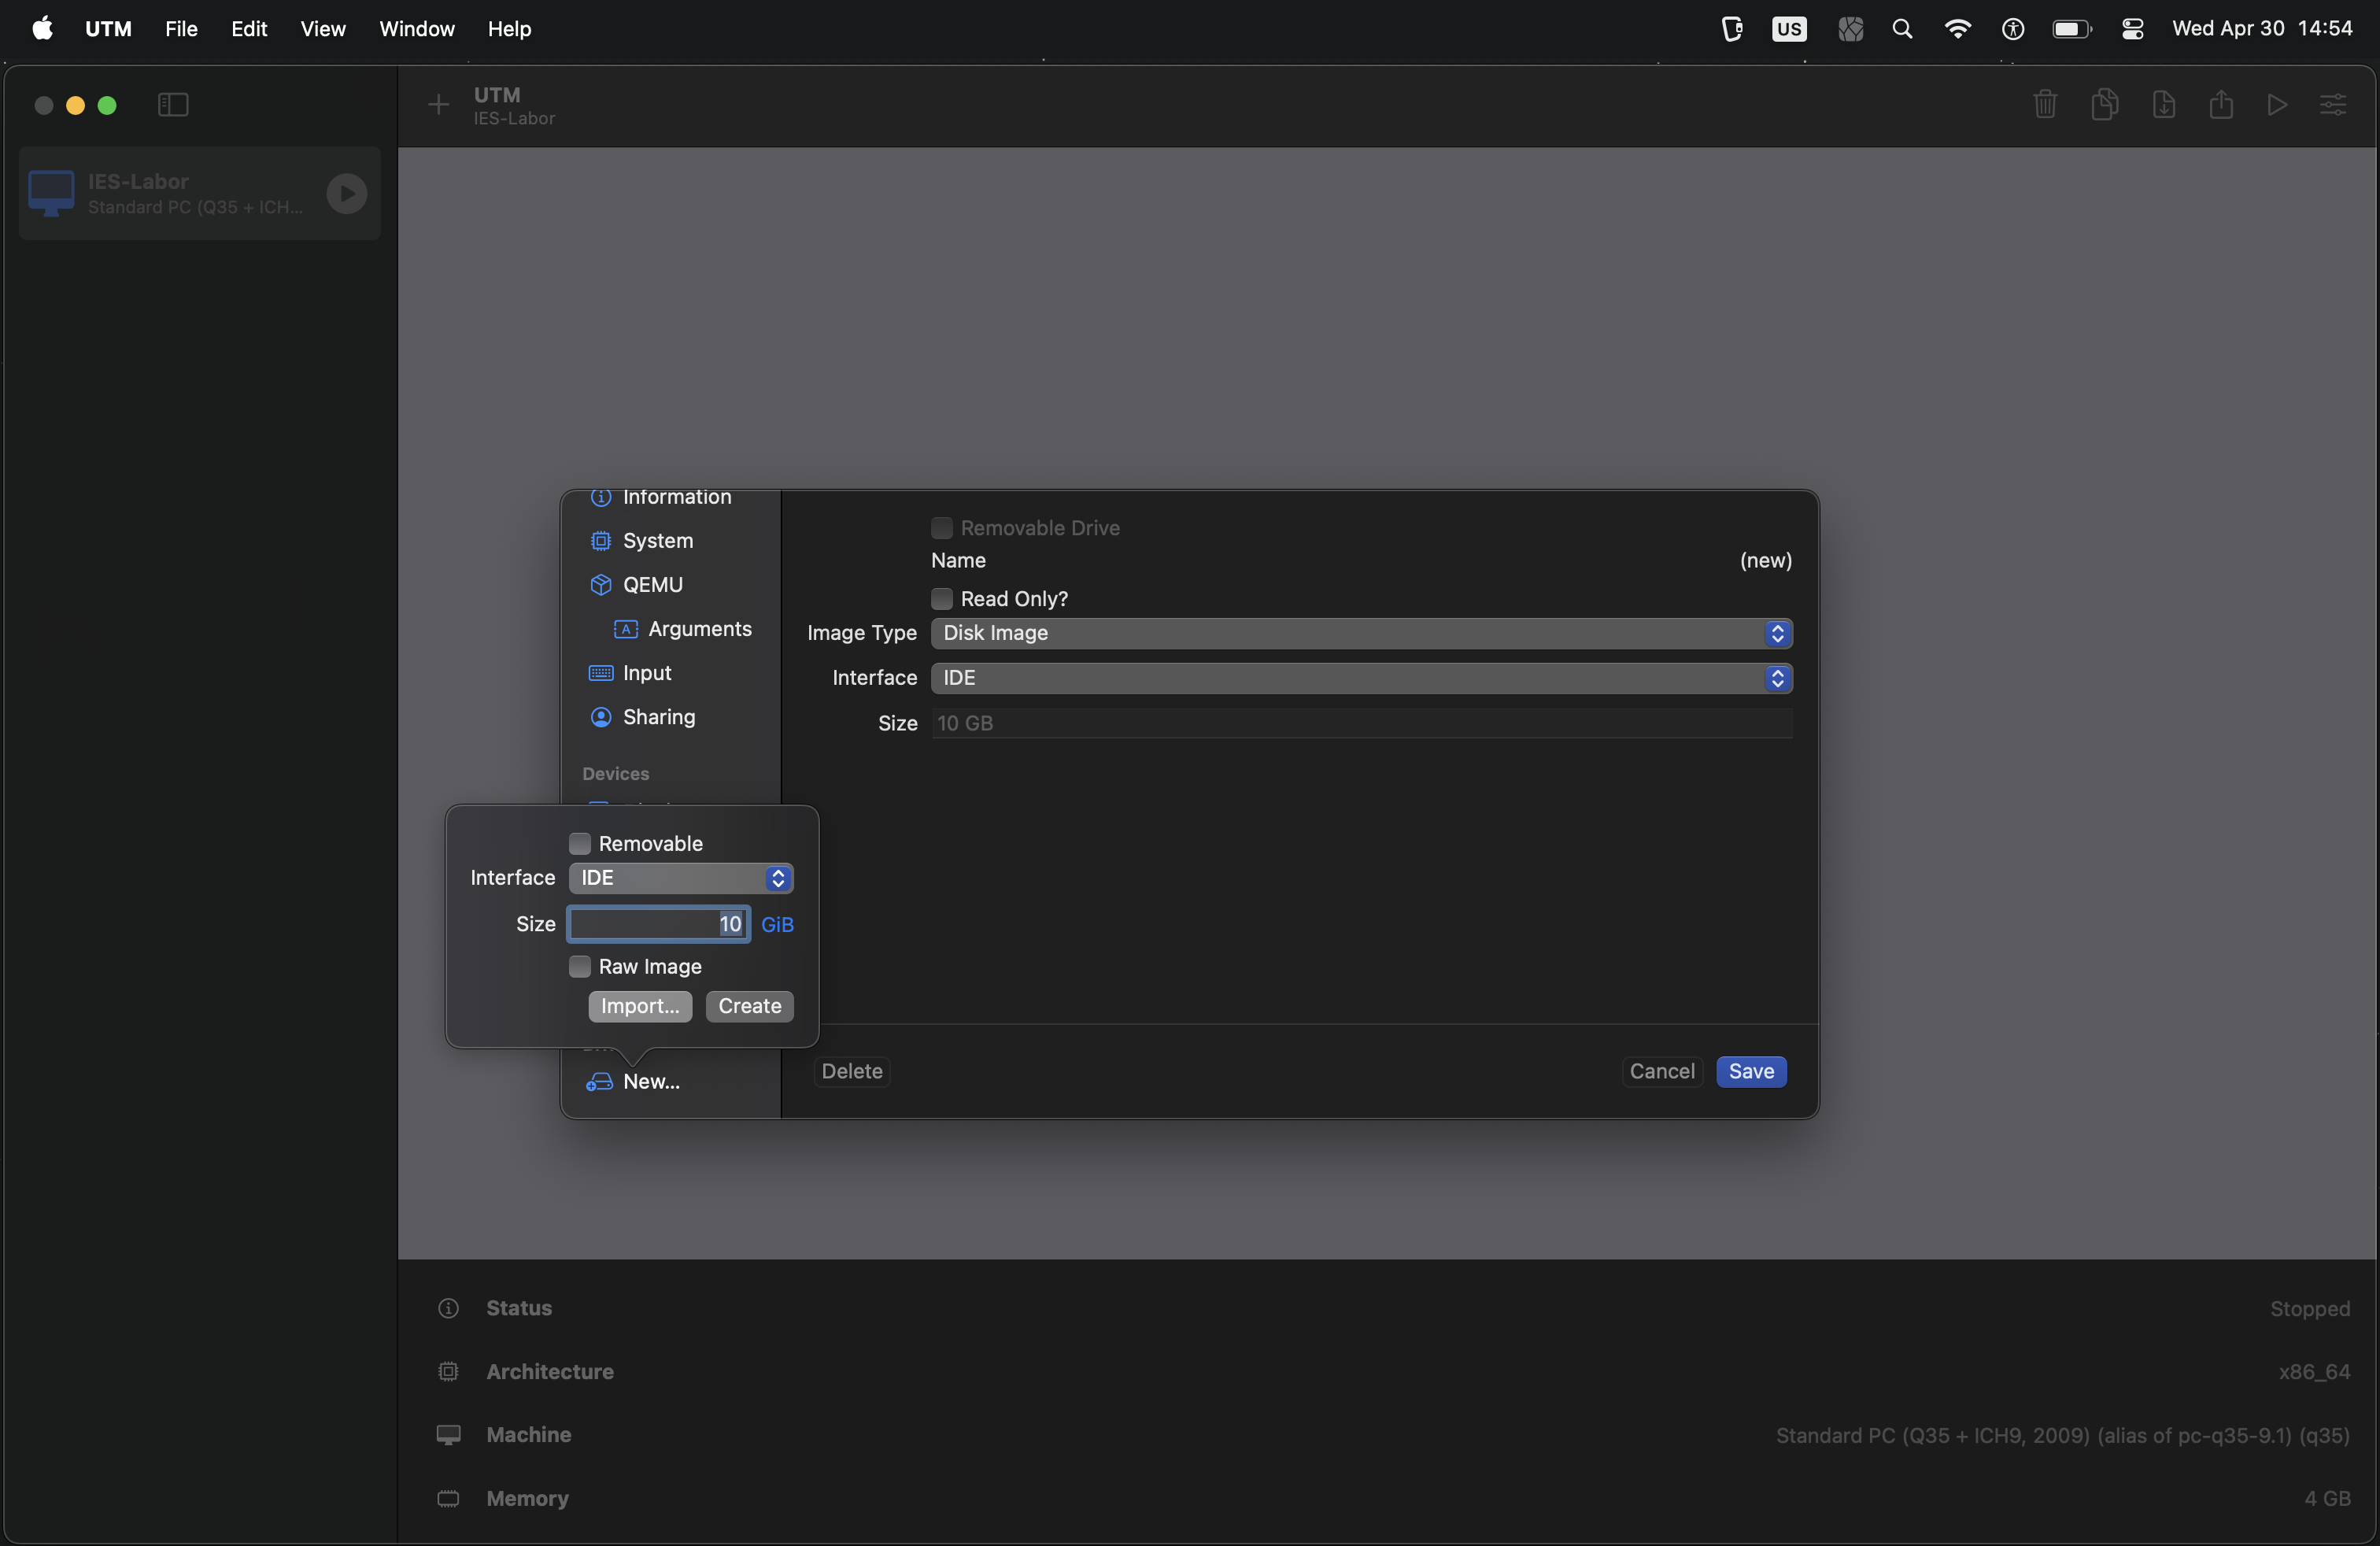
\includegraphics[width=0.48\textwidth]{images/img_utm_disk-import.png}
    \caption{Löschen der vorhandenen Disk und Import einer neuen}
    \label{fig:disk-manage}
\end{figure}

Die Durchführung der Schritte 8-9 ist in Abbildung \ref{fig:disk-manage} zu sehen.

\begin{enumerate}[label=\arabic*.,leftmargin=1.5em,itemsep=0.3em,start=10]
  \item Importieren Sie die neu konvertierte Datei (falls nicht geändert, liegt diese noch im Download-Verzeichnis mit dem Namen \datei{IES-Labor.qcow2})
\end{enumerate}

\begin{figure}[H]
    \centering
    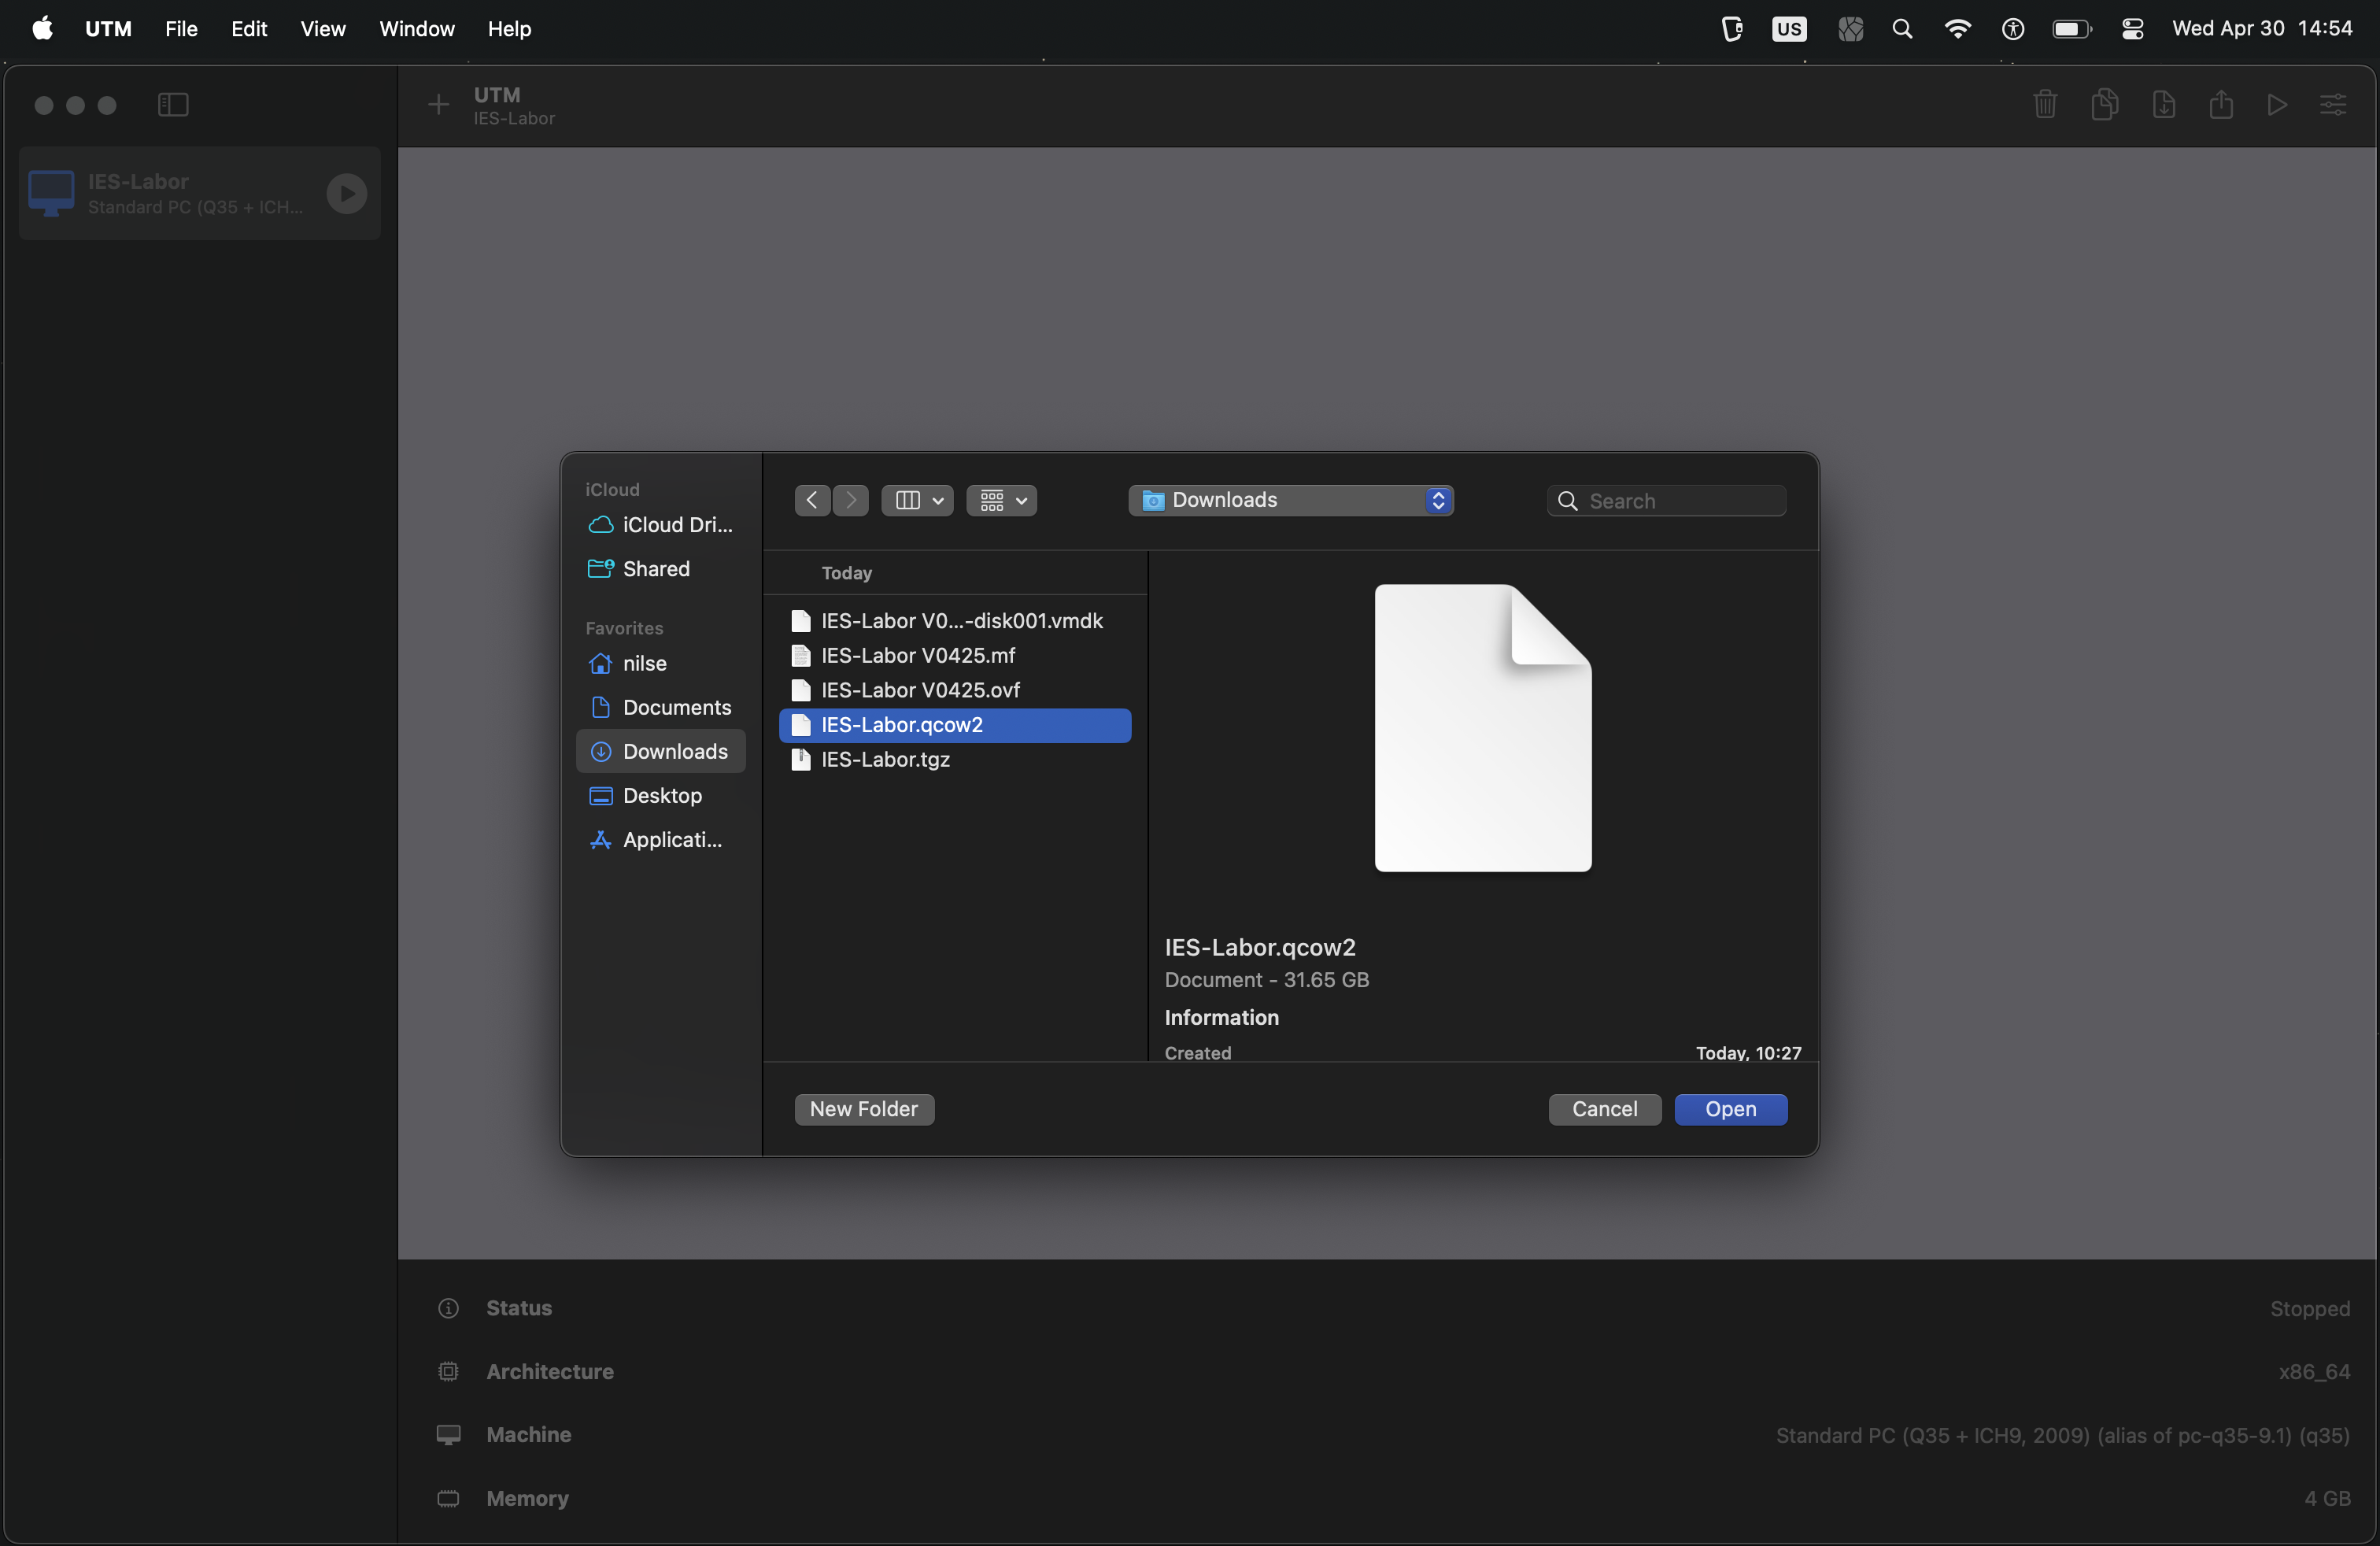
\includegraphics[width=0.7\textwidth]{images/img_utm_disk-import-converted-file.png}
    \caption{Import der konvertierten Disk-Datei}
    \label{fig:disk-import}
\end{figure}

Der Import der konvertierten Datei gemäß Schritt 10 ist in Abbildung \ref{fig:disk-import} dargestellt.

\begin{enumerate}[label=\arabic*.,leftmargin=1.5em,itemsep=0.3em,start=11]
  \item Speichern Sie die Änderungen
  \item Starten Sie die VM
\end{enumerate}

\begin{figure}[H]
    \centering
    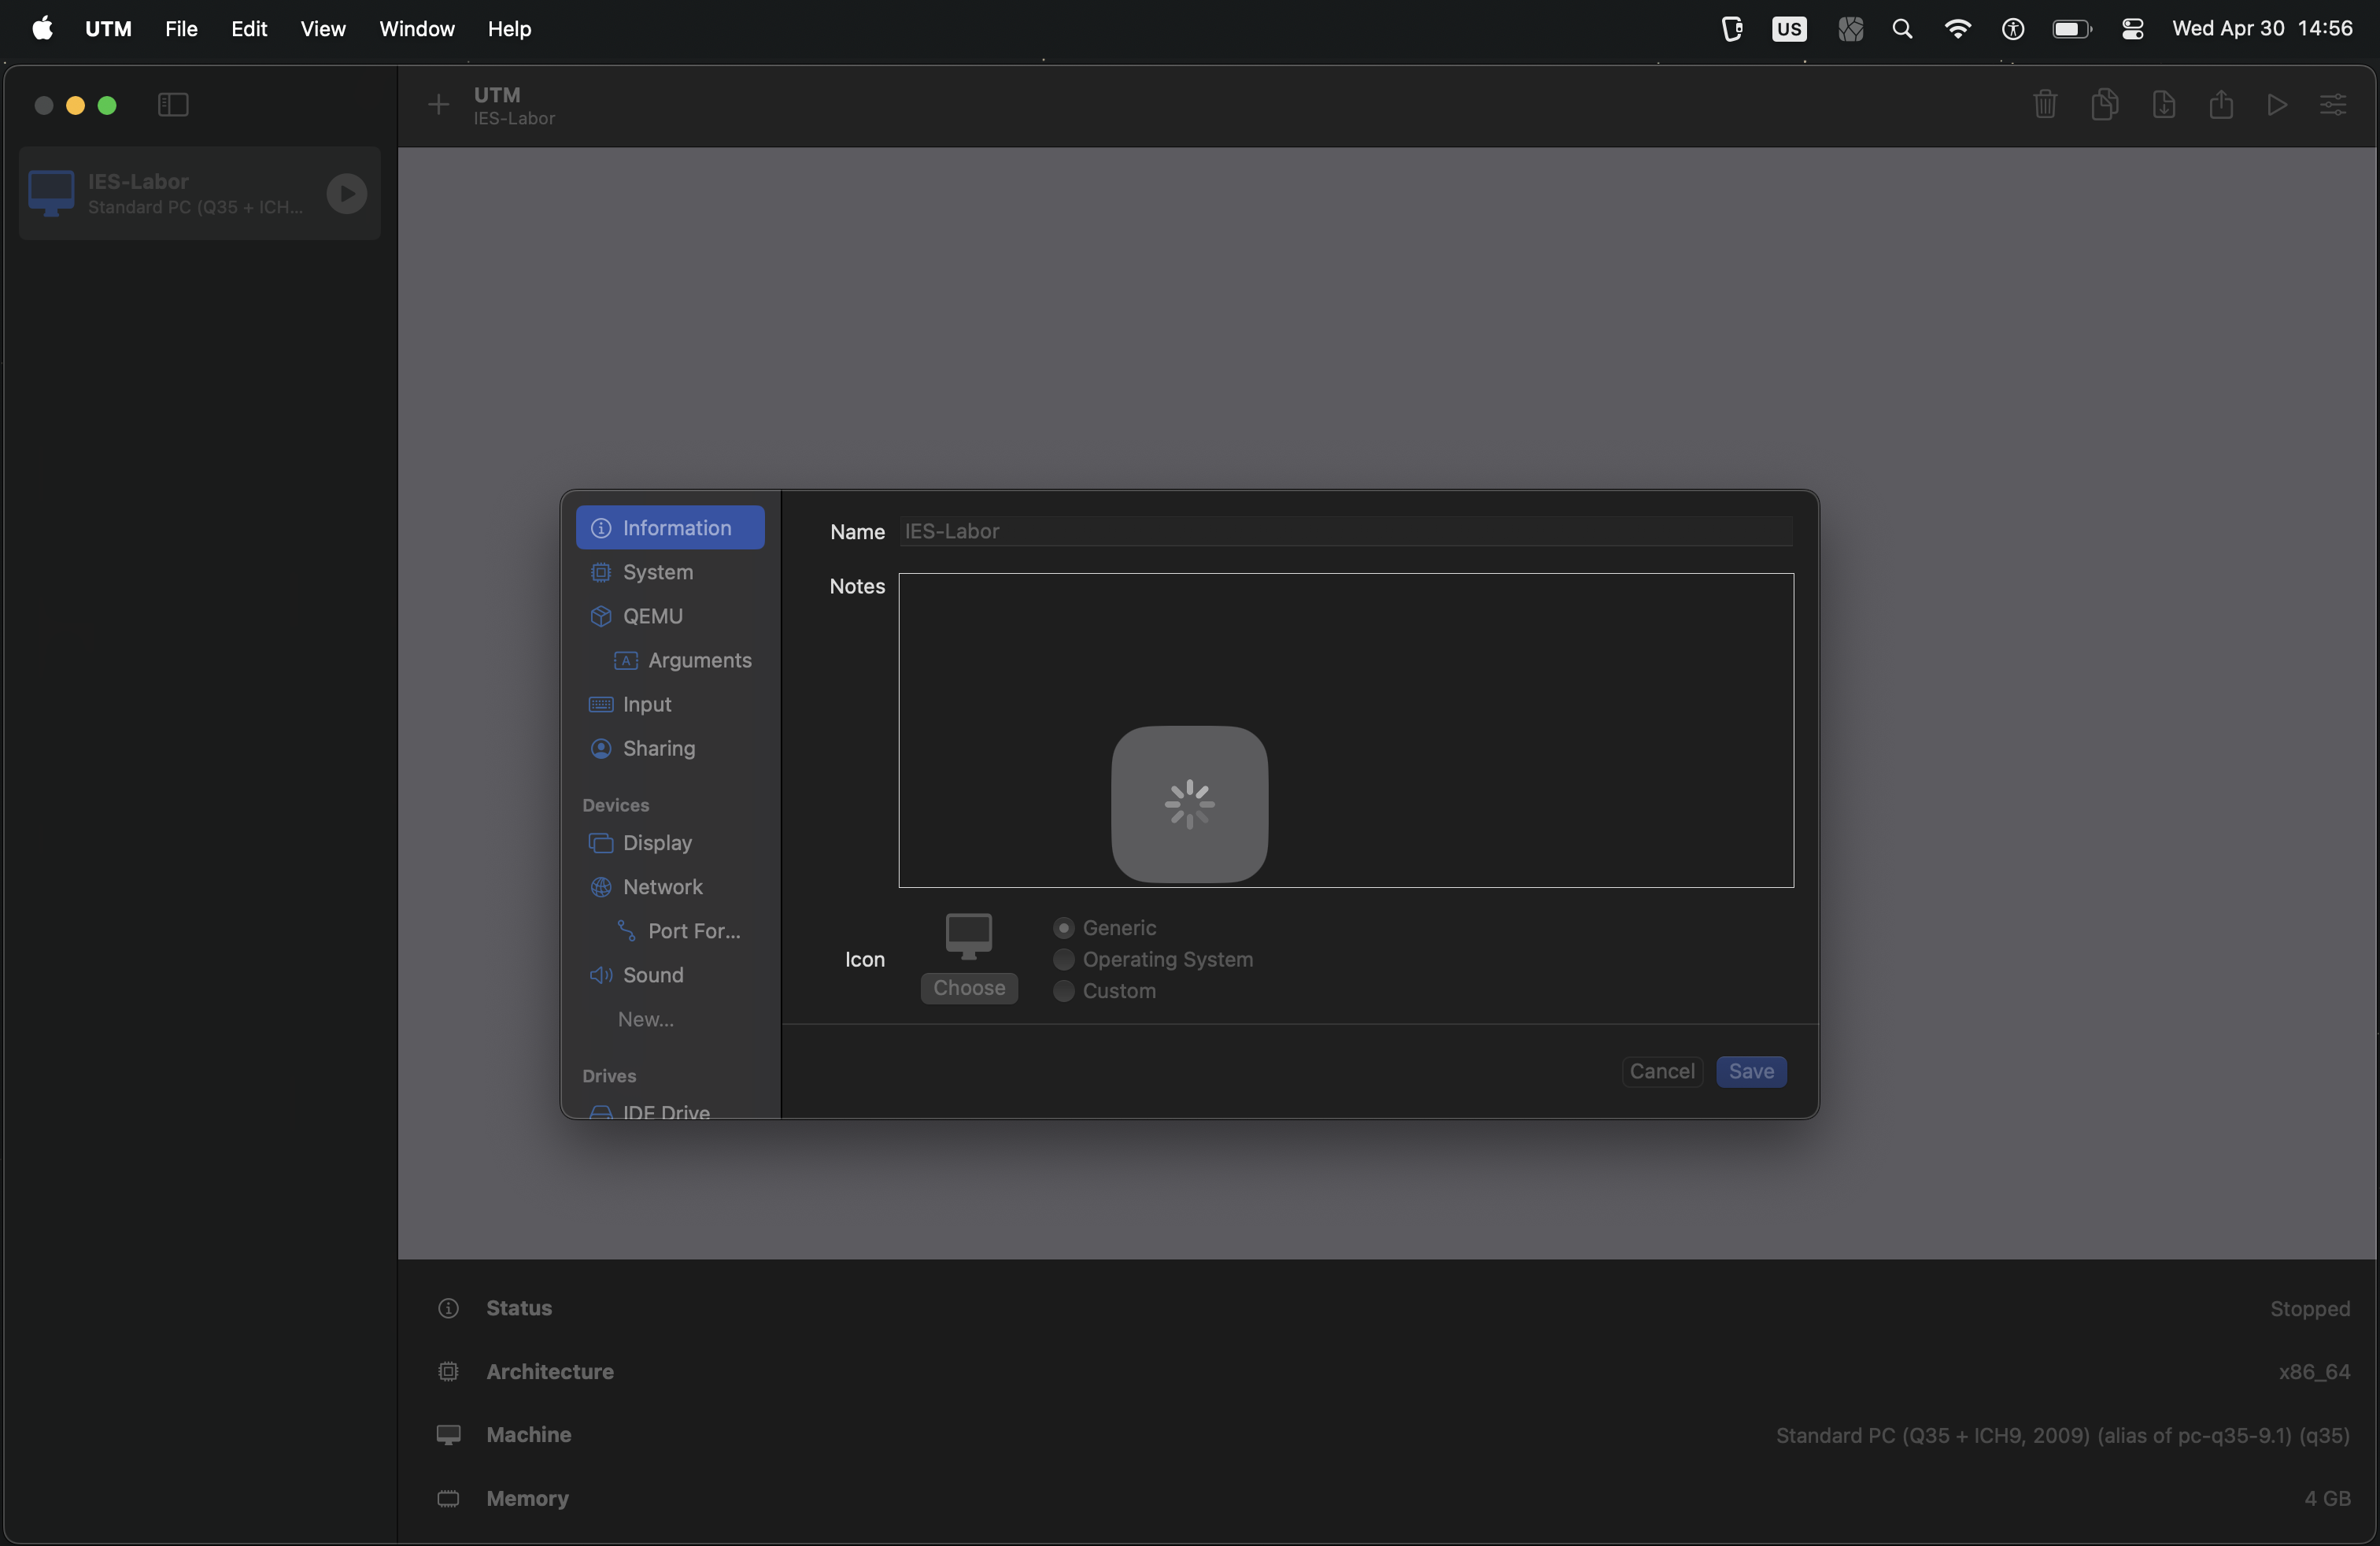
\includegraphics[width=0.48\textwidth]{images/img_utm_save.png}
    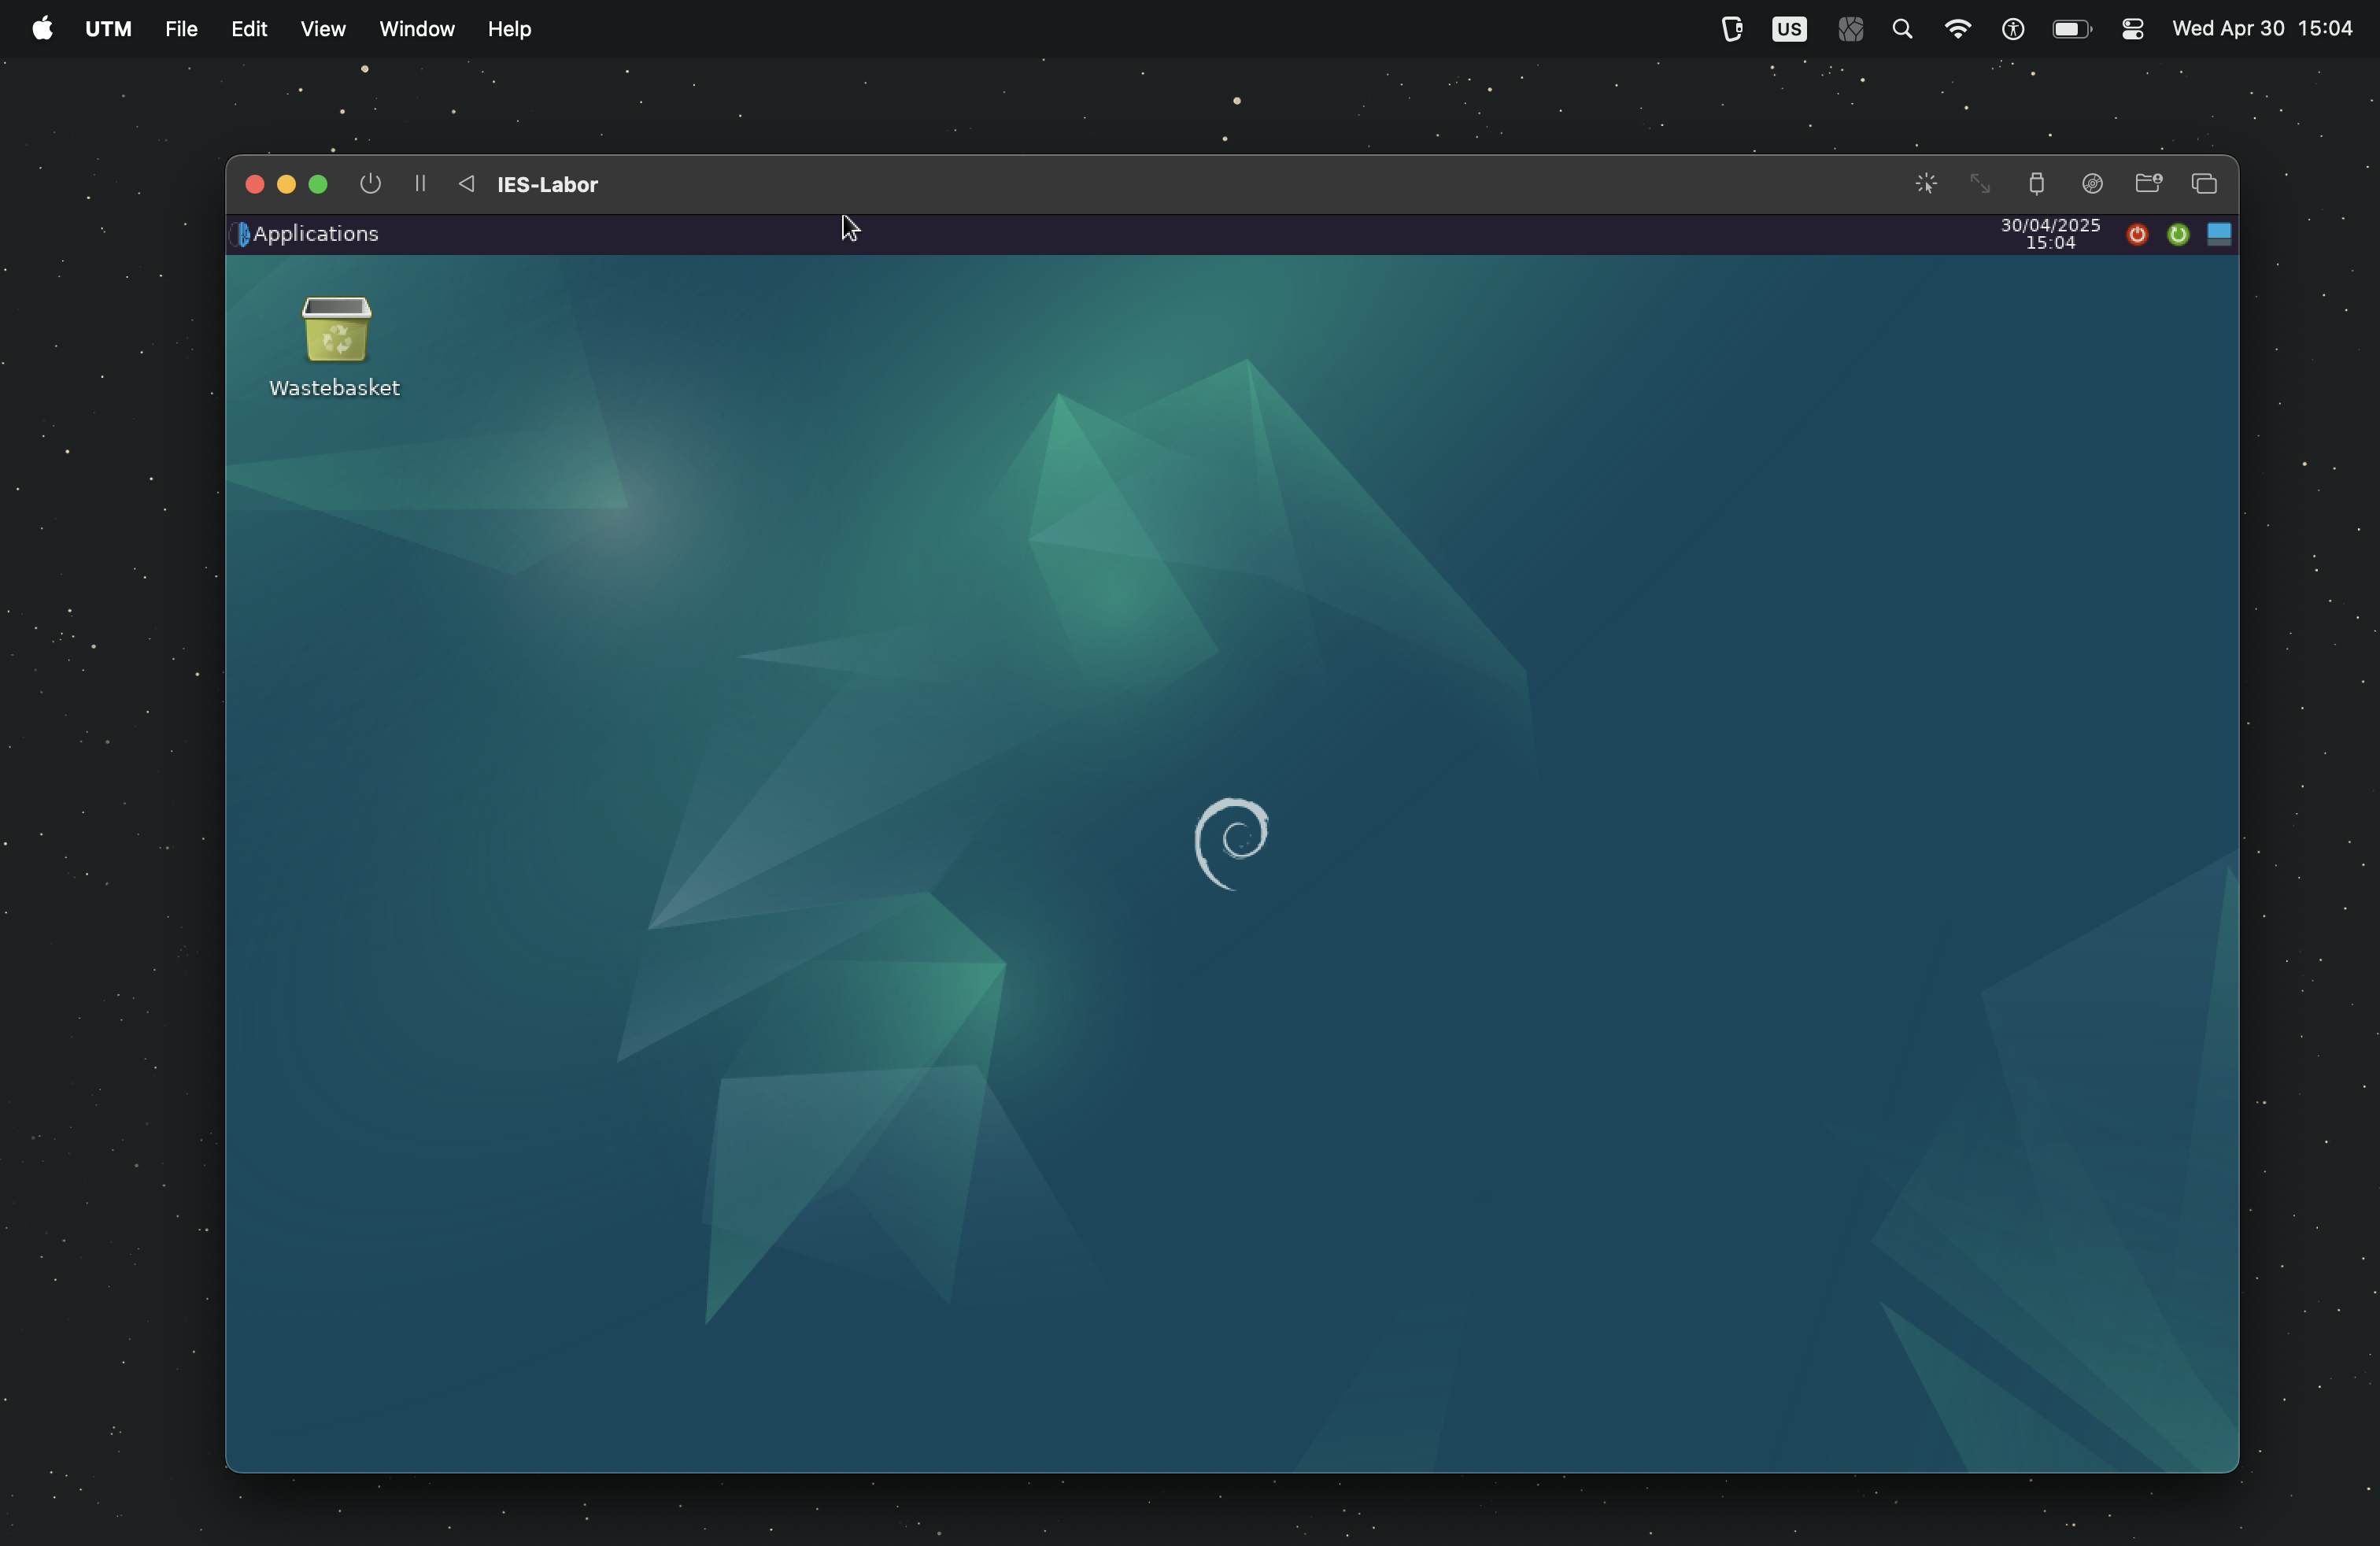
\includegraphics[width=0.48\textwidth]{images/img_utm_labor_running.png}
    \caption{Speichern der Einstellungen und Start der VM}
    \label{fig:save-start}
\end{figure}

Die Durchführung der Schritte 11-12 ist in Abbildung \ref{fig:save-start} zu sehen.

\end{document}
